\documentclass[journal,12pt,twocolumn]{IEEEtran}
%
\usepackage{setspace}
\usepackage{gensymb}
%\doublespacing
\singlespacing

%\usepackage{graphicx}
%\usepackage{amssymb}
%\usepackage{relsize}
\usepackage[cmex10]{amsmath}
%\usepackage{amsthm}
%\interdisplaylinepenalty=2500
%\savesymbol{iint}
%\usepackage{txfonts}
%\restoresymbol{TXF}{iint}
%\usepackage{wasysym}
\usepackage{amsthm}
%\usepackage{iithtlc}
\usepackage{mathrsfs}
\usepackage{txfonts}
\usepackage{stfloats}
\usepackage{bm}
\usepackage{cite}
\usepackage{cases}
\usepackage{subfig}
%\usepackage{xtab}
\usepackage{longtable}
\usepackage{multirow}
%\usepackage{algorithm}
%\usepackage{algpseudocode}
\usepackage{enumitem}
\usepackage{mathtools}
\usepackage{steinmetz}
\usepackage{tikz}
\usepackage{circuitikz}
\usepackage{verbatim}
\usepackage{tfrupee}
\usepackage[breaklinks=true]{hyperref}
%\usepackage{stmaryrd}
\usepackage{tkz-euclide} % loads  TikZ and tkz-base
\usetkzobj{all}
\usetikzlibrary{decorations.markings}
\usetikzlibrary{shapes.geometric}
\newif\iflabrev
\usepackage{listings}
    \usepackage{color}                                            %%
    \usepackage{array}                                            %%
    \usepackage{longtable}                                        %%
    \usepackage{calc}                                             %%
    \usepackage{multirow}                                         %%
    \usepackage{hhline}                                           %%
    \usepackage{ifthen}                                           %%
  %optionally (for landscape tables embedded in another document): %%
    \usepackage{lscape}     
\usepackage{multicol}
\usepackage{chngcntr}
%\usepackage{enumerate}

%\usepackage{wasysym}
%\newcounter{MYtempeqncnt}
\DeclareMathOperator*{\Res}{Res}
%\renewcommand{\baselinestretch}{2}
\renewcommand\thesection{\arabic{section}}
\renewcommand\thesubsection{\thesection.\arabic{subsection}}
\renewcommand\thesubsubsection{\thesubsection.\arabic{subsubsection}}

\renewcommand\thesectiondis{\arabic{section}}
\renewcommand\thesubsectiondis{\thesectiondis.\arabic{subsection}}
\renewcommand\thesubsubsectiondis{\thesubsectiondis.\arabic{subsubsection}}

% correct bad hyphenation here
\hyphenation{op-tical net-works semi-conduc-tor}
\def\inputGnumericTable{}                                 %%

\lstset{
%language=C,
frame=single, 
breaklines=true,
columns=fullflexible
}
%\lstset{
%language=tex,
%frame=single, 
%breaklines=true
%}

\begin{document}
%


\newtheorem{theorem}{Theorem}[section]
\newtheorem{problem}{Problem}
\newtheorem{proposition}{Proposition}[section]
\newtheorem{lemma}{Lemma}[section]
\newtheorem{corollary}[theorem]{Corollary}
\newtheorem{example}{Example}[section]
\newtheorem{definition}[problem]{Definition}
%\newtheorem{thm}{Theorem}[section] 
%\newtheorem{defn}[thm]{Definition}
%\newtheorem{algorithm}{Algorithm}[section]
%\newtheorem{cor}{Corollary}
\newcommand{\BEQA}{\begin{eqnarray}}
\newcommand{\EEQA}{\end{eqnarray}}
\newcommand{\define}{\stackrel{\triangle}{=}}

\bibliographystyle{IEEEtran}
%\bibliographystyle{ieeetr}


\providecommand{\mbf}{\mathbf}
\providecommand{\pr}[1]{\ensuremath{\Pr\left(#1\right)}}
\providecommand{\qfunc}[1]{\ensuremath{Q\left(#1\right)}}
\providecommand{\sbrak}[1]{\ensuremath{{}\left[#1\right]}}
\providecommand{\lsbrak}[1]{\ensuremath{{}\left[#1\right.}}
\providecommand{\rsbrak}[1]{\ensuremath{{}\left.#1\right]}}
\providecommand{\brak}[1]{\ensuremath{\left(#1\right)}}
\providecommand{\lbrak}[1]{\ensuremath{\left(#1\right.}}
\providecommand{\rbrak}[1]{\ensuremath{\left.#1\right)}}
\providecommand{\cbrak}[1]{\ensuremath{\left\{#1\right\}}}
\providecommand{\lcbrak}[1]{\ensuremath{\left\{#1\right.}}
\providecommand{\rcbrak}[1]{\ensuremath{\left.#1\right\}}}
\theoremstyle{remark}
\newtheorem{rem}{Remark}
\newcommand{\sgn}{\mathop{\mathrm{sgn}}}
\providecommand{\abs}[1]{\left\vert#1\right\vert}
\providecommand{\res}[1]{\Res\displaylimits_{#1}} 
\providecommand{\norm}[1]{\left\lVert#1\right\rVert}
%\providecommand{\norm}[1]{\lVert#1\rVert}
\providecommand{\mtx}[1]{\mathbf{#1}}
\providecommand{\mean}[1]{E\left[ #1 \right]}
\providecommand{\fourier}{\overset{\mathcal{F}}{ \rightleftharpoons}}
%\providecommand{\hilbert}{\overset{\mathcal{H}}{ \rightleftharpoons}}
\providecommand{\system}{\overset{\mathcal{H}}{ \longleftrightarrow}}
	%\newcommand{\solution}[2]{\textbf{Solution:}{#1}}
\newcommand{\solution}{\noindent \textbf{Solution: }}
\newcommand{\cosec}{\,\text{cosec}\,}
\providecommand{\dec}[2]{\ensuremath{\overset{#1}{\underset{#2}{\gtrless}}}}
\newcommand{\myvec}[1]{\ensuremath{\begin{pmatrix}#1\end{pmatrix}}}
\newcommand{\mydet}[1]{\ensuremath{\begin{vmatrix}#1\end{vmatrix}}}
%\numberwithin{equation}{section}
\numberwithin{equation}{subsection}
\numberwithin{figure}{subsection}
\numberwithin{table}{subsection}
%\numberwithin{problem}{section}
%\numberwithin{definition}{section}
\makeatletter
%\@addtoreset{figure}{problem}
\makeatother

%\let\StandardTheFigure\thefigure
\let\vec\mathbf
%\renewcommand{\thefigure}{\theproblem.\arabic{figure}}
%\renewcommand{\thefigure}{\theproblem}
%\setlist[enumerate,1]{before=\renewcommand\theequation{\theenumi.\arabic{equation}}
%\counterwithin{equation}{enumi}


%\renewcommand{\theequation}{\arabic{subsection}.\arabic{equation}}

\def\putbox#1#2#3{\makebox[0in][l]{\makebox[#1][l]{}\raisebox{\baselineskip}[0in][0in]{\raisebox{#2}[0in][0in]{#3}}}}
     \def\rightbox#1{\makebox[0in][r]{#1}}
     \def\centbox#1{\makebox[0in]{#1}}
     \def\topbox#1{\raisebox{-\baselineskip}[0in][0in]{#1}}
     \def\midbox#1{\raisebox{-0.5\baselineskip}[0in][0in]{#1}}

\vspace{3cm}

\title{
%	\logo{
Control Systems
%	}
}
\author{ G V V Sharma$^{*}$% <-this % stops a space
	\thanks{*The author is with the Department
		of Electrical Engineering, Indian Institute of Technology, Hyderabad
		502285 India e-mail:  gadepall@iith.ac.in. All content in this manual is released under GNU GPL.  Free and open source.}
	
}	
%\title{
%	\logo{Matrix Analysis through Octave}{\begin{center}\includegraphics[scale=.24]{tlc}\end{center}}{}{HAMDSP}
%}


% paper title
% can use linebreaks \\ within to get better formatting as desired
%\title{Matrix Analysis through Octave}
%
%
% author names and IEEE memberships
% note positions of commas and nonbreaking spaces ( ~ ) LaTeX will not break
% a structure at a ~ so this keeps an author's name from being broken across
% two lines.
% use \thanks{} to gain access to the first footnote area
% a separate \thanks must be used for each paragraph as LaTeX2e's \thanks
% was not built to handle multiple paragraphs
%

%\author{<-this % stops a space
%\thanks{}}
%}
% note the % following the last \IEEEmembership and also \thanks - 
% these prevent an unwanted space from occurring between the last author name
% and the end of the author line. i.e., if you had this:
% 
% \author{....lastname \thanks{...} \thanks{...} }
%                     ^------------^------------^----Do not want these spaces!
%
% a space would be appended to the last name and could cause every name on that
% line to be shifted left slightly. This is one of those "LaTeX things". For
% instance, "\textbf{A} \textbf{B}" will typeset as "A B" not "AB". To get
% "AB" then you have to do: "\textbf{A}\textbf{B}"
% \thanks is no different in this regard, so shield the last } of each \thanks
% that ends a line with a % and do not let a space in before the next \thanks.
% Spaces after \IEEEmembership other than the last one are OK (and needed) as
% you are supposed to have spaces between the names. For what it is worth,
% this is a minor point as most people would not even notice if the said evil
% space somehow managed to creep in.



% The paper headers
%\markboth{Journal of \LaTeX\ Class Files,~Vol.~6, No.~1, January~2007}%
%{Shell \MakeLowercase{\textit{et al.}}: Bare Demo of IEEEtran.cls for Journals}
% The only time the second header will appear is for the odd numbered pages
% after the title page when using the twoside option.
% 
% *** Note that you probably will NOT want to include the author's ***
% *** name in the headers of peer review papers.                   ***
% You can use \ifCLASSOPTIONpeerreview for conditional compilation here if
% you desire.




% If you want to put a publisher's ID mark on the page you can do it like
% this:
%\IEEEpubid{0000--0000/00\$00.00~\copyright~2007 IEEE}
% Remember, if you use this you must call \IEEEpubidadjcol in the second
% column for its text to clear the IEEEpubid mark.



% make the title area
\maketitle

\newpage

\tableofcontents

\bigskip

%\renewcommand{\thefigure}{\theenumi}
%\renewcommand{\thefigure}{\thesubsection}
%\renewcommand{\thetable}{\theenumi}
%\renewcommand{\thefigure}{\theproblem}

%\renewcommand{\theequation}{\theenumi}

%\begin{abstract}
%%\boldmath
%In this letter, an algorithm for evaluating the exact analytical bit error rate  (BER)  for the piecewise linear (PL) combiner for  multiple relays is presented. Previous results were available only for upto three relays. The algorithm is unique in the sense that  the actual mathematical expressions, that are prohibitively large, need not be explicitly obtained. The diversity gain due to multiple relays is shown through plots of the analytical BER, well supported by simulations. 
%
%\end{abstract}
% IEEEtran.cls defaults to using nonbold math in the Abstract.
% This preserves the distinction between vectors and scalars. However,
% if the journal you are submitting to favors bold math in the abstract,
% then you can use LaTeX's standard command \boldmath at the very start
% of the abstract to achieve this. Many IEEE journals frown on math
% in the abstract anyway.

% Note that keywords are not normally used for peerreview papers.
%\begin{IEEEkeywords}
%Cooperative diversity, decode and forward, piecewise linear
%\end{IEEEkeywords}



% For peer review papers, you can put extra information on the cover
% page as needed:
% \ifCLASSOPTIONpeerreview
% \begin{center} \bfseries EDICS Category: 3-BBND \end{center}
% \fi
%
% For peerreview papers, this IEEEtran command inserts a page break and
% creates the second title. It will be ignored for other modes.
%\IEEEpeerreviewmaketitle

\begin{abstract}
The objective of this manual is to introduce control system design at an elementary level.
\end{abstract}
Download python codes using 
\begin{lstlisting}
svn co https://github.com/gadepall/school/trunk/control/ketan/codes
\end{lstlisting}


\section{Frequency Response Analysis}
\subsection{Polar Plot}
\begin{enumerate}[label=\thesubsection.\arabic*.,ref=\thesubsection.\theenumi]
\begin{enumerate}[label=\thesubsection.\arabic*.,ref=\thesubsection.\theenumi]
\numberwithin{equation}{enumi}
\item List the different kinds of damping for a second order system defined by 
\begin{align}
\label{eq:ee18btech11012_second}
H(s)=\frac{\omega^2}{s^2+2\zeta\omega+\omega^2}
\end{align}
where $\omega$ is  the natural   frequency  and $ \zeta $  is the  damping factor.
%
\\
\solution The details are available in Table \ref{table:ee18btech11012}
\begin{table}[!ht]
\centering
\begin{enumerate}[label=\thesubsection.\arabic*.,ref=\thesubsection.\theenumi]
\numberwithin{equation}{enumi}
\item List the different kinds of damping for a second order system defined by 
\begin{align}
\label{eq:ee18btech11012_second}
H(s)=\frac{\omega^2}{s^2+2\zeta\omega+\omega^2}
\end{align}
where $\omega$ is  the natural   frequency  and $ \zeta $  is the  damping factor.
%
\\
\solution The details are available in Table \ref{table:ee18btech11012}
\begin{table}[!ht]
\centering
\begin{enumerate}[label=\thesubsection.\arabic*.,ref=\thesubsection.\theenumi]
\numberwithin{equation}{enumi}
\item List the different kinds of damping for a second order system defined by 
\begin{align}
\label{eq:ee18btech11012_second}
H(s)=\frac{\omega^2}{s^2+2\zeta\omega+\omega^2}
\end{align}
where $\omega$ is  the natural   frequency  and $ \zeta $  is the  damping factor.
%
\\
\solution The details are available in Table \ref{table:ee18btech11012}
\begin{table}[!ht]
\centering
\input{./tables/ee18btech11012.tex}
\caption{}
\label{table:ee18btech11012}
\end{table}

\item Classify the following second-order systems according to damping.
\label{prob:ee18btech11012_damp}
\begin{enumerate}
\item $H(s) = \frac{15}{{s^2+5s+15}}$ 
\item $H(s) = \frac{25}{{s^2+10s+25}}$
\item $H(s) =\frac{35}{{s^2+18s+35}}$ 
\end{enumerate}
\solution For 
\begin{align}
H(s) &= \frac{25}{{s^2+10s+25}},
\\
     \omega^2 &= 25,   2\zeta\omega =10\\
\implies  \omega &=1,  {\zeta} = 1
\end{align}
and the system is critically damped.  Similarly, the damping factors for other systems in Problem \ref{prob:ee18btech11012_damp} are calculated and listed in Table \ref{table:ee18btech11012_damp}
%
\begin{table}[!ht]
\centering
\input{./tables/ee18btech11012_damp.tex}
\caption{}
\label{table:ee18btech11012_damp}
\end{table}

\item Find the step response of each $H(s)$ in Table \ref{table:ee18btech11012_damp}.
\\
\solution 
\begin{enumerate}
\item For 
\begin{align}
 H(s)=\frac{15}{s^2+5s+15},
\end{align}
%
the step response is
\begin{equation}
y(t)=25te^{-5t}u(t)
\label{eq:ee18btech11012_over}
\end{equation}
\item For 
%
\begin{align}
H(s)=\frac{25}{s^2+10s+25},
\end{align}
%
the step response is
\begin{equation}
y(t)=\frac{30}{\sqrt{35}}e^{\frac{-5t}{2}}\sin\brak{\frac{\sqrt{35}}{2}t}u(t)
\label{eq:ee18btech11012_critical}
\end{equation}
\item  For 

\begin{align}
H(s)=\frac{35}{s^2+18s+35},
\end{align}
the step response is
\begin{equation}
    y(t)=\frac{35}{2\sqrt{46}}\sbrak{e^{(-9+\sqrt{46})t}-e^{(-9-\sqrt{46})t}}u(t)
\label{eq:ee18btech11012_under}
\end{equation}
\end{enumerate}
\item Illustrate the effect of damping by plotting the step responses in \eqref{eq:ee18btech11012_over}-\eqref{eq:ee18btech11012_under}
\\
\solution The following code
\begin{lstlisting}
codes/ee18btech11012.py
\end{lstlisting}
%
plots the desired graphs in
Fig.     \ref{fig:ee18btech11012}. 
%
%\begin{figure}[ht!]
%    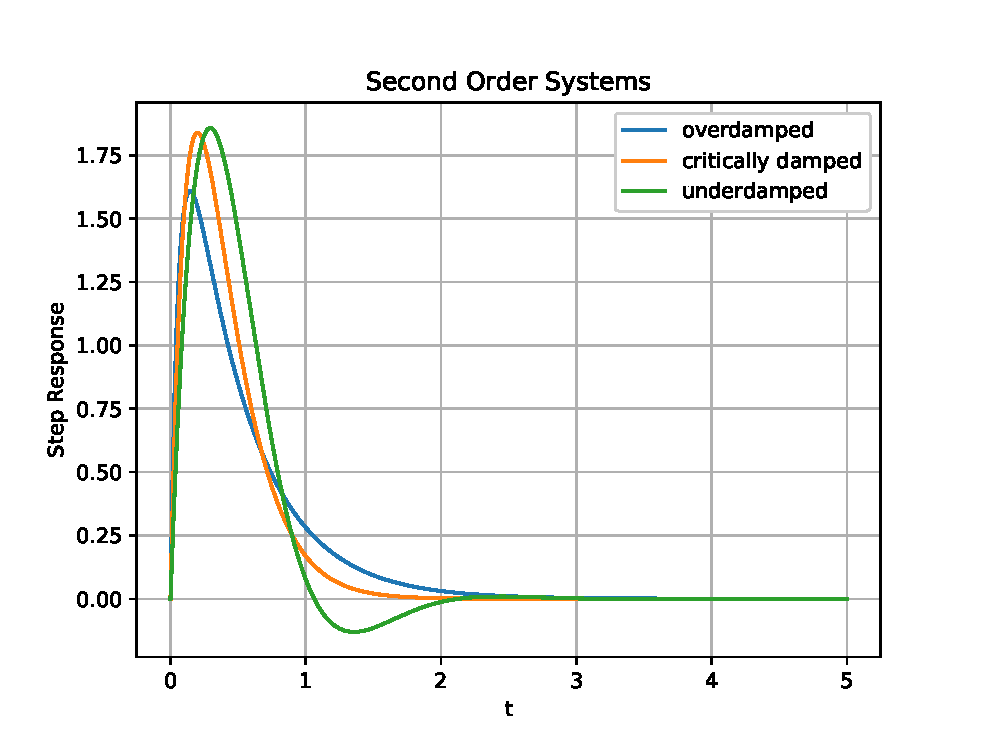
\includegraphics[width=\columnwidth]{./figs/ee18btech11012.eps}
%    \caption{}
%    \label{fig:ee18btech11012}
%\end{figure}

using a Python code to sketch the response.  
\end{enumerate}

\caption{}
\label{table:ee18btech11012}
\end{table}

\item Classify the following second-order systems according to damping.
\label{prob:ee18btech11012_damp}
\begin{enumerate}
\item $H(s) = \frac{15}{{s^2+5s+15}}$ 
\item $H(s) = \frac{25}{{s^2+10s+25}}$
\item $H(s) =\frac{35}{{s^2+18s+35}}$ 
\end{enumerate}
\solution For 
\begin{align}
H(s) &= \frac{25}{{s^2+10s+25}},
\\
     \omega^2 &= 25,   2\zeta\omega =10\\
\implies  \omega &=1,  {\zeta} = 1
\end{align}
and the system is critically damped.  Similarly, the damping factors for other systems in Problem \ref{prob:ee18btech11012_damp} are calculated and listed in Table \ref{table:ee18btech11012_damp}
%
\begin{table}[!ht]
\centering
%%%%%%%%%%%%%%%%%%%%%%%%%%%%%%%%%%%%%%%%%%%%%%%%%%%%%%%%%%%%%%%%%%%%%%
%%                                                                  %%
%%  This is the header of a LaTeX2e file exported from Gnumeric.    %%
%%                                                                  %%
%%  This file can be compiled as it stands or included in another   %%
%%  LaTeX document. The table is based on the longtable package so  %%
%%  the longtable options (headers, footers...) can be set in the   %%
%%  preamble section below (see PRAMBLE).                           %%
%%                                                                  %%
%%  To include the file in another, the following two lines must be %%
%%  in the including file:                                          %%
%%        \def\inputGnumericTable{}                                 %%
%%  at the beginning of the file and:                               %%
%%        \input{name-of-this-file.tex}                             %%
%%  where the table is to be placed. Note also that the including   %%
%%  file must use the following packages for the table to be        %%
%%  rendered correctly:                                             %%
%%    \usepackage[latin1]{inputenc}                                 %%
%%    \usepackage{color}                                            %%
%%    \usepackage{array}                                            %%
%%    \usepackage{longtable}                                        %%
%%    \usepackage{calc}                                             %%
%%    \usepackage{multirow}                                         %%
%%    \usepackage{hhline}                                           %%
%%    \usepackage{ifthen}                                           %%
%%  optionally (for landscape tables embedded in another document): %%
%%    \usepackage{lscape}                                           %%
%%                                                                  %%
%%%%%%%%%%%%%%%%%%%%%%%%%%%%%%%%%%%%%%%%%%%%%%%%%%%%%%%%%%%%%%%%%%%%%%



%%  This section checks if we are begin input into another file or  %%
%%  the file will be compiled alone. First use a macro taken from   %%
%%  the TeXbook ex 7.7 (suggestion of Han-Wen Nienhuys).            %%
\def\ifundefined#1{\expandafter\ifx\csname#1\endcsname\relax}


%%  Check for the \def token for inputed files. If it is not        %%
%%  defined, the file will be processed as a standalone and the     %%
%%  preamble will be used.                                          %%
\ifundefined{inputGnumericTable}

%%  We must be able to close or not the document at the end.        %%
	\def\gnumericTableEnd{\end{document}}


%%%%%%%%%%%%%%%%%%%%%%%%%%%%%%%%%%%%%%%%%%%%%%%%%%%%%%%%%%%%%%%%%%%%%%
%%                                                                  %%
%%  This is the PREAMBLE. Change these values to get the right      %%
%%  paper size and other niceties.                                  %%
%%                                                                  %%
%%%%%%%%%%%%%%%%%%%%%%%%%%%%%%%%%%%%%%%%%%%%%%%%%%%%%%%%%%%%%%%%%%%%%%

	\documentclass[12pt%
			  %,landscape%
                    ]{report}
       \usepackage[latin1]{inputenc}
       \usepackage{fullpage}
       \usepackage{color}
       \usepackage{array}
       \usepackage{longtable}
       \usepackage{calc}
       \usepackage{multirow}
       \usepackage{hhline}
       \usepackage{ifthen}

	\begin{document}


%%  End of the preamble for the standalone. The next section is for %%
%%  documents which are included into other LaTeX2e files.          %%
\else

%%  We are not a stand alone document. For a regular table, we will %%
%%  have no preamble and only define the closing to mean nothing.   %%
    \def\gnumericTableEnd{}

%%  If we want landscape mode in an embedded document, comment out  %%
%%  the line above and uncomment the two below. The table will      %%
%%  begin on a new page and run in landscape mode.                  %%
%       \def\gnumericTableEnd{\end{landscape}}
%       \begin{landscape}


%%  End of the else clause for this file being \input.              %%
\fi

%%%%%%%%%%%%%%%%%%%%%%%%%%%%%%%%%%%%%%%%%%%%%%%%%%%%%%%%%%%%%%%%%%%%%%
%%                                                                  %%
%%  The rest is the gnumeric table, except for the closing          %%
%%  statement. Changes below will alter the table's appearance.     %%
%%                                                                  %%
%%%%%%%%%%%%%%%%%%%%%%%%%%%%%%%%%%%%%%%%%%%%%%%%%%%%%%%%%%%%%%%%%%%%%%

\providecommand{\gnumericmathit}[1]{#1} 
%%  Uncomment the next line if you would like your numbers to be in %%
%%  italics if they are italizised in the gnumeric table.           %%
%\renewcommand{\gnumericmathit}[1]{\mathit{#1}}
\providecommand{\gnumericPB}[1]%
{\let\gnumericTemp=\\#1\let\\=\gnumericTemp\hspace{0pt}}
 \ifundefined{gnumericTableWidthDefined}
        \newlength{\gnumericTableWidth}
        \newlength{\gnumericTableWidthComplete}
        \newlength{\gnumericMultiRowLength}
        \global\def\gnumericTableWidthDefined{}
 \fi
%% The following setting protects this code from babel shorthands.  %%
 \ifthenelse{\isundefined{\languageshorthands}}{}{\languageshorthands{english}}
%%  The default table format retains the relative column widths of  %%
%%  gnumeric. They can easily be changed to c, r or l. In that case %%
%%  you may want to comment out the next line and uncomment the one %%
%%  thereafter                                                      %%
\providecommand\gnumbox{\makebox[0pt]}
%%\providecommand\gnumbox[1][]{\makebox}

%% to adjust positions in multirow situations                       %%
\setlength{\bigstrutjot}{\jot}
\setlength{\extrarowheight}{\doublerulesep}

%%  The \setlongtables command keeps column widths the same across  %%
%%  pages. Simply comment out next line for varying column widths.  %%
\setlongtables

\setlength\gnumericTableWidth{%
	36pt+%
	20pt+%
	35pt+%
	91pt+%
0pt}
\def\gumericNumCols{4}
\setlength\gnumericTableWidthComplete{\gnumericTableWidth+%
         \tabcolsep*\gumericNumCols*2+\arrayrulewidth*\gumericNumCols}
\ifthenelse{\lengthtest{\gnumericTableWidthComplete > \linewidth}}%
         {\def\gnumericScale{\ratio{\linewidth-%
                        \tabcolsep*\gumericNumCols*2-%
                        \arrayrulewidth*\gumericNumCols}%
{\gnumericTableWidth}}}%
{\def\gnumericScale{1}}

%%%%%%%%%%%%%%%%%%%%%%%%%%%%%%%%%%%%%%%%%%%%%%%%%%%%%%%%%%%%%%%%%%%%%%
%%                                                                  %%
%% The following are the widths of the various columns. We are      %%
%% defining them here because then they are easier to change.       %%
%% Depending on the cell formats we may use them more than once.    %%
%%                                                                  %%
%%%%%%%%%%%%%%%%%%%%%%%%%%%%%%%%%%%%%%%%%%%%%%%%%%%%%%%%%%%%%%%%%%%%%%

\ifthenelse{\isundefined{\gnumericColA}}{\newlength{\gnumericColA}}{}\settowidth{\gnumericColA}{\begin{tabular}{@{}p{36pt*\gnumericScale}@{}}x\end{tabular}}
\ifthenelse{\isundefined{\gnumericColB}}{\newlength{\gnumericColB}}{}\settowidth{\gnumericColB}{\begin{tabular}{@{}p{20pt*\gnumericScale}@{}}x\end{tabular}}
\ifthenelse{\isundefined{\gnumericColC}}{\newlength{\gnumericColC}}{}\settowidth{\gnumericColC}{\begin{tabular}{@{}p{35pt*\gnumericScale}@{}}x\end{tabular}}
\ifthenelse{\isundefined{\gnumericColD}}{\newlength{\gnumericColD}}{}\settowidth{\gnumericColD}{\begin{tabular}{@{}p{91pt*\gnumericScale}@{}}x\end{tabular}}

\begin{tabular}[c]{%
	b{\gnumericColA}%
	b{\gnumericColB}%
	b{\gnumericColC}%
	b{\gnumericColD}%
	}

%%%%%%%%%%%%%%%%%%%%%%%%%%%%%%%%%%%%%%%%%%%%%%%%%%%%%%%%%%%%%%%%%%%%%%
%%  The longtable options. (Caption, headers... see Goosens, p.124) %%
%	\caption{The Table Caption.}             \\	%
% \hline	% Across the top of the table.
%%  The rest of these options are table rows which are placed on    %%
%%  the first, last or every page. Use \multicolumn if you want.    %%

%%  Header for the first page.                                      %%
%	\multicolumn{4}{c}{The First Header} \\ \hline 
%	\multicolumn{1}{c}{colTag}	%Column 1
%	&\multicolumn{1}{c}{colTag}	%Column 2
%	&\multicolumn{1}{c}{colTag}	%Column 3
%	&\multicolumn{1}{c}{colTag}	\\ \hline %Last column
%	\endfirsthead

%%  The running header definition.                                  %%
%	\hline
%	\multicolumn{4}{l}{\ldots\small\slshape continued} \\ \hline
%	\multicolumn{1}{c}{colTag}	%Column 1
%	&\multicolumn{1}{c}{colTag}	%Column 2
%	&\multicolumn{1}{c}{colTag}	%Column 3
%	&\multicolumn{1}{c}{colTag}	\\ \hline %Last column
%	\endhead

%%  The running footer definition.                                  %%
%	\hline
%	\multicolumn{4}{r}{\small\slshape continued\ldots} \\
%	\endfoot

%%  The ending footer definition.                                   %%
%	\multicolumn{4}{c}{That's all folks} \\ \hline 
%	\endlastfoot
%%%%%%%%%%%%%%%%%%%%%%%%%%%%%%%%%%%%%%%%%%%%%%%%%%%%%%%%%%%%%%%%%%%%%%

\hhline{|-|-|-|-}
	 \multicolumn{1}{|p{\gnumericColA}|}%
	{\gnumericPB{\centering}\gnumbox{\textbf{H(s)}}}
	&\multicolumn{1}{p{\gnumericColB}|}%
	{\gnumericPB{\centering}\gnumbox{\textbf{$\omega$}}}
	&\multicolumn{1}{p{\gnumericColC}|}%
	{\gnumericPB{\centering}\gnumbox{\textbf{$\zeta$}}}
	&\multicolumn{1}{p{\gnumericColD}|}%
	{\gnumericPB{\raggedright}\gnumbox[l]{\textbf{Damping Type}}}
\\
\hhline{|----|}
	 \multicolumn{1}{|p{\gnumericColA}|}%
	{$\frac{35}{{s^2+18s+35}}$ }
	&\multicolumn{1}{p{\gnumericColB}|}%
	{$\sqrt{35}$}
	&\multicolumn{1}{p{\gnumericColC}|}%
	{\gnumericPB{\centering}\gnumbox{$\sqrt{\frac{81}{35}}> 1$}}
	&\multicolumn{1}{p{\gnumericColD}|}%
	{\gnumericPB{\raggedright}\gnumbox[l]{Overdamped}}
\\
\hhline{|----|}
	 \multicolumn{1}{|p{\gnumericColA}|}%
	{$\frac{25}{{s^2+10s+25}}$}
	&\multicolumn{1}{p{\gnumericColB}|}%
	{$5$}
	&\multicolumn{1}{p{\gnumericColC}|}%
	{\gnumericPB{\centering}\gnumbox{$1$}}
	&\multicolumn{1}{p{\gnumericColD}|}%
	{\gnumericPB{\raggedright}\gnumbox[l]{Critically Damped}}
\\
\hhline{|----|}
	 \multicolumn{1}{|p{\gnumericColA}|}%
	{$\frac{15}{{s^2+5s+15}}$}
	&\multicolumn{1}{p{\gnumericColB}|}%
	{$\sqrt{15}$}
	&\multicolumn{1}{p{\gnumericColC}|}%
	{\gnumericPB{\centering}\gnumbox{$\sqrt{\frac{5}{12}}< 1$}}
	&\multicolumn{1}{p{\gnumericColD}|}%
	{\gnumericPB{\raggedright}\gnumbox[l]{Underdamped}}
\\
\hhline{|-|-|-|-|}
\end{tabular}

\ifthenelse{\isundefined{\languageshorthands}}{}{\languageshorthands{\languagename}}
\gnumericTableEnd

\caption{}
\label{table:ee18btech11012_damp}
\end{table}

\item Find the step response of each $H(s)$ in Table \ref{table:ee18btech11012_damp}.
\\
\solution 
\begin{enumerate}
\item For 
\begin{align}
 H(s)=\frac{15}{s^2+5s+15},
\end{align}
%
the step response is
\begin{equation}
y(t)=25te^{-5t}u(t)
\label{eq:ee18btech11012_over}
\end{equation}
\item For 
%
\begin{align}
H(s)=\frac{25}{s^2+10s+25},
\end{align}
%
the step response is
\begin{equation}
y(t)=\frac{30}{\sqrt{35}}e^{\frac{-5t}{2}}\sin\brak{\frac{\sqrt{35}}{2}t}u(t)
\label{eq:ee18btech11012_critical}
\end{equation}
\item  For 

\begin{align}
H(s)=\frac{35}{s^2+18s+35},
\end{align}
the step response is
\begin{equation}
    y(t)=\frac{35}{2\sqrt{46}}\sbrak{e^{(-9+\sqrt{46})t}-e^{(-9-\sqrt{46})t}}u(t)
\label{eq:ee18btech11012_under}
\end{equation}
\end{enumerate}
\item Illustrate the effect of damping by plotting the step responses in \eqref{eq:ee18btech11012_over}-\eqref{eq:ee18btech11012_under}
\\
\solution The following code
\begin{lstlisting}
codes/ee18btech11012.py
\end{lstlisting}
%
plots the desired graphs in
Fig.     \ref{fig:ee18btech11012}. 
%
%\begin{figure}[ht!]
%    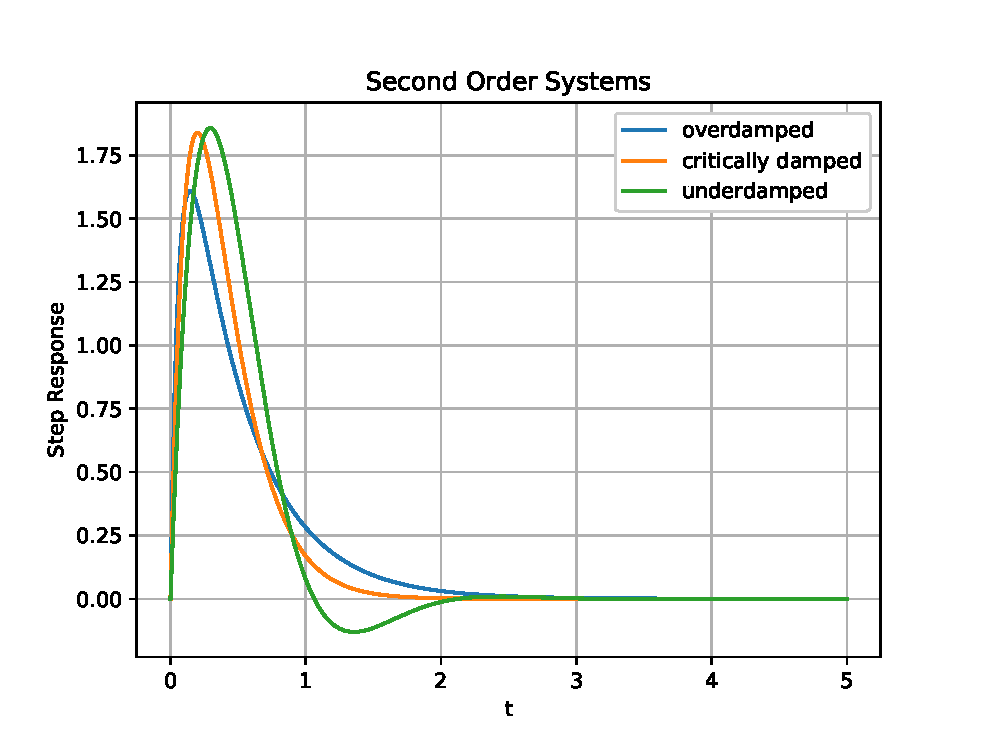
\includegraphics[width=\columnwidth]{./figs/ee18btech11012.eps}
%    \caption{}
%    \label{fig:ee18btech11012}
%\end{figure}

using a Python code to sketch the response.  
\end{enumerate}

\caption{}
\label{table:ee18btech11012}
\end{table}

\item Classify the following second-order systems according to damping.
\label{prob:ee18btech11012_damp}
\begin{enumerate}
\item $H(s) = \frac{15}{{s^2+5s+15}}$ 
\item $H(s) = \frac{25}{{s^2+10s+25}}$
\item $H(s) =\frac{35}{{s^2+18s+35}}$ 
\end{enumerate}
\solution For 
\begin{align}
H(s) &= \frac{25}{{s^2+10s+25}},
\\
     \omega^2 &= 25,   2\zeta\omega =10\\
\implies  \omega &=1,  {\zeta} = 1
\end{align}
and the system is critically damped.  Similarly, the damping factors for other systems in Problem \ref{prob:ee18btech11012_damp} are calculated and listed in Table \ref{table:ee18btech11012_damp}
%
\begin{table}[!ht]
\centering
%%%%%%%%%%%%%%%%%%%%%%%%%%%%%%%%%%%%%%%%%%%%%%%%%%%%%%%%%%%%%%%%%%%%%%
%%                                                                  %%
%%  This is the header of a LaTeX2e file exported from Gnumeric.    %%
%%                                                                  %%
%%  This file can be compiled as it stands or included in another   %%
%%  LaTeX document. The table is based on the longtable package so  %%
%%  the longtable options (headers, footers...) can be set in the   %%
%%  preamble section below (see PRAMBLE).                           %%
%%                                                                  %%
%%  To include the file in another, the following two lines must be %%
%%  in the including file:                                          %%
%%        \def\inputGnumericTable{}                                 %%
%%  at the beginning of the file and:                               %%
%%        \input{name-of-this-file.tex}                             %%
%%  where the table is to be placed. Note also that the including   %%
%%  file must use the following packages for the table to be        %%
%%  rendered correctly:                                             %%
%%    \usepackage[latin1]{inputenc}                                 %%
%%    \usepackage{color}                                            %%
%%    \usepackage{array}                                            %%
%%    \usepackage{longtable}                                        %%
%%    \usepackage{calc}                                             %%
%%    \usepackage{multirow}                                         %%
%%    \usepackage{hhline}                                           %%
%%    \usepackage{ifthen}                                           %%
%%  optionally (for landscape tables embedded in another document): %%
%%    \usepackage{lscape}                                           %%
%%                                                                  %%
%%%%%%%%%%%%%%%%%%%%%%%%%%%%%%%%%%%%%%%%%%%%%%%%%%%%%%%%%%%%%%%%%%%%%%



%%  This section checks if we are begin input into another file or  %%
%%  the file will be compiled alone. First use a macro taken from   %%
%%  the TeXbook ex 7.7 (suggestion of Han-Wen Nienhuys).            %%
\def\ifundefined#1{\expandafter\ifx\csname#1\endcsname\relax}


%%  Check for the \def token for inputed files. If it is not        %%
%%  defined, the file will be processed as a standalone and the     %%
%%  preamble will be used.                                          %%
\ifundefined{inputGnumericTable}

%%  We must be able to close or not the document at the end.        %%
	\def\gnumericTableEnd{\end{document}}


%%%%%%%%%%%%%%%%%%%%%%%%%%%%%%%%%%%%%%%%%%%%%%%%%%%%%%%%%%%%%%%%%%%%%%
%%                                                                  %%
%%  This is the PREAMBLE. Change these values to get the right      %%
%%  paper size and other niceties.                                  %%
%%                                                                  %%
%%%%%%%%%%%%%%%%%%%%%%%%%%%%%%%%%%%%%%%%%%%%%%%%%%%%%%%%%%%%%%%%%%%%%%

	\documentclass[12pt%
			  %,landscape%
                    ]{report}
       \usepackage[latin1]{inputenc}
       \usepackage{fullpage}
       \usepackage{color}
       \usepackage{array}
       \usepackage{longtable}
       \usepackage{calc}
       \usepackage{multirow}
       \usepackage{hhline}
       \usepackage{ifthen}

	\begin{document}


%%  End of the preamble for the standalone. The next section is for %%
%%  documents which are included into other LaTeX2e files.          %%
\else

%%  We are not a stand alone document. For a regular table, we will %%
%%  have no preamble and only define the closing to mean nothing.   %%
    \def\gnumericTableEnd{}

%%  If we want landscape mode in an embedded document, comment out  %%
%%  the line above and uncomment the two below. The table will      %%
%%  begin on a new page and run in landscape mode.                  %%
%       \def\gnumericTableEnd{\end{landscape}}
%       \begin{landscape}


%%  End of the else clause for this file being \input.              %%
\fi

%%%%%%%%%%%%%%%%%%%%%%%%%%%%%%%%%%%%%%%%%%%%%%%%%%%%%%%%%%%%%%%%%%%%%%
%%                                                                  %%
%%  The rest is the gnumeric table, except for the closing          %%
%%  statement. Changes below will alter the table's appearance.     %%
%%                                                                  %%
%%%%%%%%%%%%%%%%%%%%%%%%%%%%%%%%%%%%%%%%%%%%%%%%%%%%%%%%%%%%%%%%%%%%%%

\providecommand{\gnumericmathit}[1]{#1} 
%%  Uncomment the next line if you would like your numbers to be in %%
%%  italics if they are italizised in the gnumeric table.           %%
%\renewcommand{\gnumericmathit}[1]{\mathit{#1}}
\providecommand{\gnumericPB}[1]%
{\let\gnumericTemp=\\#1\let\\=\gnumericTemp\hspace{0pt}}
 \ifundefined{gnumericTableWidthDefined}
        \newlength{\gnumericTableWidth}
        \newlength{\gnumericTableWidthComplete}
        \newlength{\gnumericMultiRowLength}
        \global\def\gnumericTableWidthDefined{}
 \fi
%% The following setting protects this code from babel shorthands.  %%
 \ifthenelse{\isundefined{\languageshorthands}}{}{\languageshorthands{english}}
%%  The default table format retains the relative column widths of  %%
%%  gnumeric. They can easily be changed to c, r or l. In that case %%
%%  you may want to comment out the next line and uncomment the one %%
%%  thereafter                                                      %%
\providecommand\gnumbox{\makebox[0pt]}
%%\providecommand\gnumbox[1][]{\makebox}

%% to adjust positions in multirow situations                       %%
\setlength{\bigstrutjot}{\jot}
\setlength{\extrarowheight}{\doublerulesep}

%%  The \setlongtables command keeps column widths the same across  %%
%%  pages. Simply comment out next line for varying column widths.  %%
\setlongtables

\setlength\gnumericTableWidth{%
	36pt+%
	20pt+%
	35pt+%
	91pt+%
0pt}
\def\gumericNumCols{4}
\setlength\gnumericTableWidthComplete{\gnumericTableWidth+%
         \tabcolsep*\gumericNumCols*2+\arrayrulewidth*\gumericNumCols}
\ifthenelse{\lengthtest{\gnumericTableWidthComplete > \linewidth}}%
         {\def\gnumericScale{\ratio{\linewidth-%
                        \tabcolsep*\gumericNumCols*2-%
                        \arrayrulewidth*\gumericNumCols}%
{\gnumericTableWidth}}}%
{\def\gnumericScale{1}}

%%%%%%%%%%%%%%%%%%%%%%%%%%%%%%%%%%%%%%%%%%%%%%%%%%%%%%%%%%%%%%%%%%%%%%
%%                                                                  %%
%% The following are the widths of the various columns. We are      %%
%% defining them here because then they are easier to change.       %%
%% Depending on the cell formats we may use them more than once.    %%
%%                                                                  %%
%%%%%%%%%%%%%%%%%%%%%%%%%%%%%%%%%%%%%%%%%%%%%%%%%%%%%%%%%%%%%%%%%%%%%%

\ifthenelse{\isundefined{\gnumericColA}}{\newlength{\gnumericColA}}{}\settowidth{\gnumericColA}{\begin{tabular}{@{}p{36pt*\gnumericScale}@{}}x\end{tabular}}
\ifthenelse{\isundefined{\gnumericColB}}{\newlength{\gnumericColB}}{}\settowidth{\gnumericColB}{\begin{tabular}{@{}p{20pt*\gnumericScale}@{}}x\end{tabular}}
\ifthenelse{\isundefined{\gnumericColC}}{\newlength{\gnumericColC}}{}\settowidth{\gnumericColC}{\begin{tabular}{@{}p{35pt*\gnumericScale}@{}}x\end{tabular}}
\ifthenelse{\isundefined{\gnumericColD}}{\newlength{\gnumericColD}}{}\settowidth{\gnumericColD}{\begin{tabular}{@{}p{91pt*\gnumericScale}@{}}x\end{tabular}}

\begin{tabular}[c]{%
	b{\gnumericColA}%
	b{\gnumericColB}%
	b{\gnumericColC}%
	b{\gnumericColD}%
	}

%%%%%%%%%%%%%%%%%%%%%%%%%%%%%%%%%%%%%%%%%%%%%%%%%%%%%%%%%%%%%%%%%%%%%%
%%  The longtable options. (Caption, headers... see Goosens, p.124) %%
%	\caption{The Table Caption.}             \\	%
% \hline	% Across the top of the table.
%%  The rest of these options are table rows which are placed on    %%
%%  the first, last or every page. Use \multicolumn if you want.    %%

%%  Header for the first page.                                      %%
%	\multicolumn{4}{c}{The First Header} \\ \hline 
%	\multicolumn{1}{c}{colTag}	%Column 1
%	&\multicolumn{1}{c}{colTag}	%Column 2
%	&\multicolumn{1}{c}{colTag}	%Column 3
%	&\multicolumn{1}{c}{colTag}	\\ \hline %Last column
%	\endfirsthead

%%  The running header definition.                                  %%
%	\hline
%	\multicolumn{4}{l}{\ldots\small\slshape continued} \\ \hline
%	\multicolumn{1}{c}{colTag}	%Column 1
%	&\multicolumn{1}{c}{colTag}	%Column 2
%	&\multicolumn{1}{c}{colTag}	%Column 3
%	&\multicolumn{1}{c}{colTag}	\\ \hline %Last column
%	\endhead

%%  The running footer definition.                                  %%
%	\hline
%	\multicolumn{4}{r}{\small\slshape continued\ldots} \\
%	\endfoot

%%  The ending footer definition.                                   %%
%	\multicolumn{4}{c}{That's all folks} \\ \hline 
%	\endlastfoot
%%%%%%%%%%%%%%%%%%%%%%%%%%%%%%%%%%%%%%%%%%%%%%%%%%%%%%%%%%%%%%%%%%%%%%

\hhline{|-|-|-|-}
	 \multicolumn{1}{|p{\gnumericColA}|}%
	{\gnumericPB{\centering}\gnumbox{\textbf{H(s)}}}
	&\multicolumn{1}{p{\gnumericColB}|}%
	{\gnumericPB{\centering}\gnumbox{\textbf{$\omega$}}}
	&\multicolumn{1}{p{\gnumericColC}|}%
	{\gnumericPB{\centering}\gnumbox{\textbf{$\zeta$}}}
	&\multicolumn{1}{p{\gnumericColD}|}%
	{\gnumericPB{\raggedright}\gnumbox[l]{\textbf{Damping Type}}}
\\
\hhline{|----|}
	 \multicolumn{1}{|p{\gnumericColA}|}%
	{$\frac{35}{{s^2+18s+35}}$ }
	&\multicolumn{1}{p{\gnumericColB}|}%
	{$\sqrt{35}$}
	&\multicolumn{1}{p{\gnumericColC}|}%
	{\gnumericPB{\centering}\gnumbox{$\sqrt{\frac{81}{35}}> 1$}}
	&\multicolumn{1}{p{\gnumericColD}|}%
	{\gnumericPB{\raggedright}\gnumbox[l]{Overdamped}}
\\
\hhline{|----|}
	 \multicolumn{1}{|p{\gnumericColA}|}%
	{$\frac{25}{{s^2+10s+25}}$}
	&\multicolumn{1}{p{\gnumericColB}|}%
	{$5$}
	&\multicolumn{1}{p{\gnumericColC}|}%
	{\gnumericPB{\centering}\gnumbox{$1$}}
	&\multicolumn{1}{p{\gnumericColD}|}%
	{\gnumericPB{\raggedright}\gnumbox[l]{Critically Damped}}
\\
\hhline{|----|}
	 \multicolumn{1}{|p{\gnumericColA}|}%
	{$\frac{15}{{s^2+5s+15}}$}
	&\multicolumn{1}{p{\gnumericColB}|}%
	{$\sqrt{15}$}
	&\multicolumn{1}{p{\gnumericColC}|}%
	{\gnumericPB{\centering}\gnumbox{$\sqrt{\frac{5}{12}}< 1$}}
	&\multicolumn{1}{p{\gnumericColD}|}%
	{\gnumericPB{\raggedright}\gnumbox[l]{Underdamped}}
\\
\hhline{|-|-|-|-|}
\end{tabular}

\ifthenelse{\isundefined{\languageshorthands}}{}{\languageshorthands{\languagename}}
\gnumericTableEnd

\caption{}
\label{table:ee18btech11012_damp}
\end{table}

\item Find the step response of each $H(s)$ in Table \ref{table:ee18btech11012_damp}.
\\
\solution 
\begin{enumerate}
\item For 
\begin{align}
 H(s)=\frac{15}{s^2+5s+15},
\end{align}
%
the step response is
\begin{equation}
y(t)=25te^{-5t}u(t)
\label{eq:ee18btech11012_over}
\end{equation}
\item For 
%
\begin{align}
H(s)=\frac{25}{s^2+10s+25},
\end{align}
%
the step response is
\begin{equation}
y(t)=\frac{30}{\sqrt{35}}e^{\frac{-5t}{2}}\sin\brak{\frac{\sqrt{35}}{2}t}u(t)
\label{eq:ee18btech11012_critical}
\end{equation}
\item  For 

\begin{align}
H(s)=\frac{35}{s^2+18s+35},
\end{align}
the step response is
\begin{equation}
    y(t)=\frac{35}{2\sqrt{46}}\sbrak{e^{(-9+\sqrt{46})t}-e^{(-9-\sqrt{46})t}}u(t)
\label{eq:ee18btech11012_under}
\end{equation}
\end{enumerate}
\item Illustrate the effect of damping by plotting the step responses in \eqref{eq:ee18btech11012_over}-\eqref{eq:ee18btech11012_under}
\\
\solution The following code
\begin{lstlisting}
codes/ee18btech11012.py
\end{lstlisting}
%
plots the desired graphs in
Fig.     \ref{fig:ee18btech11012}. 
%
%\begin{figure}[ht!]
%    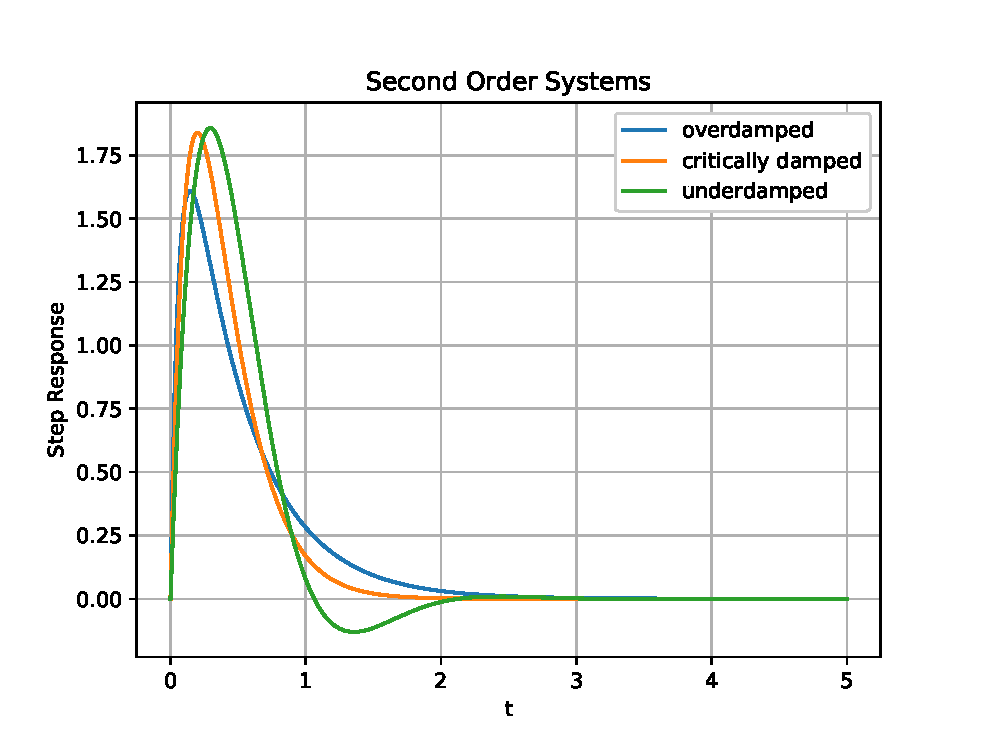
\includegraphics[width=\columnwidth]{./figs/ee18btech11012.eps}
%    \caption{}
%    \label{fig:ee18btech11012}
%\end{figure}

using a Python code to sketch the response.  
\end{enumerate}

%\begin{enumerate}[label=\thesubsection.\arabic*.,ref=\thesubsection.\theenumi]
%\numberwithin{equation}{enumi}
\item Sketch the polar plot of 
\begin{align}
    G(s) = \frac{1}{(s^2)(s+1)(s+2)}. 
    \label{eq:ee18btech11028_1}
\end{align}
%
\solution
Substituting $s = \j\omega$ in      \eqref{eq:ee18btech11028_1},

Now the magnitude will be
\begin{align}
   r &=  |G(\j\omega)| = \frac{1}{(\omega^2)(\sqrt{1 + \omega^2})(\sqrt{1+4\omega^2})}
    \label{eq:ee18btech11028_2}
\\
\theta &=\angle G(\j\omega)  = - \tan^{-1}(0) - \tan^{-1}(\omega) - \tan^{-1}(2\omega)
\\
     &= 180\degree - \tan^{-1}(\omega) - \tan^{-1}(2\omega)
    \label{eq:ee18btech11028_3}
\end{align}

The polar plot is the $\brak{r,\theta}$ plot for $\omega \in \brak{0,\infty}$.
The following python code generates  the polar plot in Fig. \ref{fig:ee18btech11028_fig1}
\begin{lstlisting}
    codes/ee18btech11028.py
\end{lstlisting}
\begin{figure}[!h]
\centering
    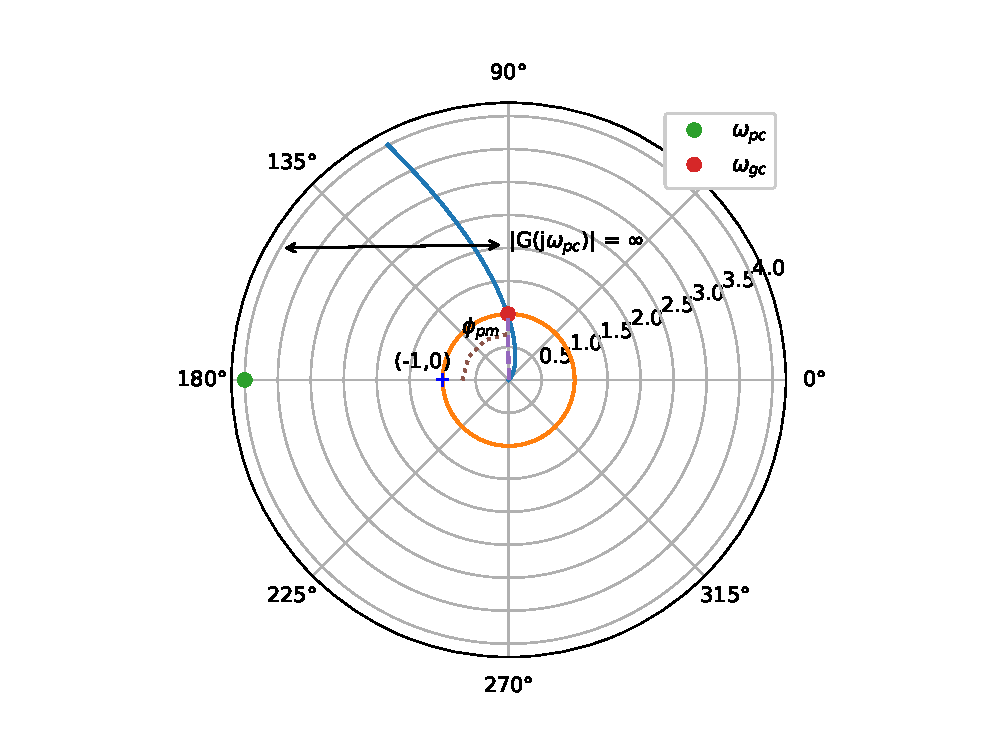
\includegraphics[width=\columnwidth]{./figs/ee18btech11028.eps}
  \caption{}
  \label{fig:ee18btech11028_fig1}
\end{figure}
The location of $\brak{-1,0}$ with respect to the polar plot provides information regarding the stability of the system.  
\begin{itemize}
    
    \item If  \brak{–1,0} is not enclosed, then it is stable.
    \item If \brak{–1,0} is enclosed by polar plot then it is unstable. 
    \item If \brak{–1,0} is on the polar plot then it is marginally stable
    
    
\end{itemize}
In Fig. \ref{fig:ee18btech11028_fig1},  the point \brak{-1,0} is enclosed by the polar plot,
which implies system is not stable.  The polar plot also provides info on the GM and PM, which can then be used for determining the stability of the system.

\begin{itemize}
    \item If the $GM > 1 \cap PM > 0$,  then the control system is \textbf{stable}.
    \item If the $GM = 1\cap PM =0 $,  then the control system is  \textbf{marginally stable}.
    \item If the $GM < 1\cup  PM < 0$ , then the control system is \textbf{unstable}.
\end{itemize}

Therefore, our system is unstable $\because GM < 1\cap  PM < 0$.



%\end{enumerate}

\begin{enumerate}[label=\thesubsection.\arabic*.,ref=\thesubsection.\theenumi]
\numberwithin{equation}{enumi}
\item
Sketch the Polar Plot of
\begin{align}
G\brak{s} = \frac{1}{s\brak{1+s^{2}}}
\label{eq:ee18btech11023_gain}
\end{align}
\\
\solution  From \eqref{eq:ee18btech11023_gain},

\begin{align}
G\brak{\j\omega} &=   \frac{1}{\j\omega\brak{1-{\omega}^{2}}}
\\
      \abs{G\brak{\j\omega}} &= \frac{1}{\abs{\omega\brak{1-{\omega}^{2}}}}
\\
    \angle G\brak{\j\omega} &= 
\begin{cases}
\frac{\pi}{2} & \omega > 1
\\
-\frac{\pi}{2} & 0 < \omega < 1
\end{cases}
    \end{align}
%
The corresponding polar plot is generated in Fig.   \ref{fig:ee18btech11023} using 
\begin{lstlisting}
codes/ee18btech11023.py
\end{lstlisting}

\begin{figure}[!ht]
\centering
  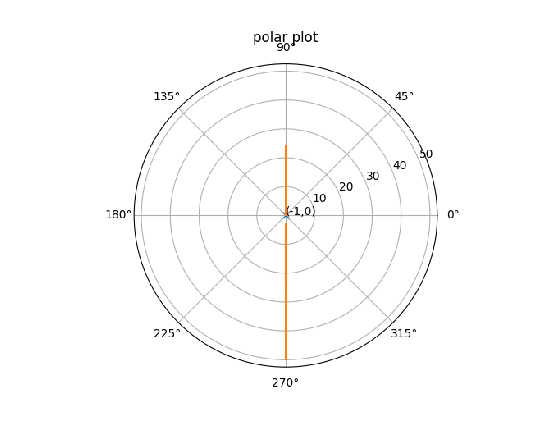
\includegraphics[width=\columnwidth]{./figs/ee18btech11023/ee18btech11023_1c.eps}
  \caption{}
  \label{fig:ee18btech11023}
\end{figure}
In Fig.   \ref{fig:ee18btech11023},  (–1,0) is exactly on the polar plot.  Hence, the system is marginally stable.


\end{enumerate}

%\begin{enumerate}[label=\thesubsection.\arabic*.,ref=\thesubsection.\theenumi]
%\numberwithin{equation}{enumi}
\item
Sketch the Polar Plot of
\begin{align}
G\brak{s} = \frac{\brak{1+\frac{s}{29}}\brak{1+0.0025s}}{\brak{s^{3}}\brak{1+0.005s}\brak{1+0.001s}}
\end{align}

\solution 
%
The following code generates the polar plot in Fig.   \ref{fig:ee18btech11029}

\begin{lstlisting}
codes/ee18btech11029.py
\end{lstlisting}

\begin{figure}[!h]
\centering
  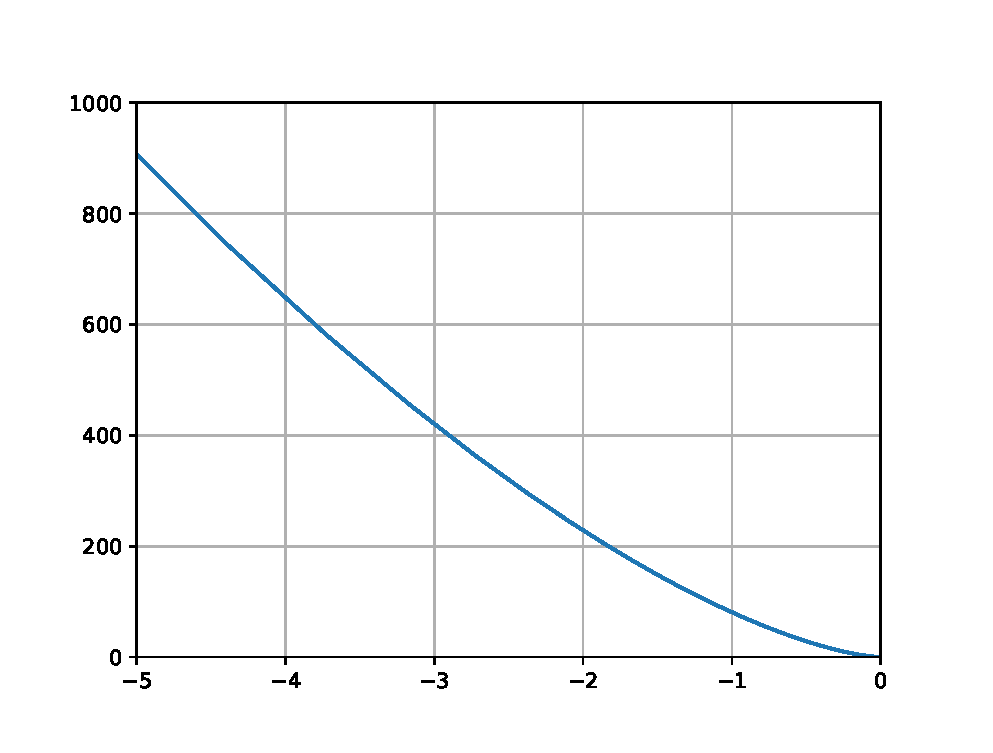
\includegraphics[width=\columnwidth]{./figs/ee18btech11029.eps}
  \caption{}
  \label{fig:ee18btech11029}
\end{figure}

\begin{itemize}
    \item The polar plots use open loop transfer function to determine the stability and hence reference point is shifted to \brak{-1,0}
    \item If \brak{–1,0} is left of the polar plot or \brak{–1,0} is not enclosed, then it is stable
    \item If \brak{–1,0} is on right side of the polar plot or \brak{–1,0} is enclosed by polar plot then it is unstable. 
    \item If \brak{–1,0} is on the polar plot then it is marginally stable
    
\end{itemize}

In Fig.   \ref{fig:ee18btech11029},  \brak{-1,0} is on the polar plot so the system is marginally stable.
   
%\end{enumerate}

\begin{enumerate}[label=\thesubsection.\arabic*.,ref=\thesubsection.\theenumi]
\numberwithin{equation}{enumi}
\item Plot the polar plot of 
\begin{align}
G(s) = \frac{1}{(s+1)(s+2)(s+3)}. 
\end{align}

\solution


\begin{figure}[!ht]
\centering
  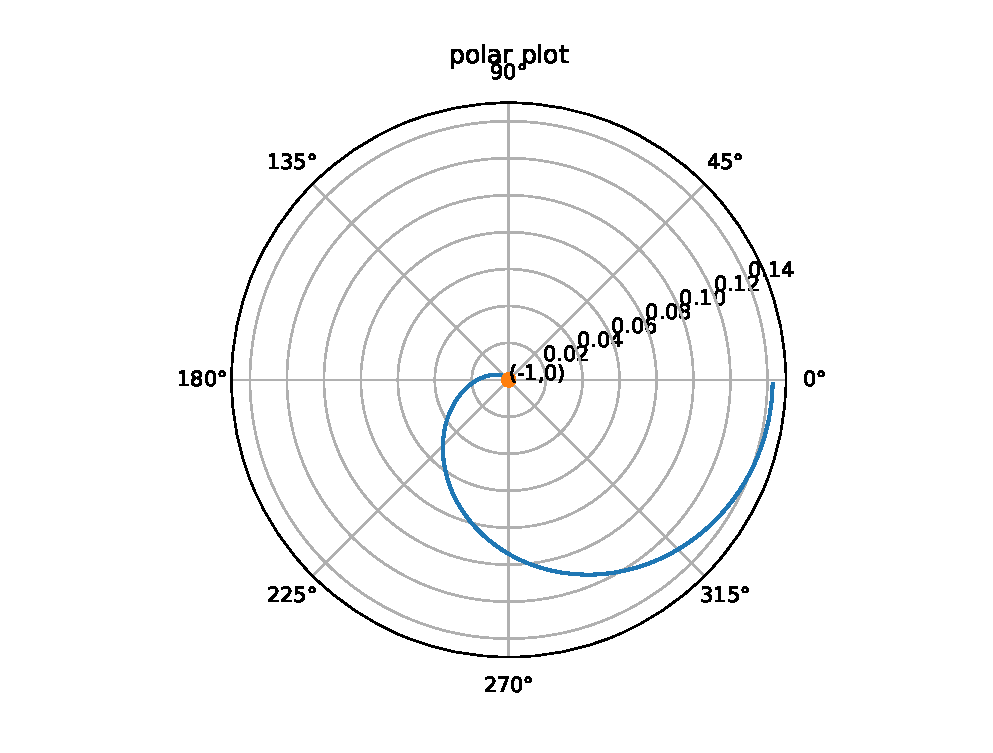
\includegraphics[width=\columnwidth]{./figs/ee18btech11033.eps}
\caption{}
  \label{fig:ee18btech11033}
  \label{fig:ee18btech11033}
\end{figure}

The following python code generates the polar plot in Fig.   \ref{fig:ee18btech11033}

\begin{lstlisting}
codes/ee18btech11033.py
\end{lstlisting}
$\because$  (-1,0) is on the right side of the polar plot, the system is unstable.

\end{enumerate}

%\begin{enumerate}[label=\thesection.\arabic*.,ref=\thesection.\theenumi]
%\numberwithin{equation}{enumi}
\item Plot the polar plot of 
\begin{align}
G(s) = \frac{100(s+5)}{s(s+3)(s^2+4)}. 
\end{align}

\solution
The following python code generates the polar plot in Fig.   \ref{fig:ee18btech11042_polarplot}

\begin{lstlisting}
codes/ee18btech11042.py
\end{lstlisting}

\begin{figure}[!ht]
\centering
  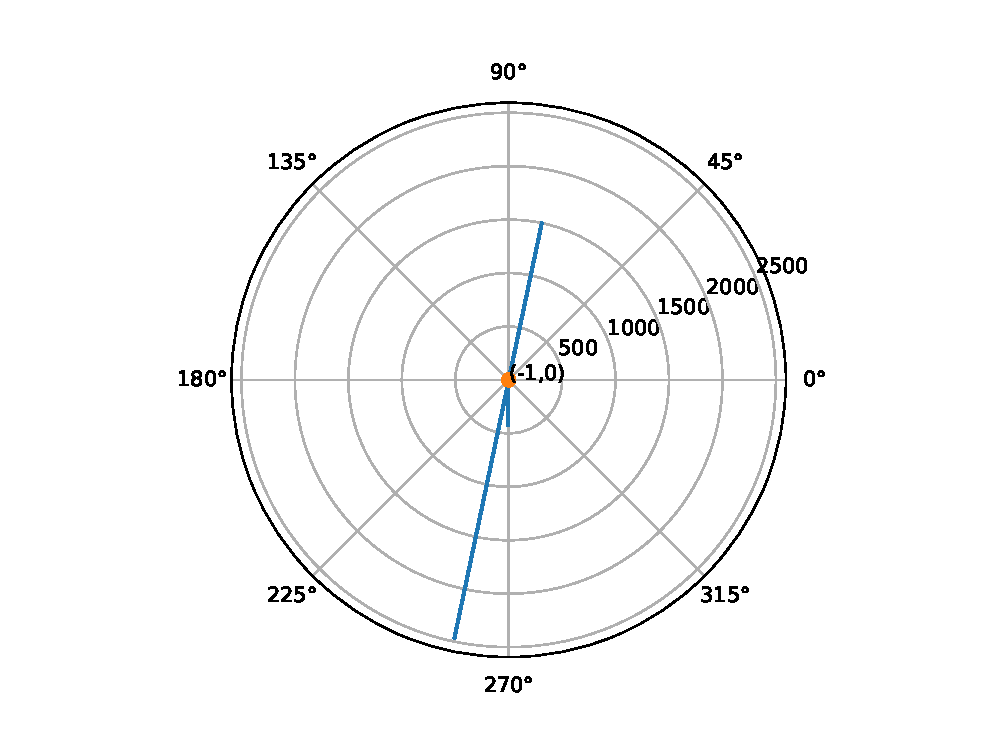
\includegraphics[width=\columnwidth]{./figs/ee18btech11042.eps}
\caption{}
  \label{fig:ee18btech11042_polarplot}
\end{figure}

Since (-1,0) is on the  polar plot, the  above system is  marginally stable.

%\end{enumerate}



\end{enumerate}
%
\subsection{Direct and Inverse Polar Plot}
\numberwithin{equation}{subsection}
%\begin{enumerate}[label=\thesection.\arabic*.,ref=\thesection.\theenumi]
%\numberwithin{equation}{enumi}
%\item 
Sketch the direct polar plot for a unity feedback system with open loop transfer function
\begin{align}
\label{eq:ee18btech11002_gain}
G(s) = \frac{1}{s(1+s)^2}
\end{align}
\\
\solution  
The polar plot is obtained by plotting $\brak{r,\phi}$
\begin{align}
r&=|H(\j\omega)||G(\j\omega)|
\\
\phi&=\angle H(\j\omega)G(\j\omega), 0 < \omega < \infty
\end{align}
The following code plots the polar plot in Fig. \ref{fig:ee18btech11002polar_plot}

\begin{lstlisting}
codes/ee18btech11002/polarplot.py
\end{lstlisting}
\begin{figure}[!ht]
\centering
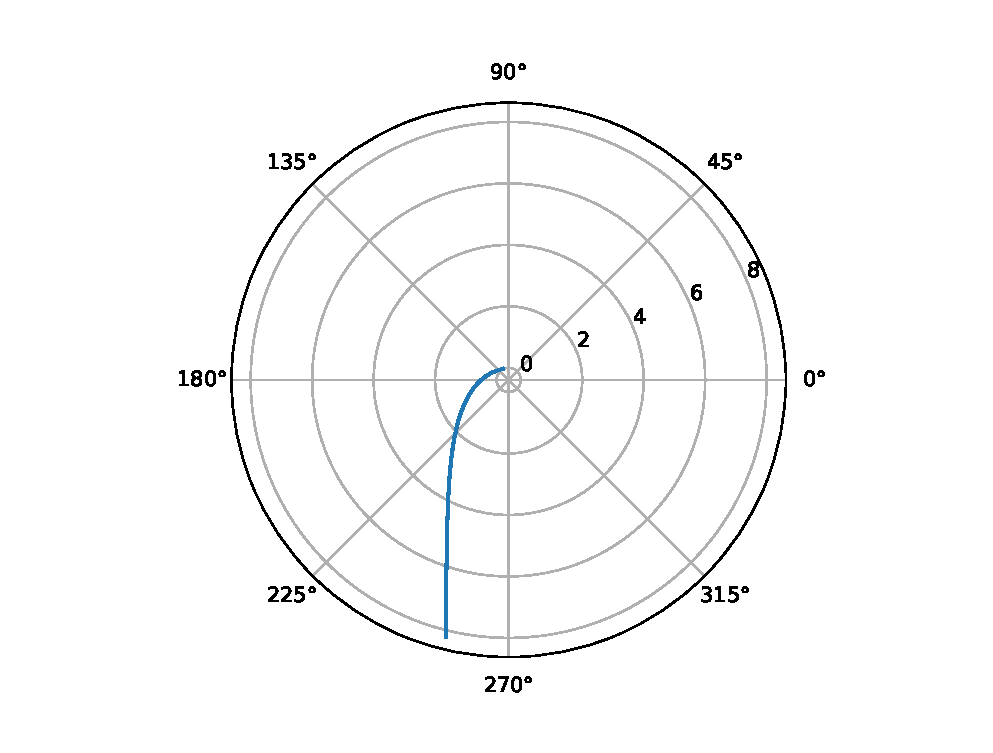
\includegraphics[width=\columnwidth]{./figs/ee18btech11002/ee18btech11002.eps}
\caption{Polar Plot}
\label{fig:ee18btech11002polar_plot}
\end{figure}
%\item 
Sketch the inverse polar plot for \eqref{eq:ee18btech11002_gain}
\\
\solution The above code plots the polar plot in Fig. \ref{fig:ee18btech11002inverse_polar_plot} by plotting  $\brak{\frac{1}{r}r,-\phi}$

%
\begin{figure}
\centering
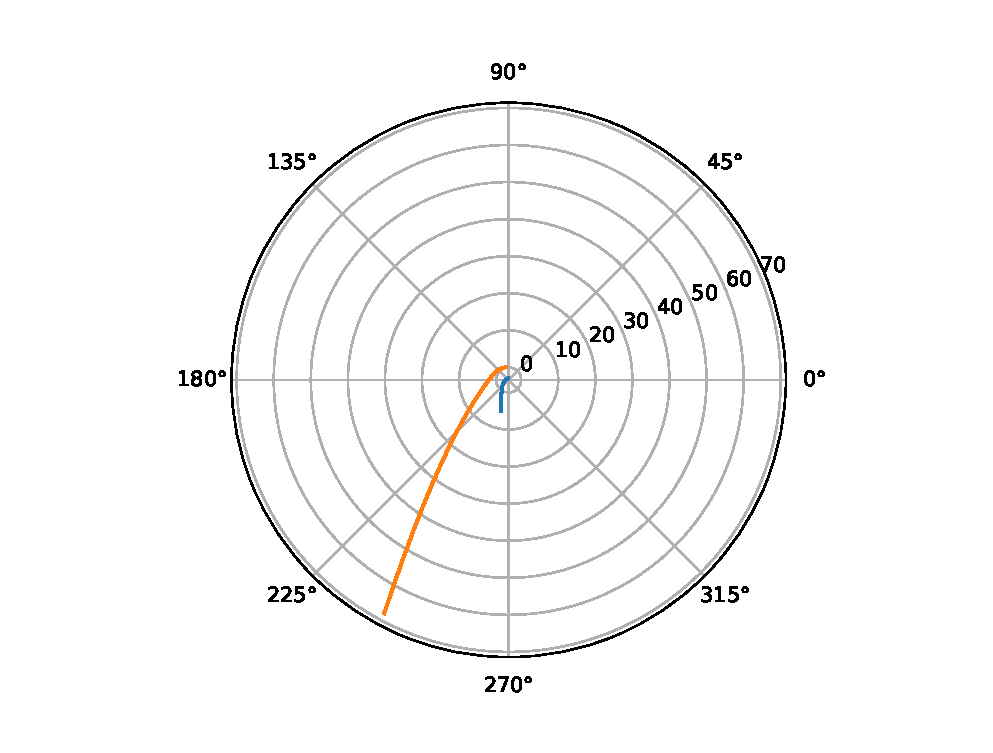
\includegraphics[width=\columnwidth]{./figs/ee18btech11002/ee18btech11002_1.eps}
\caption{Inverse Polar Plot}
\label{fig:ee18btech11002inverse_polar_plot}
\end{figure}


%\end{enumerate}


\subsection{Bode Plot}
\begin{enumerate}[label=\thesubsection.\arabic*.,ref=\thesubsection.\theenumi]
 
\begin{enumerate}[label=\thesection.\arabic*.,ref=\thesection.\theenumi]
\numberwithin{equation}{enumi}

\item Sketch the Bode Magnitude and Phase plot for the following system. Also compute the gain margin and the phase margin.
\begin{align}
G\brak{s} &= \frac{10}{s\brak{1+0.5s}\brak{1+.01s}}
\label{eq:ee18btech11048_2}
\end{align}
\\
\solution The Bode magnitude and phase plot are available in  Fig. \ref{fig:ee18btech11048} and generated by \begin{lstlisting}
codes/ee18btech11048.py
\end{lstlisting}

\begin{figure}[!h]
\centering
  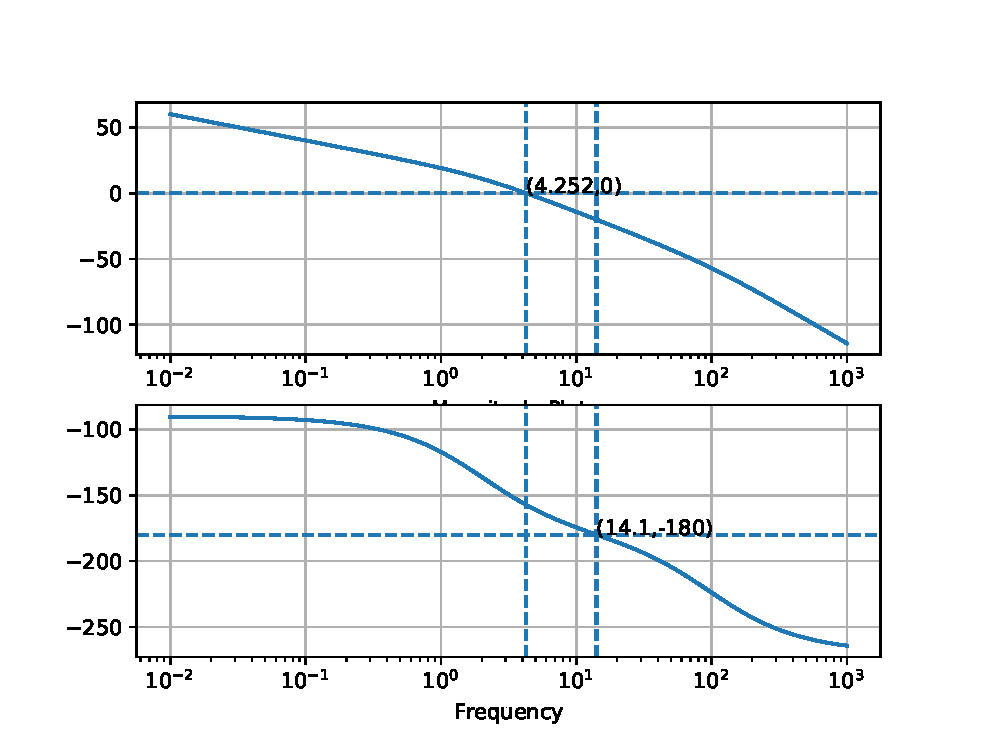
\includegraphics[width=\columnwidth]{./figs/ee18btech11048.eps}
  \caption{Graphs}
  \label{fig:ee18btech11048}
\end{figure}
The pole-zero locations are available in Table \ref{table:ee18btech11048}.
\begin{table}[!ht]
\centering
%%%%%%%%%%%%%%%%%%%%%%%%%%%%%%%%%%%%%%%%%%%%%%%%%%%%%%%%%%%%%%%%%%%%%%
%%                                                                  %%
%%  This is the header of a LaTeX2e file exported from Gnumeric.    %%
%%                                                                  %%
%%  This file can be compiled as it stands or included in another   %%
%%  LaTeX document. The table is based on the longtable package so  %%
%%  the longtable options (headers, footers...) can be set in the   %%
%%  preamble section below (see PRAMBLE).                           %%
%%                                                                  %%
%%  To include the file in another, the following two lines must be %%
%%  in the including file:                                          %%
%%        \def\inputGnumericTable{}                                 %%
%%  at the beginning of the file and:                               %%
%%        \input{name-of-this-file.tex}                             %%
%%  where the table is to be placed. Note also that the including   %%
%%  file must use the following packages for the table to be        %%
%%  rendered correctly:                                             %%
%%    \usepackage[latin1]{inputenc}                                 %%
%%    \usepackage{color}                                            %%
%%    \usepackage{array}                                            %%
%%    \usepackage{longtable}                                        %%
%%    \usepackage{calc}                                             %%
%%    \usepackage{multirow}                                         %%
%%    \usepackage{hhline}                                           %%
%%    \usepackage{ifthen}                                           %%
%%  optionally (for landscape tables embedded in another document): %%
%%    \usepackage{lscape}                                           %%
%%                                                                  %%
%%%%%%%%%%%%%%%%%%%%%%%%%%%%%%%%%%%%%%%%%%%%%%%%%%%%%%%%%%%%%%%%%%%%%%



%%  This section checks if we are begin input into another file or  %%
%%  the file will be compiled alone. First use a macro taken from   %%
%%  the TeXbook ex 7.7 (suggestion of Han-Wen Nienhuys).            %%
\def\ifundefined#1{\expandafter\ifx\csname#1\endcsname\relax}


%%  Check for the \def token for inputed files. If it is not        %%
%%  defined, the file will be processed as a standalone and the     %%
%%  preamble will be used.                                          %%
\ifundefined{inputGnumericTable}

%%  We must be able to close or not the document at the end.        %%
	\def\gnumericTableEnd{\end{document}}


%%%%%%%%%%%%%%%%%%%%%%%%%%%%%%%%%%%%%%%%%%%%%%%%%%%%%%%%%%%%%%%%%%%%%%
%%                                                                  %%
%%  This is the PREAMBLE. Change these values to get the right      %%
%%  paper size and other niceties.                                  %%
%%                                                                  %%
%%%%%%%%%%%%%%%%%%%%%%%%%%%%%%%%%%%%%%%%%%%%%%%%%%%%%%%%%%%%%%%%%%%%%%

	\documentclass[12pt%
			  %,landscape%
                    ]{report}
       \usepackage[latin1]{inputenc}
       \usepackage{fullpage}
       \usepackage{color}
       \usepackage{array}
       \usepackage{longtable}
       \usepackage{calc}
       \usepackage{multirow}
       \usepackage{hhline}
       \usepackage{ifthen}

	\begin{document}


%%  End of the preamble for the standalone. The next section is for %%
%%  documents which are included into other LaTeX2e files.          %%
\else

%%  We are not a stand alone document. For a regular table, we will %%
%%  have no preamble and only define the closing to mean nothing.   %%
    \def\gnumericTableEnd{}

%%  If we want landscape mode in an embedded document, comment out  %%
%%  the line above and uncomment the two below. The table will      %%
%%  begin on a new page and run in landscape mode.                  %%
%       \def\gnumericTableEnd{\end{landscape}}
%       \begin{landscape}


%%  End of the else clause for this file being \input.              %%
\fi

%%%%%%%%%%%%%%%%%%%%%%%%%%%%%%%%%%%%%%%%%%%%%%%%%%%%%%%%%%%%%%%%%%%%%%
%%                                                                  %%
%%  The rest is the gnumeric table, except for the closing          %%
%%  statement. Changes below will alter the table's appearance.     %%
%%                                                                  %%
%%%%%%%%%%%%%%%%%%%%%%%%%%%%%%%%%%%%%%%%%%%%%%%%%%%%%%%%%%%%%%%%%%%%%%

\providecommand{\gnumericmathit}[1]{#1} 
%%  Uncomment the next line if you would like your numbers to be in %%
%%  italics if they are italizised in the gnumeric table.           %%
%\renewcommand{\gnumericmathit}[1]{\mathit{#1}}
\providecommand{\gnumericPB}[1]%
{\let\gnumericTemp=\\#1\let\\=\gnumericTemp\hspace{0pt}}
 \ifundefined{gnumericTableWidthDefined}
        \newlength{\gnumericTableWidth}
        \newlength{\gnumericTableWidthComplete}
        \newlength{\gnumericMultiRowLength}
        \global\def\gnumericTableWidthDefined{}
 \fi
%% The following setting protects this code from babel shorthands.  %%
 \ifthenelse{\isundefined{\languageshorthands}}{}{\languageshorthands{english}}
%%  The default table format retains the relative column widths of  %%
%%  gnumeric. They can easily be changed to c, r or l. In that case %%
%%  you may want to comment out the next line and uncomment the one %%
%%  thereafter                                                      %%
\providecommand\gnumbox{\makebox[0pt]}
%%\providecommand\gnumbox[1][]{\makebox}

%% to adjust positions in multirow situations                       %%
\setlength{\bigstrutjot}{\jot}
\setlength{\extrarowheight}{\doublerulesep}

%%  The \setlongtables command keeps column widths the same across  %%
%%  pages. Simply comment out next line for varying column widths.  %%
\setlongtables

\setlength\gnumericTableWidth{%
	55pt+%
	35pt+%
	119pt+%
0pt}
\def\gumericNumCols{3}
\setlength\gnumericTableWidthComplete{\gnumericTableWidth+%
         \tabcolsep*\gumericNumCols*2+\arrayrulewidth*\gumericNumCols}
\ifthenelse{\lengthtest{\gnumericTableWidthComplete > \linewidth}}%
         {\def\gnumericScale{\ratio{\linewidth-%
                        \tabcolsep*\gumericNumCols*2-%
                        \arrayrulewidth*\gumericNumCols}%
{\gnumericTableWidth}}}%
{\def\gnumericScale{1}}

%%%%%%%%%%%%%%%%%%%%%%%%%%%%%%%%%%%%%%%%%%%%%%%%%%%%%%%%%%%%%%%%%%%%%%
%%                                                                  %%
%% The following are the widths of the various columns. We are      %%
%% defining them here because then they are easier to change.       %%
%% Depending on the cell formats we may use them more than once.    %%
%%                                                                  %%
%%%%%%%%%%%%%%%%%%%%%%%%%%%%%%%%%%%%%%%%%%%%%%%%%%%%%%%%%%%%%%%%%%%%%%

\ifthenelse{\isundefined{\gnumericColA}}{\newlength{\gnumericColA}}{}\settowidth{\gnumericColA}{\begin{tabular}{@{}p{55pt*\gnumericScale}@{}}x\end{tabular}}
\ifthenelse{\isundefined{\gnumericColB}}{\newlength{\gnumericColB}}{}\settowidth{\gnumericColB}{\begin{tabular}{@{}p{35pt*\gnumericScale}@{}}x\end{tabular}}
\ifthenelse{\isundefined{\gnumericColC}}{\newlength{\gnumericColC}}{}\settowidth{\gnumericColC}{\begin{tabular}{@{}p{119pt*\gnumericScale}@{}}x\end{tabular}}

\begin{tabular}[c]{%
	b{\gnumericColA}%
	b{\gnumericColB}%
	b{\gnumericColC}%
	}

%%%%%%%%%%%%%%%%%%%%%%%%%%%%%%%%%%%%%%%%%%%%%%%%%%%%%%%%%%%%%%%%%%%%%%
%%  The longtable options. (Caption, headers... see Goosens, p.124) %%
%	\caption{The Table Caption.}             \\	%
% \hline	% Across the top of the table.
%%  The rest of these options are table rows which are placed on    %%
%%  the first, last or every page. Use \multicolumn if you want.    %%

%%  Header for the first page.                                      %%
%	\multicolumn{3}{c}{The First Header} \\ \hline 
%	\multicolumn{1}{c}{colTag}	%Column 1
%	&\multicolumn{1}{c}{colTag}	%Column 2
%	&\multicolumn{1}{c}{colTag}	\\ \hline %Last column
%	\endfirsthead

%%  The running header definition.                                  %%
%	\hline
%	\multicolumn{3}{l}{\ldots\small\slshape continued} \\ \hline
%	\multicolumn{1}{c}{colTag}	%Column 1
%	&\multicolumn{1}{c}{colTag}	%Column 2
%	&\multicolumn{1}{c}{colTag}	\\ \hline %Last column
%	\endhead

%%  The running footer definition.                                  %%
%	\hline
%	\multicolumn{3}{r}{\small\slshape continued\ldots} \\
%	\endfoot

%%  The ending footer definition.                                   %%
%	\multicolumn{3}{c}{That's all folks} \\ \hline 
%	\endlastfoot
%%%%%%%%%%%%%%%%%%%%%%%%%%%%%%%%%%%%%%%%%%%%%%%%%%%%%%%%%%%%%%%%%%%%%%

\hhline{|-|-}
	 \multicolumn{1}{|p{\gnumericColA}|}%
	{\gnumericPB{\centering}\textbf{Zeros}}
	&\multicolumn{1}{p{\gnumericColB}|}%
	{\gnumericPB{\centering}\textbf{Poles}}

\\
\hhline{|---|}
	 \multicolumn{1}{|p{\gnumericColA}|}%
	{\gnumericPB{\centering}-}
	&\multicolumn{1}{p{\gnumericColB}|}%
	{\gnumericPB{\centering}0}

\\
\hhline{|---|}
	 \multicolumn{1}{|p{\gnumericColA}|}%
	{\gnumericPB{\centering} }
	&\multicolumn{1}{p{\gnumericColB}|}%
	{\gnumericPB{\centering}-2}

\\
\hhline{|---|}
	 \multicolumn{1}{|p{\gnumericColA}|}%
	{\gnumericPB{\centering} }
	&\multicolumn{1}{p{\gnumericColB}|}%
	{\gnumericPB{\centering}-100}

\\
\hhline{|-|-|-|}
\end{tabular}

\ifthenelse{\isundefined{\languageshorthands}}{}{\languageshorthands{\languagename}}
\gnumericTableEnd

\caption{Zeros and Poles}
\label{table:ee18btech11048}
\end{table}



The  {\em Gain} and {\em Phase} of \eqref{eq:ee18btech11048_2} are
\begin{align}
\abs{G\brak{\j\omega}}  =  \frac{100}{\omega\sqrt{\brak{0.5\omega}^2+1}\sqrt{\brak{0.01\omega}^2+1}}
\label{eq:ee18btech11048_2}
\end{align}
\begin{multline}
\phase{G\brak{\j\omega}}  =  \tan^{-1} \brak{0}-\tan^{-1} \brak{\frac{\omega}{0}} - \tan^{-1} \brak{\frac{\omega}{2}}- \\\tan^{-1} \brak{\frac{\omega}{100}} 
\label{eq:ee18btech11048_3}
\end{multline}
Hence, 
\begin{align}
\abs{G\brak{\j\omega_{gc}}}  &=  1
\\
\implies \omega_{gc} &= 4.25  
\\
\phase{ G\brak{\j\omega_{gc}}} &= -157.2 \\
\implies PM &= 22.8 
\end{align}
%
Similarly, 
\begin{align}
\phase{G\brak{\j\omega_{pc}}}  &= -180\degree
\\
\implies
\omega_{pc} &=  14.1 \\
\implies -\abs{G\brak{\j\omega_{pc}}}  &= -20.2 dB \\
\implies
GM &= 20.2 dB
\end{align}

\end{enumerate}

%\begin{enumerate}[label=\thesection.\arabic*.,ref=\thesection.\theenumi]
%\numberwithin{equation}{enumi}

\item Plot the Bode magnitude and phase plots for the following system
\begin{align}
G\brak{s} &= \frac{75\brak{1+0.2s}}{s\brak{s^2+16s+100}}
\label{eq:ee18btech11049_system}
\end{align}
Also compute gain margin and phase margin .
\\
\solution From  \eqref{eq:ee18btech11049_system}, we have 

\begin{align}
G\brak{\j\omega}&=\frac{75\brak{1+0.2\j\omega}}{\j\omega\brak{\brak{\j\omega}^2 + 16\j\omega+100} }
\end{align}
poles = 0 , -8-6j , -8+6j\\
zeros = -5\\
Gain and phase plots are shown in Fig.  \ref{fig:ee18btech11049} 
\begin{figure}[!h]
\centering
  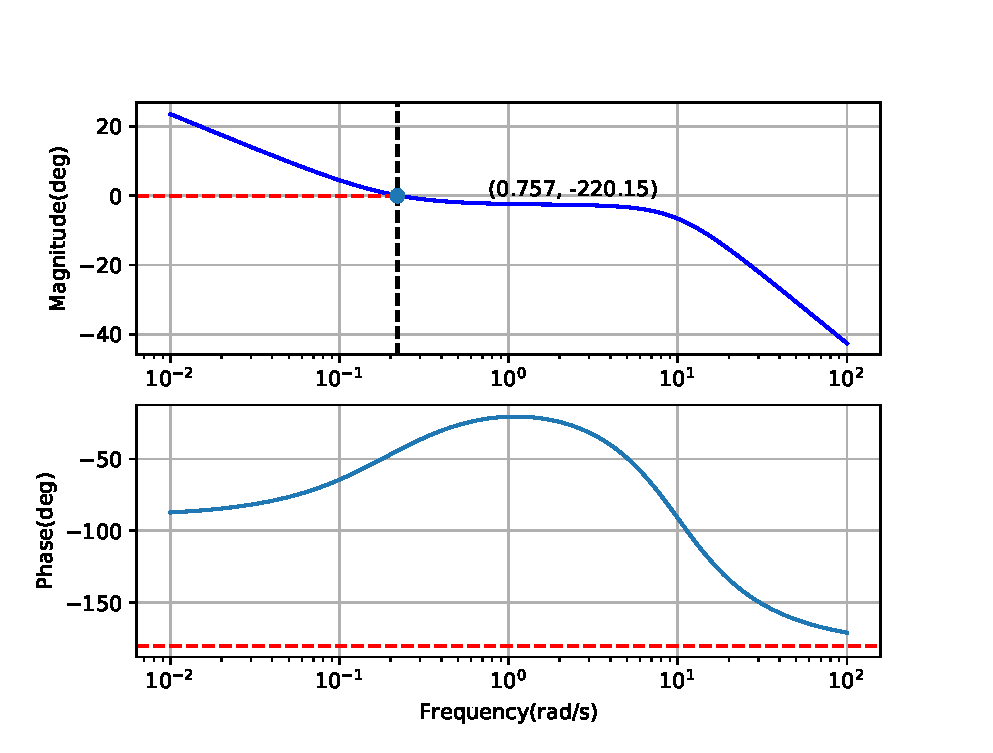
\includegraphics[width=\columnwidth]{./figs/ee18btech11049.eps}
  \caption{a}
  \label{fig:ee18btech11049}
\end{figure}

The following code plots Fig. \ref{fig:ee18btech11049} 

\begin{lstlisting}
codes/ee18btech11049.py
\end{lstlisting}

%\item Find $\phase G\brak{\j\omega} + 180\degree$ , where $\omega$ is frequency when gain = 1 . This is known as  {\em phase margin} (PM)
%\\
%\solution 
Solving 
\begin{align}
\label{eq:ee18btech11049_gain}
\begin{split}
\abs{G\brak{\j\omega}} &=   \frac{75\sqrt{\omega^2 + 25}}{\omega\sqrt{\brak{\omega+6}^2+64}\sqrt{\brak{\omega-6}^2+64}} 
\\
&= 1,
\end{split}
\end{align}
or from Fig. \ref{fig:ee18btech11049}, the gain crossover frequency 
%
\begin{align}
\implies
\omega_{gc} &=  0.757  \\
\phase{G\brak{\j\omega_{gc}}} &= -88.3 \\
\implies
PM &= 91.7  
% \label{eq:ee18btech11049_phase}
\end{align}

%\item Find $-G\brak{\j\omega}  $ db , where $\omega$ is frequency when phase = $-180\degree$ . This is known as  {\em gain margin} (GM)
%\\
\solution From Fig. \ref{fig:ee18btech11049} ,we can say that phase  never crosses $-180\degree$ .
So , the gain margin is {\em infinite}.
Which means we can add any gain, and the equivalent closed loop system never becomes unstable.

%\end{enumerate}

For the circuit shown in Fig. \ref{fig:es17btech11002_fig1}, find the loop gain $L(s) = G(s)H(s)$, $L\brak{\j\omega}$, the frequency for zero loop phase, and $R_{2}/R_{1}$ for oscillation.
\begin{enumerate}[label=\arabic*.,ref=\theenumi]
\numberwithin{equation}{enumi}
\item Draw the equivalent control system representation for the circuit in Fig. \ref{fig:es17btech11002_fig1} as well as the small signal model. 
\\
\solution See Figs. \ref{fig:es17btech11002_block}, \ref{fig:es17btech11002_fig2} and \ref{fig:es17btech11002_fig3}. Oscillators do not include input signal.
%
\renewcommand{\thefigure}{\theenumi.\arabic{figure}}
%
\begin{figure}[!ht]
	\begin{center}
		\resizebox{\columnwidth}{!}{\begin{circuitikz}
\ctikzset{bipoles/length=1cm}

 
\draw (0, 0) node[op amp] (opamp) {};
\draw (opamp.-) --(-1,0.35)-- (-1,1) to[R=$R_2$,*-*] (1,1) -- (1,0) -- (1,-1) to [R=$R$,*-*] (0.25,-1) to [C=$C$,*-*] (-1,-1) -- (-1,-0.35) to (opamp.+);
\draw (-1,1) to[R=$R_1$,*-*] (-5, 1) to node[ground]{}  (-5, 0.9) ;
\draw (0.25,-1) to [C = $C$,*-*] (0.25,-3) to node[ground]{} (0.25,-3);
\draw (-1,-1) to[R=$R$,*-*] (-1, -3) to node[ground]{} (-1,-3);
\draw (opamp.out) -- (1,0) ;
\draw node at (-1.3,0.35){$V_{f2}$};
\draw node at (-1.3,-0.35){$V_{f}$};
\end{circuitikz}
}
	\end{center}
\caption{}
\label{fig:es17btech11002_fig1}
\end{figure}
%
\begin{figure}[!ht]
	\begin{center}
		\resizebox{\columnwidth}{!}{
\tikzstyle{block} = [draw, fill=blue!20, rectangle,
    minimum height=3em, minimum width=4em]
\tikzstyle{sum} = [draw, fill=blue!20, circle, node distance=1cm]
\tikzstyle{input} = [coordinate]
\tikzstyle{output} = [coordinate]
\tikzstyle{out} = [coordinate]
\tikzstyle{pinstyle} = [pin edge={to-,thin,black}]
\begin{tikzpicture}[auto, node distance=2cm]
    \node [input, name=input] {};
    \node [sum, right of=input] (sum) {};
    \node [block, right of=sum] (controller) {$G_o$};
    \node [block, above of= controller](feedback2){$G_1$};
    \node [output, right of=controller] (output) {};
    \node [right of=output](out){$V_{o}$};
    \node [block, below of=controller] (feedback) {$H$};
    \draw [draw,->] (input) -- node {} (sum);
    \draw [->] (sum) -- node {} (controller);
    \draw [-] (controller) -- node {}(output);
    \draw [->] (output) |- (feedback);
    \draw [->] (output) |- (feedback2);
     \draw [->] (output) |- node{}(out);
     \draw [->] (feedback2) -| node[pos=0.99]{$-$}  node [near end] {$V_{f2}$} (sum);
    \draw [->] (feedback) -| node[pos=0.99]{$+$}  node [near end] {$V_f$} (sum);
\end{tikzpicture}
}
	\end{center}
\caption{Block diagram}
\label{fig:es17btech11002_block}
\end{figure}
\begin{figure}[!ht]
	\begin{center}
		\resizebox{\columnwidth}{!}{\tikzstyle{block} = [draw, fill=blue!20, rectangle, 
    minimum height=3em, minimum width=6em]
\tikzstyle{sum} = [draw, fill=blue!20, circle, node distance=1cm]
\tikzstyle{input} = [coordinate]
\tikzstyle{output} = [coordinate]
\tikzstyle{pinstyle} = [pin edge={to-,thin,black}]

\begin{tikzpicture}[auto, node distance=2cm,>=latex']
    \node [input, name=input] {};
    \node [sum, right of=input] (sum) {};
    \node [block, right of=sum] (controller) {$G$};
    \node [output, right of=controller] (output) {};
    \node [block, below of=controller] (feedback) {$H$};
    \draw [draw,->] (input) -- node {} (sum);
    \draw [->] (sum) -- node {$V_i$} (controller);
    \draw [->] (controller) -- node [name=y] {$V_o$}(output);
    \draw [->] (y) |- (feedback);
    \draw [->] (feedback) -| node[pos=0.99]{$+$}  node [near end] {$V_f$} (sum);
\end{tikzpicture}
}
	\end{center}
\caption{Simplified equivalent block diagram}
\label{fig:es17btech11002_fig2}
\end{figure}
%
\begin{figure}[!ht]
	\begin{center}
		\resizebox{\columnwidth}{!}{\usetikzlibrary{decorations.markings}
\begin{circuitikz}
\ctikzset{bipoles/length=1cm}

\draw 
(1.5,1) to [R=$R$] (1.5,5) to (1.5,5)  node[ground,rotate=180]{} 
(1.5,2) to [C=$C$] (3.5,2) to [C=$C$,*-*] (3.5,4) to (3.5,5) node[ground,rotate=180]{} 
(3.5,2) to [R=$R$] (5,2) -- (5,1)
%(1.5,3) node[pos=10]{$V_i$}
(1.5,-1.25)  node at(1.7,-1.25){$-$} 
(1.5,-1.25) -- (1,-1.25) -- (1,-1.75) to[R=$R_1$] (1,-2.75) --(1,-3) node[ground]{}
(1,-1.5) to[R=$R_2$,*-*] (5,-1.5) {}
(5,-1.5) -- (5,1) --(3.5,1) to[V=$G_{0}V_i$] (3.5,-0.5) node[ground]{}
(5,1) --(6,1)
(6,1) --(6.5,1) node at(6.8,1){$V_o$}
node at (1.8,-0.3) {$V_i$}
node at (3.5,1.7) {$V_{a}$}
node at (1.1,2) {$V_{f}$}
node at (0.65,-1.5){$V_{f2}$}
node at(1.8,1){$+$}
;\end{circuitikz}
}
	\end{center}
\caption{}
\label{fig:es17btech11002_fig3}
\end{figure}
\renewcommand{\thefigure}{\theenumi}
%
\item Draw the block diagram and circuit diagram for $H$.\\
\solution See Figs. \ref{fig:es17btech11002_fig4} and \ref{fig:es17btech11002_fig5}. 
\numberwithin{figure}{enumi}
\renewcommand{\thefigure}{\theenumi.\arabic{figure}}
\begin{figure}[!ht]
	\begin{center}
		\resizebox{\columnwidth}{!}{\begin{circuitikz}[american]
\usetikzlibrary{positioning, fit, calc}
\draw (0,0)to [open,v=$V_f$]++(0,-2)to[short]++(6,0)
(0,0)to++(6,0);
\draw (8,-1)node[draw,minimum width=4cm,minimum height=4cm] (load) {H}(8,0)
(10,0)--++(6,0)
(10,-2)--(16,-2)
node at (16,-1.7) {$-$}
node at (16,-0.3){$+$}
node at (16,-1){$V_o$}
;
\end{circuitikz}
}
	\end{center}
\caption{Feedback block diagram}
\label{fig:es17btech11002_fig4}
\end{figure}
\begin{figure}[!ht]
	\begin{center}
		\resizebox{\columnwidth}{!}{\begin{circuitikz}
\ctikzset{bipoles/length=1cm}

\draw (0,0) to [C=$C$,*-*] (2,0) to [R=$R$,*-*] (3,0);
\draw (0.5,0) to [R=$R$](0.5,-2) to node[ground]{} (0.5,-2);
\draw (2,0) to [C=$C$](2,-2) to node[ground]{} (2,-2);
\draw node at (-0.3,0) {$V_f$};
\draw node at (3.3,0) {$V_o$};
\end{circuitikz}

}
	\end{center}
\caption{Feedback circuit}
\label{fig:es17btech11002_fig5}
\end{figure}
\renewcommand{\thefigure}{\theenumi}
\item Find $H$.
\\
\solution In Fig. \ref{fig:es17btech11002_fig5}, let $I_o$ be the current flowing from $V_o$.  Then
\begin{align}
\label{eq:es17btech11002_H_io}
I_o = \frac{V_o}{R + \frac{1}{sC} \parallel \brak{\frac{1}{sC}+R}}
\end{align}
%
Using current division,
\begin{align}
\label{eq:es17btech11002_H_vf}
V_f = I_o \frac{\frac{1}{sC}}{\frac{1}{sC} +  \brak{\frac{1}{sC}+R}} \times R
\end{align}
From \eqref{eq:es17btech11002_H_io} and \eqref{eq:es17btech11002_H_vf},

\begin{align}
\frac{V_{f}}{V_{o}} &=\frac{\frac{1}{sC}}{\frac{1}{sC} +  \brak{\frac{1}{sC}+R}}\times R\\\
&\quad \times  \frac{1}{R + \frac{1}{sC} \parallel \brak{\frac{1}{sC}+R}}
\end{align}
On further simplification we get,
\begin{align}
\implies H &= \frac{1}{\brak{3+sRC +\frac{1}{sRC}}}
\label{eq:es17btech11002_H}
\end{align}
%
\item Find $R_{11}$ and $R_{22}$ from Fig. \ref{fig:es17btech11002_fig5}. 
\\
\solution Shorting  $V_{o}$ to ground,
\begin{align}
R_{11} &= R\parallel \brak{\frac{1}{sC}+ \frac{1}{sC}\parallel R} 
\label{eq:es17btech11002_6}
\end{align}
Shorting $V_{f}$ to ground,
\begin{align}
R_{22} &= \frac{1}{2sC} + R  
\end{align}
%
%----------------------------------------------------
\item Draw the block diagram and circuit diagram for $G$.\\
\solution See Figs. \ref{fig:es17btech11002_fig6} for the block diagram  and Figs. \ref{fig:es17btech11002_fig7} for the circuit diagram.
\numberwithin{figure}{enumi}
\renewcommand{\thefigure}{\theenumi.\arabic{figure}}
%
\begin{figure}[!ht]
	\begin{center}
		\resizebox{\columnwidth}{!}{\begin{circuitikz}[american]
\usetikzlibrary{positioning, fit, calc}
\draw (0,0)to [open,v=$V_i$]++(0,-2)to[short]++(6,0)
(0,0)to++(6,0);
\draw (8,-1)node[draw,minimum width=4cm,minimum height=4cm] (load) {G}(8,0)
(10,0) -- (16,0)
(3,0) to [R=$R_{11}$](3,-2)
(10,-2) to [R=$R_{22}$](16,-2)
node at (16,-1.7) {$-$}
node at (16,-0.3){$+$}
node at (16,-1){$V_o$}
;
\end{circuitikz}
}
	\end{center}
\caption{Open loop block diagram}
\label{fig:es17btech11002_fig6}
\end{figure}
%
\begin{figure}[!ht]
	\begin{center}
		\resizebox{\columnwidth}{!}{\usetikzlibrary{decorations.markings}
\begin{circuitikz}
\ctikzset{bipoles/length=1cm}

\draw 
(1.5,1)  to [R=$R_{11}$,*-*] (0,1) to (0,-1)  node[ground]{} 
%(1.5,2) to [R=$R$] (3,2) to [R=$R$] (3,4) to (3,5) node[ground,rotate=180]{} 
%(3,2) --  (4.5,2) to [C=$C$](4.5,4) to (4.5,5) node[ground,rotate=180]{}
%(1.5,3) node[pos=10]{$V_i$}
(1.5,-1.25)  node at(1.7,-1.25){$-$} 
(1.5,-1.25) -- (1,-1.25) -- (1,-1.75) to[R=$R_1$] (1,-2.75) --(1,-3) node[ground]{}
(1,-1.5) to[R=$R_2$,*-*] (5,-1.5) {}
(5,-1.5) -- (5,1) --(3.5,1) to[V=$G_{0}V_i$] (3.5,-0.5) node[ground]{}
(5,1) --(6,1)
(6,1) --(7,1) node at(7.3,1){$V_o$}
(6,1) to [R=$R_{22}$](6,-1.5) to  (6,-2) node[ground]{} 
%(6,-0.5) -- (6.8,-0.5) to [R=$R$] (6.8,-2) to (6.8,-2) node[ground]{}
node at (1.8,-0.3) {$V_i$}  
node at (1.4,1.3) {$V_{f}$}
node at (0.65,-1.5){$V_{f2}$}
node at(1.8,1){$+$}
;\end{circuitikz}
}
	\end{center}
\caption{Open loop circuit diagram}
\label{fig:es17btech11002_fig7}
\end{figure}
\renewcommand{\thefigure}{\theenumi}
%
\item Find $G$.
\\
\solution From Fig. \ref{fig:es17btech11002_fig7},
\begin{align}
V_{f_{2}} &= \brak{\frac{R_{1}}{R_{1} + R_{2}}}V_{o}
\end{align}
From Fig. \ref{fig:es17btech11002_block},
%
\begin{align}
G_{1} &= \frac{V_{f_{2}}}{V_{o}}
\end{align}

\begin{align}
&= \frac{R_{1}}{R_{1} + R_{2}}
\label{eq:es17btech11002_G1}
\end{align}
From Fig.\ref{fig:es17btech11002_block}, $G_{1}$ is the negative feedback factor and $G_{0}$ is the gain of the op-amp.\\ 
Therefore, equivalent $G$ is given by
\begin{align}
G &= \frac{G_{0}}{1+G_{0}G_{1}}
\end{align}
\begin{align}
&= \frac{1}{\frac{1}{G_{0}} + G_{1}}
\end{align}
On substituting $\quad G_{0}\to\infty$
\begin{align}
G&\approx \frac{1}{G_{1}}
\end{align}
\begin{align}
G &= \frac{R_{1}+R_{2}}{R_{1}}
\end{align}
\begin{align}
\implies G=1+\frac{R_{2}}{R_{1}}
\label{eq:es17btech11002_G}
\end{align}
%
\item Find the loop gain $L\brak{s}$.\\
\solution 
From \eqref{eq:es17btech11002_G}
and \eqref{eq:es17btech11002_H},
\begin{align}
L\brak{s} &= G\brak{s}H\brak{s}
\end{align}
\begin{align}
\implies L\brak{s} &= \brak{\frac{1+\frac{R_{2}}{R_{1}}}{3+sRC+\frac{1}{sRC}}}
\label{eq:es17btech11002_4}
\end{align}
%
\item Find the closed loop gain $T\brak{s}$.
\\
\solution From Fig. \ref{fig:es17btech11002_fig2},
%
\begin{align}
T(s) &= \frac{G}{1-GH(s)}=\frac{G}{1-L(s)}
\end{align}
\begin{align}
\implies \frac{\brak{1+\frac{R_2}{R_1}}}{1-\brak{\frac{1+\frac{R_{2}}{R_{1}}}{3+sRC+\frac{1}{sRC}}}}
\end{align}
\item Find the conditions for oscillation.\\
\solution For oscillations to start, 
\begin{itemize}
    \item $T\brak{s}$ should have imaginary poles.
    \item $L\brak{0} \ge 1$
\end{itemize}
For $T\brak{s}$ to have imaginary poles, 
\begin{align}
\text{Im}\cbrak{L\brak{\j \omega}} &= 0
\\
\implies L\brak{\j\omega}&= \brak{\frac{1+\frac{R_{2}}{R_{1}}}{3+ j \brak{\omega RC-\frac{1}{\omega RC}}}}
\end{align}
From \eqref{eq:es17btech11002_4},
\begin{align}
 L\brak{\j\omega} &=\brak{\frac{1+\frac{R_{2}}{R_{1}}}{3+j \brak{\omega RC-\frac{1}{\omega RC}}}}
\end{align} 
\begin{align}
\implies j\brak{\omega RC - \frac{1}{\omega RC}} &= 0
\end{align}
\begin{align}
\text{or, } \omega &= \frac{1}{RC}
\label{eq:es17btech11002_freq}
\end{align}
Also, from equation \eqref{eq:es17btech11002_4}
\begin{align}
L\brak{0} &\ge 1
\end{align}
\begin{align}
= \brak{\frac{1+\frac{R_{2}}{R_{1}}}{3+j(0)}} \geq 1
\end{align}
\begin{align}
\implies \frac{R_{2}}{R_{1}} &\geq 2
\end{align}
%
The following code plots the step response of the system.  This, in fact is the output of Fig. \ref{fig:es17btech11002_fig1}.
\begin{lstlisting}
codes/es17btech11002/es17btech11002.py
\end{lstlisting}
\begin{figure}[!ht]
\centering
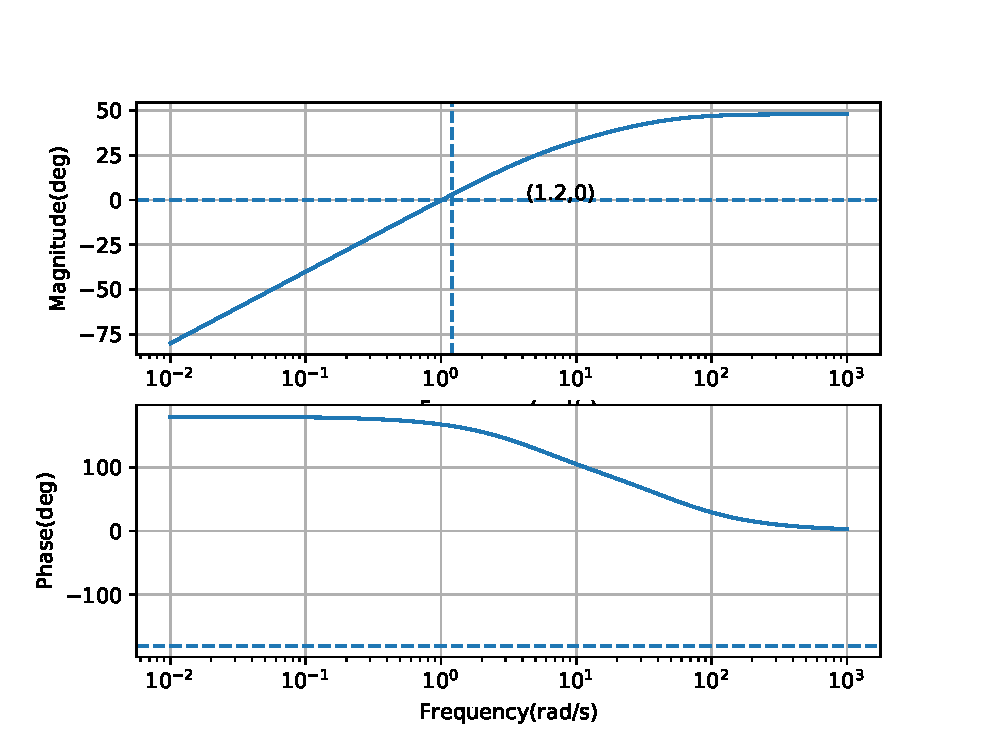
\includegraphics[width=\columnwidth]{./figs/es17btech11002/es17btech11002.eps}
\caption{}
\label{fig:es17btech11002_fig8}
\end{figure}
%
\item Find the frequency for some arbitrary R, C values given in Table \ref{table:es17btech11002_Input_Table}.\\
\begin{table}[!ht]
\centering
%%%%%%%%%%%%%%%%%%%%%%%%%%%%%%%%%%%%%%%%%%%%%%%%%%%%%%%%%%%%%%%%%%%%%%
%%                                                                  %%
%%  This is the header of a LaTeX2e file exported from Gnumeric.    %%
%%                                                                  %%
%%  This file can be compiled as it stands or included in another   %%
%%  LaTeX document. The table is based on the longtable package so  %%
%%  the longtable options (headers, footers...) can be set in the   %%
%%  preamble section below (see PRAMBLE).                           %%
%%                                                                  %%
%%  To include the file in another, the following two lines must be %%
%%  in the including file:                                          %%
%%        \def\inputGnumericTable{}                                 %%
%%  at the beginning of the file and:                               %%
%%        \input{name-of-this-file.tex}                             %%
%%  where the table is to be placed. Note also that the including   %%
%%  file must use the following packages for the table to be        %%
%%  rendered correctly:                                             %%
%%    \usepackage[latin1]{inputenc}                                 %%
%%    \usepackage{color}                                            %%
%%    \usepackage{array}                                            %%
%%    \usepackage{longtable}                                        %%
%%    \usepackage{calc}                                             %%
%%    \usepackage{multirow}                                         %%
%%    \usepackage{hhline}                                           %%
%%    \usepackage{ifthen}                                           %%
%%  optionally (for landscape tables embedded in another document): %%
%%    \usepackage{lscape}                                           %%
%%                                                                  %%
%%%%%%%%%%%%%%%%%%%%%%%%%%%%%%%%%%%%%%%%%%%%%%%%%%%%%%%%%%%%%%%%%%%%%%



%%  This section checks if we are begin input into another file or  %%
%%  the file will be compiled alone. First use a macro taken from   %%
%%  the TeXbook ex 7.7 (suggestion of Han-Wen Nienhuys).            %%
\def\ifundefined#1{\expandafter\ifx\csname#1\endcsname\relax}


%%  Check for the \def token for inputed files. If it is not        %%
%%  defined, the file will be processed as a standalone and the     %%
%%  preamble will be used.                                          %%
\ifundefined{inputGnumericTable}

%%  We must be able to close or not the document at the end.        %%
	\def\gnumericTableEnd{\end{document}}


%%%%%%%%%%%%%%%%%%%%%%%%%%%%%%%%%%%%%%%%%%%%%%%%%%%%%%%%%%%%%%%%%%%%%%
%%                                                                  %%
%%  This is the PREAMBLE. Change these values to get the right      %%
%%  paper size and other niceties.                                  %%
%%                                                                  %%
%%%%%%%%%%%%%%%%%%%%%%%%%%%%%%%%%%%%%%%%%%%%%%%%%%%%%%%%%%%%%%%%%%%%%%

	\documentclass[12pt%
			  %,landscape%
                    ]{report}
       \usepackage[latin1]{inputenc}
       \usepackage{fullpage}
       \usepackage{color}
       \usepackage{array}
       \usepackage{longtable}
       \usepackage{calc}
       \usepackage{multirow}
       \usepackage{hhline}
       \usepackage{ifthen}

	\begin{document}


%%  End of the preamble for the standalone. The next section is for %%
%%  documents which are included into other LaTeX2e files.          %%
\else

%%  We are not a stand alone document. For a regular table, we will %%
%%  have no preamble and only define the closing to mean nothing.   %%
    \def\gnumericTableEnd{}

%%  If we want landscape mode in an embedded document, comment out  %%
%%  the line above and uncomment the two below. The table will      %%
%%  begin on a new page and run in landscape mode.                  %%
%       \def\gnumericTableEnd{\end{landscape}}
%       \begin{landscape}


%%  End of the else clause for this file being \input.              %%
\fi

%%%%%%%%%%%%%%%%%%%%%%%%%%%%%%%%%%%%%%%%%%%%%%%%%%%%%%%%%%%%%%%%%%%%%%
%%                                                                  %%
%%  The rest is the gnumeric table, except for the closing          %%
%%  statement. Changes below will alter the table's appearance.     %%
%%                                                                  %%
%%%%%%%%%%%%%%%%%%%%%%%%%%%%%%%%%%%%%%%%%%%%%%%%%%%%%%%%%%%%%%%%%%%%%%

\providecommand{\gnumericmathit}[1]{#1} 
%%  Uncomment the next line if you would like your numbers to be in %%
%%  italics if they are italizised in the gnumeric table.           %%
%\renewcommand{\gnumericmathit}[1]{\mathit{#1}}
\providecommand{\gnumericPB}[1]%
{\let\gnumericTemp=\\#1\let\\=\gnumericTemp\hspace{0pt}}
 \ifundefined{gnumericTableWidthDefined}
        \newlength{\gnumericTableWidth}
        \newlength{\gnumericTableWidthComplete}
        \newlength{\gnumericMultiRowLength}
        \global\def\gnumericTableWidthDefined{}
 \fi
%% The following setting protects this code from babel shorthands.  %%
 \ifthenelse{\isundefined{\languageshorthands}}{}{\languageshorthands{english}}
%%  The default table format retains the relative column widths of  %%
%%  gnumeric. They can easily be changed to c, r or l. In that case %%
%%  you may want to comment out the next line and uncomment the one %%
%%  thereafter                                                      %%
\providecommand\gnumbox{\makebox[0pt]}
%%\providecommand\gnumbox[1][]{\makebox}

%% to adjust positions in multirow situations                       %%
\setlength{\bigstrutjot}{\jot}
\setlength{\extrarowheight}{\doublerulesep}

%%  The \setlongtables command keeps column widths the same across  %%
%%  pages. Simply comment out next line for varying column widths.  %%
\setlongtables

\setlength\gnumericTableWidth{%
	53pt+%
	93pt+%
0pt}
\def\gumericNumCols{2}
\setlength\gnumericTableWidthComplete{\gnumericTableWidth+%
         \tabcolsep*\gumericNumCols*2+\arrayrulewidth*\gumericNumCols}
\ifthenelse{\lengthtest{\gnumericTableWidthComplete > \linewidth}}%
         {\def\gnumericScale{\ratio{\linewidth-%
                        \tabcolsep*\gumericNumCols*2-%
                        \arrayrulewidth*\gumericNumCols}%
{\gnumericTableWidth}}}%
{\def\gnumericScale{1}}

%%%%%%%%%%%%%%%%%%%%%%%%%%%%%%%%%%%%%%%%%%%%%%%%%%%%%%%%%%%%%%%%%%%%%%
%%                                                                  %%
%% The following are the widths of the various columns. We are      %%
%% defining them here because then they are easier to change.       %%
%% Depending on the cell formats we may use them more than once.    %%
%%                                                                  %%
%%%%%%%%%%%%%%%%%%%%%%%%%%%%%%%%%%%%%%%%%%%%%%%%%%%%%%%%%%%%%%%%%%%%%%

\ifthenelse{\isundefined{\gnumericColA}}{\newlength{\gnumericColA}}{}\settowidth{\gnumericColA}{\begin{tabular}{@{}p{53pt*\gnumericScale}@{}}x\end{tabular}}
\ifthenelse{\isundefined{\gnumericColB}}{\newlength{\gnumericColB}}{}\settowidth{\gnumericColB}{\begin{tabular}{@{}p{93pt*\gnumericScale}@{}}x\end{tabular}}

\begin{tabular}[c]{%
	b{\gnumericColA}%
	b{\gnumericColB}%
	}

%%%%%%%%%%%%%%%%%%%%%%%%%%%%%%%%%%%%%%%%%%%%%%%%%%%%%%%%%%%%%%%%%%%%%%
%%  The longtable options. (Caption, headers... see Goosens, p.124) %%
%	\caption{The Table Caption.}             \\	%
% \hline	% Across the top of the table.
%%  The rest of these options are table rows which are placed on    %%
%%  the first, last or every page. Use \multicolumn if you want.    %%

%%  Header for the first page.                                      %%
%	\multicolumn{2}{c}{The First Header} \\ \hline 
%	\multicolumn{1}{c}{colTag}	%Column 1
%	&\multicolumn{1}{c}{colTag}	\\ \hline %Last column
%	\endfirsthead

%%  The running header definition.                                  %%
%	\hline
%	\multicolumn{2}{l}{\ldots\small\slshape continued} \\ \hline
%	\multicolumn{1}{c}{colTag}	%Column 1
%	&\multicolumn{1}{c}{colTag}	\\ \hline %Last column
%	\endhead

%%  The running footer definition.                                  %%
%	\hline
%	\multicolumn{2}{r}{\small\slshape continued\ldots} \\
%	\endfoot

%%  The ending footer definition.                                   %%
%	\multicolumn{2}{c}{That's all folks} \\ \hline 
%	\endlastfoot
%%%%%%%%%%%%%%%%%%%%%%%%%%%%%%%%%%%%%%%%%%%%%%%%%%%%%%%%%%%%%%%%%%%%%%

\hhline{|-|-}
	 \multicolumn{1}{|p{\gnumericColA}|}%
	{\gnumericPB{\centering}\gnumbox{\textbf{Parameter}}}
	&\multicolumn{1}{p{\gnumericColB}|}%
	{\gnumericPB{\centering}\gnumbox{\textbf{Value}}}
\\
\hhline{|--|}
	 \multicolumn{1}{|p{\gnumericColA}|}%
	{\gnumericPB{\centering}\gnumbox{$R$}}
	&\multicolumn{1}{p{\gnumericColB}|}%
	{$250 \Omega$}
\\
\hhline{|--|}
	 \multicolumn{1}{|p{\gnumericColA}|}%
	{\gnumericPB{\centering}\gnumbox{$C$}}
	&\multicolumn{1}{p{\gnumericColB}|}%
	{$1mF$}
\\
\hhline{|-|-|}
	 \multicolumn{1}{|p{\gnumericColA}|}%
	{\gnumericPB{\centering}\gnumbox{$R_{2}$}}
	&\multicolumn{1}{p{\gnumericColB}|}%
	{$2030\Omega $}
\\
\hhline{|--|}
	 \multicolumn{1}{|p{\gnumericColA}|}%
	{\gnumericPB{\centering}\gnumbox{$R_{1}$}}
	&\multicolumn{1}{p{\gnumericColB}|}%
	{$1000\Omega $}	
\\
\hhline{|-|-|}
\end{tabular}

\ifthenelse{\isundefined{\languageshorthands}}{}{\languageshorthands{\languagename}}
\gnumericTableEnd

\caption{}
\label{table:es17btech11002_Input_Table}
\end{table}
\\
\solution 
%
\textbf{Frequency:} From equation \eqref{eq:es17btech11002_freq}
\begin{align}
\omega = \frac{1}{RC} = 10000 rad/sec
\end{align}
\begin{align}
f = \frac{\omega }{2\pi} = 1.57 kHz
\end{align}
\item Verify the frequency using spice simulation.\\
\solution The following readme file provides necessary instructions to simulate the circuit in spice.
\begin{lstlisting}
codes/es17btech11002/spice/README
\end{lstlisting}
The following netlist simulates the given circuit.
\begin{lstlisting}
codes/es17btech11002/spice/es17btech11002.net
\end{lstlisting}
The following code plots the output from the oscillator spice simulation which is shown in Fig. \ref{fig:es17btech11002_spice}.
\begin{lstlisting}
codes/es17btech11002/spice/es17btech11002_spice.py
\end{lstlisting}
\renewcommand{\thefigure}{\theenumi.\arabic{figure}}
%
\begin{figure}[!ht]
\centering
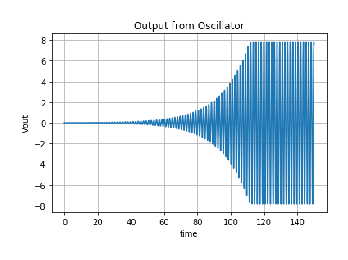
\includegraphics[width=\columnwidth]{./figs/es17btech11002/es17btech11002_spice.eps}
\caption{}
\label{fig:es17btech11002_spice}
\end{figure}
%
The following code plots a part of the spice output from which we can observe a clear sinusoidal output shown in Fig. \ref{fig:es17btech11002_spice2}.
\begin{lstlisting}
codes/es17btech11002/spice/es17btech11002_spice2.py
\end{lstlisting}
\begin{figure}[!ht]
\centering
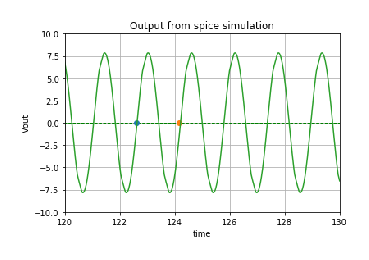
\includegraphics[width=\columnwidth]{./figs/es17btech11002/es17btech11002_spice2.eps}
\caption{}
\label{fig:es17btech11002_spice2}
\end{figure}
\renewcommand{\thefigure}{\theenumi}
\textbf{Amplitude:}From Fig. \ref{fig:es17btech11002_spice2} V(peak-peak) is 
\begin{align}
V_{p-p} &= 0.47-(-0.47) = 0.94V
\end{align}
\begin{align}
V_{max} &= \frac{V_{p-p}}{2} = 0.47.
\end{align}
\textbf{Frequency:} time period is calculated by any two end points of one cycle,
\begin{align}
T&=0.0313164 - \brak{0.03060} = 0.7164 ms
\end{align}
\begin{align}
f = \frac{1}{T} = 1.39 kHz
\end{align}
Hence,the frequency is verified through the spice simulation.
\end{enumerate}

For the feedback transresistance amplifier in Fig. , use small-signal analysis to find the open-loop gain G, the feedback H, and the closed loop gain $G_m$. Neglect $r_o$ of each of the transistors and assume $R_C << \beta_2R_E$ and $R_E << R_F$, and that the feedback causes the signal voltage at the input node to be nearly zero. Evaluate $/frac{V_o}{I_s}$ for the following component values: $\beta_1 = \beta_2 = 100$ , $R_C = R_E = 10 k\ohm$ and $R_F = 100 k\ohm$.

\begin{enumerate}[label=\arabic*.,ref=\theenumi]
%\begin{enumerate}[label=\thesection.\arabic*.,ref=\thesection.\theenumi]
\numberwithin{equation}{enumi}

\item Draw the small-signal equivalent of the circuit in Fig.\ref{fig:ee18btech11045_fb_question}.

\begin{figure}[h!]
	\begin{center}
		\resizebox{\columnwidth}{!}{\begin{circuitikz}[american]
\draw (0,0) node[npn](npn1){Q1}
(npn1.B) -- (-2,0) (-2,-2) to[I , l = $I_{in}$] (-2,0) (-2,-2) node[ground]{}
(npn1.E) -- (0,-1) node[ground]{}
(npn1.C) to[R, l_=$R_{C}$] (0,4) to[short,-o]++(0,0.5) node[right]{$V_{cc}$};

\draw (3,1) node[npn](npn2){Q2}
(npn2.B) -- (0,1) 
(npn2.C) -- (3,4) to[short,-o]++(0,0.5) node[right]{$V_{cc}$}
(npn2.E) to[R, l_ = $R_{E}$] (3,-3) to[short,-o]++(0,-0.5) node[left]{$-V_{ee}$}

(3,0) to[short,-o]++(2,0) node[right]{$V_{out}$}
(4,0) -- (4,-4) to[R, l=$R_{F}$] (-1,-4) -- (-1,0)

;\end{circuitikz}}
	\end{center}
	\caption{}
	\label{fig:ee18btech11045_fb_question}
\end{figure}

\solution

\begin{figure}[h!]
	\begin{center}
		\resizebox{\columnwidth}{!}{\begin{circuitikz}[american]
 \draw (0,0) to[R, l_ = $R_{C}$] (0,3) -- (-1,3)
 (0.5,3)node[above]{$Y$}
 (-1,3)to[I,l_ = $g_{m_1}v_{\pi1}$] (-1,0) -- (0,0)
 
 (-1,0) -- (-3,0) node[ground]{} -- (-4,0) node[left]{$-$}

 (-4,0) to[R, l = $r_{\pi1}$] (-4,3)
 
 (-6,0) node[ground]{} to[I, l = $I_{in}$] (-6,3) -- (-4,3) node[right]{$+$}
 
 (0,3) -- (1.5,3) node[right]{$+$}
 %Add v2 here
 (1.5,3) to[R, l = $r_{\pi2}$] (1.5,0)
 
 (1.5,0) node[left]{$-$} -- (5,0)
 (6,3) node[ground]{} -- (5,3) to[I, l_= $g_{m_2}v_{\pi2}$] (5,0)

(3,0) to[R, l = $R_{E}$] (3,-3) node[ground]{}

(3,-0.5) to[short,-o]++(3,0) node[right]{$V_{out}$}

(4,-0.5)node[above]{$Z$} -- (4,-5) to[R, l=$R_F$] (-5,-5) 
(-5,3)node[above]{$X$} to[short, i_ = $I_F$] (-5,-5) 
;\end{circuitikz}}
	\end{center}
	\caption{}
	\label{fig:ee18btech11045_fb_smallsignalmodel}
\end{figure}

The equivalent circuit is Fig.\ref{fig:ee18btech11045_fb_smallsignalmodel}

\item Find the expression for the open loop Gain(G) of the system.

\solution

The given system is a cascaded system of $Q_1$ and $Q_2$.
The signal flow graph is illustrated in Fig. \ref{fig:ee18btech11045_fb_signalflow}

\begin{figure}[h!]
	\begin{center}
		\resizebox{\columnwidth}{!}{\begin{tikzpicture}

\draw (0,0)node[left]{$I_{in}$} to[short] (2,0)node[above]{X}
(2,0) to[short, *-*, i_ = $G_1$] (4,0) node[above]{Y}
(4,0) to[short, *-*, i_ = $G_2$] (6,0) node[above]{Z}
(6,0) to[short] (8,0)node[right]{$V_{out}$}
(6,0) -- (6,-2) to[short, i = $H$] (2,-2) -- (2,0)

;\end{tikzpicture}
}
	\end{center}
	\caption{}
	\label{fig:ee18btech11045_fb_signalflow}
\end{figure}

So, if the gain of $Q_1$ and $Q_2$ are $G_1$ and $G_2$ respectively, the open-loop gain ($G$) is given by:
\begin{align}
    G = G_1G_2
    \label{eq:ee18btech11045_fb_Gainformula}
\end{align}

$Q_1$ is in CE(Common-emitter) stage. The input signal is $I_{in}$.
From fig. \ref{fig:ee18btech11045_fb_smallsignalmodel},
\begin{align}
    I_X = I_{in}
\end{align}
\begin{align}
    \beta = \frac{I_c}{I_b}
\end{align}
Applying Kirchoff's Law in the loop connecting Y to ground,
\begin{align}
    \implies V_Y = \beta I_{in} R_C
\end{align}
\begin{align}   
    G_1 = \frac{V_{out}}{I_{in}} = \frac{V_{Y}}{I_{X}}
    \\
    =\beta R_c
\end{align}

$Q_2$ is in emitter follower topology.
\begin{align}
    V_{\pi 2}  = V_Y - V_Z
\end{align}
Applying Kirchoff's Law,
\begin{align}
    \frac{V_Y - V_Z}{r_{\pi}} + g_{m2}\brak{V_Y-V_Z} = \frac{V_Z}{R_E}
\end{align}
\begin{align}
    \implies \frac{V_Z}{V_Y} = \frac{R_E}{\frac{1}{g_{m2}} + R_E}
\end{align}
\begin{align}
    \implies G_2 = \frac{R_E}{\frac{1}{g_{m2}} + R_E}
\end{align}

From \eqref{eq:ee18btech11045_fb_Gainformula}, the open loop gain ($G$):
\begin{align}
    G = \brak{\beta_1 R_c} \brak{\frac{R_E}{\frac{1}{g_{m2}} + R_E}}
    \label{eq:ee18btech11045_fb_Gain}
\end{align}

\item Find the feedback factor(H) of the given circuit.

\solution

From Fig.\ref{fig:ee18btech11045_fb_smallsignalmodel}, the feedback circuit consists of only a resistor $R_F$:
\begin{align}
    \therefore H = \frac{I_F}{V_{out}} = \frac{1}{R_F}
    \label{eq:ee18btech11045_fb_feedbackfactor}
\end{align}

\item Find the closed loop gain of the system.

\solution 

The closed loop gain of a system is given by:
\begin{align}
    G_L = \frac{G}{1+GH}
\end{align}

From \eqref{eq:ee18btech11045_fb_Gain} and \eqref{eq:ee18btech11045_fb_feedbackfactor}. The closed loop gain of the circuit is given by:
\begin{align}
    G_L = \frac{\brak{\beta_1 R_c} \brak{\frac{R_E}{\frac{1}{g_{m2}} + R_E}}}{1 + \frac{\brak{\beta_1 R_c} \brak{\frac{R_E}{\frac{1}{g_{m2}} + R_E}}}{R_F}}
    \\
    = \frac{R_FR_CR_E\beta}{\beta R_C R_E + R_F\brak{\frac{1}{g_{m2}}+R_E}}
    \label{eq:ee18btech11045_fb_clgain}
\end{align}


\item Find G,H and $G_L$ for the given problem. Parameters are summarised in table \ref{table:ee18btech11045_table1}.
%
\begin{table}[!ht]
\centering
\def\ifundefined#1{\expandafter\ifx\csname#1\endcsname\relax}

\ifundefined{inputGnumericTable}

	\def\gnumericTableEnd{\end{document}}


%%%%%%%%%%%%%%%%%%%%%%%%%%%%%%%%%%%%%%%%%%%%%%%%%%%%%%%%%%%%%%%%%%%%%%
%%                                                                  %%
%%  This is the PREAMBLE. Change these values to get the right      %%
%%  paper size and other niceties.                                  %%
%%                                                                  %%
%%%%%%%%%%%%%%%%%%%%%%%%%%%%%%%%%%%%%%%%%%%%%%%%%%%%%%%%%%%%%%%%%%%%%%

	\documentclass[12pt%
			  %,landscape%
                    ]{report}
       \usepackage[latin1]{inputenc}
       \usepackage{fullpage}
       \usepackage{color}
       \usepackage{array}
       \usepackage{longtable}
       \usepackage{calc}
       \usepackage{multirow}
       \usepackage{hhline}
       \usepackage{ifthen}
%%  End of the preamble for the standalone. The next section is for %%
%%  documents which are included into other LaTeX2e files.          %%
\else

%%  We are not a stand alone document. For a regular table, we will %%
%%  have no preamble and only define the closing to mean nothing.   %%
    \def\gnumericTableEnd{}

%%  If we want landscape mode in an embedded document, comment out  %%
%%  the line above and uncomment the two below. The table will      %%
%%  begin on a new page and run in landscape mode.                  %%
%       \def\gnumericTableEnd{\end{landscape}}
%       \begin{landscape}


%%  End of the else clause for this file being \input.              %%
\fi

%%%%%%%%%%%%%%%%%%%%%%%%%%%%%%%%%%%%%%%%%%%%%%%%%%%%%%%%%%%%%%%%%%%%%%
%%                                                                  %%
%%  The rest is the gnumeric table, except for the closing          %%
%%  statement. Changes below will alter the table's appearance.     %%
%%                                                                  %%
%%%%%%%%%%%%%%%%%%%%%%%%%%%%%%%%%%%%%%%%%%%%%%%%%%%%%%%%%%%%%%%%%%%%%%

\providecommand{\gnumericmathit}[1]{#1} 
%%  Uncomment the next line if you would like your numbers to be in %%
%%  italics if they are italizised in the gnumeric table.           %%
%\renewcommand{\gnumericmathit}[1]{\mathit{#1}}
\providecommand{\gnumericPB}[1]%
{\let\gnumericTemp=\\#1\let\\=\gnumericTemp\hspace{0pt}}
 \ifundefined{gnumericTableWidthDefined}
        \newlength{\gnumericTableWidth}
        \newlength{\gnumericTableWidthComplete}
        \newlength{\gnumericMultiRowLength}
        \global\def\gnumericTableWidthDefined{}
 \fi
%% The following setting protects this code from babel shorthands.  %%
 \ifthenelse{\isundefined{\languageshorthands}}{}{\languageshorthands{english}}
%%  The default table format retains the relative column widths of  %%
%%  gnumeric. They can easily be changed to c, r or l. In that case %%
%%  you may want to comment out the next line and uncomment the one %%
%%  thereafter                                                      %%
\providecommand\gnumbox{\makebox[0pt]}
%%\providecommand\gnumbox[1][]{\makebox}

%% to adjust positions in multirow situations                       %%
\setlength{\bigstrutjot}{\jot}
\setlength{\extrarowheight}{\doublerulesep}

%%  The \setlongtables command keeps column widths the same across  %%
%%  pages. Simply comment out next line for varying column widths.  %%
\setlongtables

\setlength\gnumericTableWidth{%
	60pt+%
	100pt+%
0pt}
\def\gumericNumCols{2}
\setlength\gnumericTableWidthComplete{\gnumericTableWidth+%
         \tabcolsep*\gumericNumCols*2+\arrayrulewidth*\gumericNumCols}
\ifthenelse{\lengthtest{\gnumericTableWidthComplete > \linewidth}}%
         {\def\gnumericScale{\ratio{\linewidth-%
                        \tabcolsep*\gumericNumCols*2-%
                        \arrayrulewidth*\gumericNumCols}%
{\gnumericTableWidth}}}%
{\def\gnumericScale{1}}

%%%%%%%%%%%%%%%%%%%%%%%%%%%%%%%%%%%%%%%%%%%%%%%%%%%%%%%%%%%%%%%%%%%%%%
%%                                                                  %%
%% The following are the widths of the various columns. We are      %%
%% defining them here because then they are easier to change.       %%
%% Depending on the cell formats we may use them more than once.    %%
%%                                                                  %%
%%%%%%%%%%%%%%%%%%%%%%%%%%%%%%%%%%%%%%%%%%%%%%%%%%%%%%%%%%%%%%%%%%%%%%

\ifthenelse{\isundefined{\gnumericColA}}{\newlength{\gnumericColA}}{}\settowidth{\gnumericColA}{\begin{tabular}{@{}p{60pt*\gnumericScale}@{}}x\end{tabular}}
\ifthenelse{\isundefined{\gnumericColB}}{\newlength{\gnumericColB}}{}\settowidth{\gnumericColB}{\begin{tabular}{@{}p{100pt*\gnumericScale}@{}}x\end{tabular}}
\begin{tabular}[c]{%
	b{\gnumericColA}%
	b{\gnumericColB}%%
	}



\hhline{|-|-}
	 \multicolumn{1}{|p{\gnumericColA}|}%
	{\gnumericPB{\centering}\textbf{Parameters}}
	&\multicolumn{1}{p{\gnumericColB}|}%
	{\gnumericPB{\centering}\textbf{Value}}

\\
\hhline{|--|}
	 \multicolumn{1}{|p{\gnumericColA}|}%
	{\gnumericPB{\centering}$V_{cc}$}
	&\multicolumn{1}{p{\gnumericColB}|}%
	{\gnumericPB{\centering}$5 V$}
	

\\
\hhline{|--|}
	 \multicolumn{1}{|p{\gnumericColA}|}%
	{\gnumericPB{\centering}$\beta_1$}
	&\multicolumn{1}{p{\gnumericColB}|}%
	{\gnumericPB{\centering}$100$}

\\
\hhline{|--|}
	 \multicolumn{1}{|p{\gnumericColA}|}%
	{\gnumericPB{\centering}$\beta_2$}
	&\multicolumn{1}{p{\gnumericColB}|}%
	{\gnumericPB{\centering}$100$}

\\
\hhline{|--|}
	 \multicolumn{1}{|p{\gnumericColA}|}%
	{\gnumericPB{\centering}$R_{C}$}
	&\multicolumn{1}{p{\gnumericColB}|}%
	{\gnumericPB{\centering}$10K\ohm$}

\\
\hhline{|--|}
	 \multicolumn{1}{|p{\gnumericColA}|}%
	{\gnumericPB{\centering}$R_{E}$}
	&\multicolumn{1}{p{\gnumericColB}|}%
	{\gnumericPB{\centering}$10K\ohm$}
	
\\
\hhline{|--|}
	 \multicolumn{1}{|p{\gnumericColA}|}%
	{\gnumericPB{\centering}$R_{F}$}
	&\multicolumn{1}{p{\gnumericColB}|}%
	{\gnumericPB{\centering}$100K\ohm$}

\\
\hhline{|-|-|}
\end{tabular}

\ifthenelse{\isundefined{\languageshorthands}}{}{\languageshorthands{\languagename}}
\gnumericTableEnd
\caption{}
\label{table:ee18btech11045_table1}
\end{table}

\solution

To calculate the bias values of Q1, Q2. Remove the input and output, the resultant circuit is shown in fig.\ref{fig:biascalc}

\begin{figure}[!ht]
	\begin{center}
			\resizebox{\columnwidth}{!}{\begin{circuitikz}[american]
\draw (0,0) node[npn](npn1){Q1}
(-1,0) to[short, i = $I_{b1}$] (npn1.B)
(npn1.E) -- (0,-1) node[ground]{}
(0,4) to[R, l_=$R_{C}$, i_ = $\beta I_{b1}$ ] (npn1.C)
(0,4) to[short,-o]++(0,0.5) node[right]{$V_{cc}$};

\draw (3,1) node[npn](npn2){Q2}
(0,1) to[short, i = $I_{b2}$] (npn2.B)
(npn2.C) -- (3,4) to[short,-o]++(0,0.5) node[right]{$V_{cc}$}
(npn2.E) to[short, i_ = $(\beta+1)I_{b2}$ ] (3,0) to[R, l_ = $R_{E}$, i_ = $(\beta+1)I_{b2} + I_{b_1}$] (3,-3) to[short,-o]++(0,-0.5) node[left]{$-V_{ee}$}

(3,0) -- (4,0) -- (4,-4) to[R, l=$R_{F}$] (-1,-4) -- (-1,0)

;\end{circuitikz}}
	\end{center}
\caption{}
\label{fig:biascalc}
\end{figure}

Applying KVL to the circuit, we get:
\begin{align}
    0.7  + I_{b1}R_F + \brak{I_{b1} - (\beta+1)I_{b2}}R_E = -V_{ee}
\end{align}
\begin{align}
    0.7 + I_{b1}R_F + 0.7 + \brak{\beta I_{b1} + I_{b2}}R_C = V_{cc}
\end{align}

Solving the above equations, we get:
\begin{align}
    I_{b1} = \frac{\frac{V_{cc} - 1.4}{R_C} - \frac{V_{ee} +0.7}{R_E(\beta+1)}}{\frac{R_F + \beta R_C}{R_C} + \frac{R_E + R_F}{R_E(\beta + 1)}}
    \\
    = 3.22 * 10^{-6}
\end{align}
\begin{align}
    I_{b2} = \frac{\frac{V_{cc} - 1.4}{\beta R_C + R_F} + \frac{V_{ee}+0.7}{R_E+R_F}}{\frac{R_C}{R_F+\beta R_C} + \frac{R_E(\beta+1)}{R_E+R_F}}
\end{align}

we know, 
\begin{align}
    g_m = \frac{I_{c}}{V_T}
\end{align}
where, $V_T$ = 26mV, and
\begin{align}
    r_{\pi} = \frac{\beta}{g_m}
\end{align}

\begin{align}
    \therefore g_{m1} &= \frac{\beta I_{b1}}{V_T}
    \\
    &= 0.0123
\end{align}
\begin{align}
    r_{\pi 1} &= \frac{\beta}{g_{m1}}
    \\
    &= 8130 \ohm
\end{align}
\begin{align}    
    \therefore g_{m2} &= \frac{\beta I_{b2}}{V_T}
    \\
    &= 0.023
\end{align}
\begin{align}
    r_{\pi 2} &= \frac{\beta}{g_{m2}}
    \\
    &= 4347.8 \ohm
\end{align}

From \eqref{eq:ee18btech11045_fb_Gain}, the open loop gain (G):
\begin{align}
    G &= \brak{100*(10K)}\brak{\frac{10^{4}}{10^{4} + \frac{1}{0.023}}} \ohm
    \\
    &= \brak{10^{6}}\brak{0.995}
    \\
    &= 995670 \ohm
\end{align}

From \eqref{eq:ee18btech11045_fb_feedbackfactor}, the feedback (H):
\begin{align}
    H = \frac{1}{100K} \ohm^{-1}
    \implies H = 10^{-5} \ohm^{-1}
\end{align}

From \eqref{eq:ee18btech11045_fb_clgain}, the closed loop gain ($G_L$):
\begin{align}
    G_L &= \frac{995670}{1 + (995670)(10^{-5})} \ohm
    \\
    &= 99006.52 \ohm
    \label{ee18btech11045_closedloopgaincl}
\end{align}

\item Verify the result using spice simulation.

\solution

The following netlist simulates the closed loop gain for a sinusoidal signal of amplitude $10^{-6}$
\begin{lstlisting}
codes/ee18btech11045/spice/ee18btech11045_clresult.net
\end{lstlisting}

The output is plotted using the folowing code.
\begin{lstlisting}
codes/ee18btech11045/spice/ee18btech11045_clresult.py
\end{lstlisting}

The output is plotted in fig. \ref{fig:ee18btech11045_fb_clresult}. The output amplitude is shown to be 0.1 .
\begin{align}
    \therefore \frac{V_{out}}{I_{in}} \approx 10^{5}
\end{align}
This proves the value calculated in \eqref{ee18btech11045_closedloopgaincl}.

\begin{figure}[h!]
	\begin{center}
		\resizebox{\columnwidth/1}{!}{\input{./figs/ee18btech11045/ee18btech11045_clresult.eps}}
	\end{center}
	\caption{}
	\label{fig:ee18btech11045_fb_clresult}
\end{figure}

\item Represent the circuit using a Feedback Block diagram.

\solution

\begin{figure}[!ht]
	\begin{center}
			\resizebox{\columnwidth}{!}{\begin{circuitikz}[american]
\usetikzlibrary{positioning, fit, calc}
\draw (0,0) to[I = $I_{in}$, *-*] (0,2) to[short, *-*] (2,2)node[above]{$+$} to[R=$R_{in}$,*-*] (2,0)node[below]{$-$}
(2-0.2,1) node[left]{$V_{in}$}
(2,2) to[short, *-*] (5,2) {}
(7,1)node[draw,minimum width=4cm,minimum height=4cm] (load) {Gain Amplifier}{}
(7,-4)node[draw,minimum width=4cm,minimum height=4cm] (load) {Feedback Network}{}
(0,0) to[short, *-*] (5,0)
(14,2) to[R = $R_{out}$, *-*] (9,2)
(14,2) node[right]{$+$}
(14,1) node[]{$V_{out}$}
(14,0) node[right]{$-$}
(14,0) to[short, *-*] (9,0)
(3,0) to[short, *-*] (3,-5) to[short, *-*] (5,-5){}
(4,2) to[short, *-*, i = $I_F$] (4,-3)
(4,-3) to[short, *-*] (5,-3){}
(10,2) to[short, *-*] (10,-3) to[short, *-*] (9,-3){}
(9,-5) to[short, *-*] (11,-5) to[short, *-*] (11,0){}
;\end{circuitikz}}
	\end{center}
\caption{Shunt-Shunt Feedback}
\label{fig:Block_Diagram}
\end{figure}

\item Calculate the input resistance of the open loop and closed loop system and compare.

\solution

For the cascaded system of $Q1$ and $Q2$, the input resistance of the system $R_{in}$,
\begin{align}
    R_{in} = R_{in_{Q1}}   
\end{align}

To calculate the input resistance of the system, shot the independent sources  and find the ratio $\frac{V_in}{I_in}$. As, $Q1$ is in common-emitter stage, from the fig. \ref{fig:ee18btech11045_fb_smallsignalmodel},
\begin{align}
    R_in &= r_{\pi1}
    \\
    &= 8130 \ohm
\end{align}

After feedback is applied, to calculate input resistance, consider an input source $V_{in}$ is connected to the input,
\begin{align}
    V_{out} &= I_{in}G
    &= \frac{V_{in}}{R_{in}}G
\end{align}
But as feedback is applied,
\begin{align}
    V_{in} &= V_{out} H
    &= \frac{V_{in}}{R_{in}}GH
\end{align}
Applying KVL for input loop in fig. \ref{fig:Block_Diagram},
\begin{align}
    \brak{I_{in} - \frac{V_{in}}{R_{in}}GK}R_{in} = V_{in}
\end{align}
\begin{align}
    \implies R_{in_{cl}} = \frac{V_{in}}{I_{in}} = \frac{R_in}{1+GH}
\end{align}
where, $R_in$ is the input resistance of open loop.Therefore, $R_{in}$ after feedback:
\begin{align}
    R_{in} &= \frac{r_{pi1}}{1 + GH}
    \\
    &= \frac{8130}{10.95} = 742 \ohm
\end{align}

The input should act as an ideal current source, so as the input resistance is decreased, the feedback gives more favourable value of $R_{in}$.

\item Calculate the output resistance of the open loop and closed loop system and compare.

\solution

Similar to the input resistance, the output resistance of the cascaded system is the output resistance of $Q2$. As $Q2$ is in emitter follower configuration, from the fig. \ref{fig:ee18btech11045_fb_smallsignalmodel},

\begin{align}
    R_{out} &= \frac{1}{g_{m2}}
    \\
    &= \frac{1}{0.023} = 43.37 \ohm
\end{align}

To calculate output resistance after feedback is applied, consider a voltage source $V_X$ applied at $V_{out}$ with output current $I_X$ :
\begin{align}
    V_{in} = HV_{X}
\end{align}
\begin{align}
    \implies V_{out} = GHV_{X}
\end{align}
Applying KVL at ouput loop,
\begin{align}
    \frac{GHV_X+V_X}{R_{out}} = I_X
\end{align}
The closed loop output impedance,
\begin{align}
    R_{out_{cl}} &= \frac{V_X}{I_X}
    \\
    &= \frac{R_{out}}{1 + GH}
\end{align}
The output resistance after feedback:
\begin{align}
    R_{out} = \frac{43.37}{10.95} = 3.96 \ohm
\end{align}

The ouput should act as an ideal voltage source, i.e the output resistance should be as low as possible. As feedback reduces the values of $R_{out}$, it causes the output resistances to be more favourable.

\end{enumerate}
\end{enumerate}

\section{Stability in Frequency Domain}

\subsection{Nyquist Criterion}
\begin{enumerate}[label=\thesubsection.\arabic*.,ref=\thesubsection.\theenumi]
\numberwithin{equation}{enumi}
%\begin{enumerate}[label=\thesection.\arabic*.,ref=\thesection.\theenumi]
%\numberwithin{equation}{enumi}
\item Using Nyquist criterion find the range of $K$ for which closed loop system is stable.
\begin{align}
    G(s) = \frac{K}{s(s+6)}
    \label{eq:ee18btech11028_1_1}
\\
    H(s) = \frac{1}{s+9}
    \label{eq:ee18btech11028_1_2}
\end{align}

\solution
The system flow can be described as,

\begin{figure}[!ht]
    \begin{center}
        \resizebox{\columnwidth}{!}{%\begin{figure}
\tikzstyle{block} = [draw, fill=blue!20, rectangle, 
        minimum height=1cm, minimum width=1cm]
\tikzstyle{sum} = [draw, fill=blue!20, circle, node distance=1cm]
\tikzstyle{input} = [coordinate]
\tikzstyle{output} = [coordinate]
\tikzstyle{pinstyle} = [pin edge={to-,thin,black}]
    
    % The block diagram code is probably more verbose than necessary
\begin{tikzpicture}[auto, node distance=2cm,>=latex']
    % We start by placing the blocks
    \node [input, name=input] {X(s)};
    \node [sum, right of=input] (sum) {};
    \node [block, right of=sum] (controller) {$\frac{1}{s(s+6)}$};
    \node [block, right of=controller] (system) {$K$};
        % We draw an edge between the controller and system block to 
        % calculate the coordinate u. We need it to place the measurement block. 
    \draw [->] (controller) -- node[name=u] {} (system);
    \node [output, right of=system] (output) {};
    \node [block, below of=u] (measurements) {H(s)};
    
    % Once the nodes are placed, connecting them is easy. 
    \draw [draw,->] (input) -- node {$X(s)$} (sum);
    \draw [->] (sum) -- node {} (controller);
    \draw [->] (system) -- node [name=y] {$Y(s)$}(output);
    \draw [->] (y) |- (measurements);
    \draw [->] (measurements) -| node[pos=0.99] {$-$} 
        node [near end] {} (sum);
\end{tikzpicture}
%\end{figure}
}
    \end{center}
    \caption{}  
    \label{fig:ee18btech11028_1_fig1}
\end{figure}


\begin{align}
    G_{1}(s) = \frac{1}{s(s+6)}. 
    \label{eq:ee18btech11028_1_3}
\end{align}

For Nyquist plot, 

\begin{align}
    \text{Im} \cbrak{G_{1}(\j \omega)H(\j \omega)} &= \frac{-(54 - \omega^{2})}{(\omega)(\omega^{2}+56)(\omega^{2} + 81)}
    \label{eq:ee18btech11028_1_5}
\\
    \text{Re} \cbrak{G_{1}(\j \omega)H(\j \omega)} &= \frac{-15 \omega}{(\omega)(\omega^{2}+56)(\omega^{2} + 81)}
    \label{eq:ee18btech11028_1_4}
\end{align}

From \eqref{eq:ee18btech11028_1_5} and \eqref{eq:ee18btech11028_1_4}

\begin{figure}[!h]
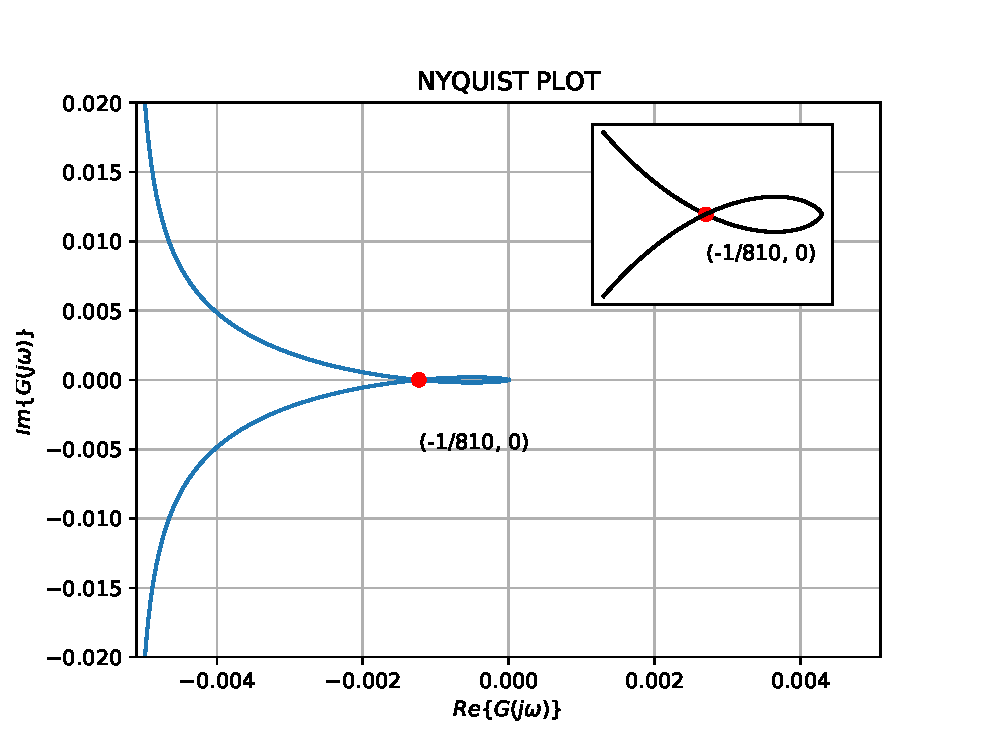
\includegraphics[width=\columnwidth]{./figs/ee18btech11028_1.eps}
    \centering
  \caption{Nyquist plot for $G_{1}(s)H(s)$}
  \label{fig:ee18btech11028_1_fig2}
\end{figure}


\textbf{Nyquist Stability Criterion:}
\begin{align}
    N = Z - P
\end{align}

where Z is \# unstable poles of closed loop transfer function, P is \# unstable poles of open loop transfer function
and N is \# clockwise encirclement of \brak{-1/K,0}.

For stable system, 
\begin{align}
    Z = 0
\end{align}

From \eqref{eq:ee18btech11028_1_2} and \eqref{eq:ee18btech11028_1_3},
\begin{align}
    P = 0
\\
    \implies N = 0
    \label{eq:ee18btech11028_1_7}
\end{align}




Since, there is a zero at origin, an infinite radius half circle will enclose the right hand side of end points of the Nyquist plot.
So for \eqref{eq:ee18btech11028_1_7},
\begin{align}
    \implies \frac{-1}{K} < \frac{-1}{810}
    \implies K < 810
\end{align}

And also,

\begin{align}
    K > 0
\\
    \implies 0 < K < 810     
\end{align}


The following python code generates  Fig. \ref{fig:ee18btech11028_1_fig2}
\begin{lstlisting}
    codes/ee18btech11028_1.py
\end{lstlisting}
%\end{enumerate}

\begin{enumerate}[label=\thesection.\arabic*.,ref=\thesection.\theenumi]
\numberwithin{equation}{enumi}
\item In a system whose signal flow graph is shown in the figure, $U_1(s)$ and $U_2(s)$ are inputs. Find the  transfer function $\frac{Y(s)}{U_1(s)}$.
%
\begin{figure}[!ht]
\begin{center}
		
		\resizebox{\columnwidth}{!}{\usetikzlibrary{decorations.markings}
\newif\iflabrev
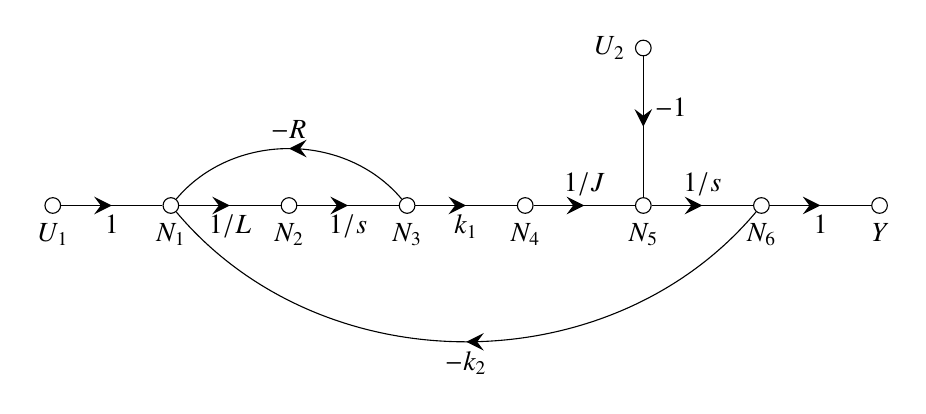
\begin{tikzpicture}
[
label revd/.is if=labrev,
amark/.style={
            decoration={             
                        markings,   
                        mark=at position {0.5} with { 
                                    \arrow[scale=2,>=stealth]{>},
                                    \iflabrev \node[above] {#1};\else \node[below] {#1};\fi
                        }
            },
            postaction={decorate}
},
terminal/.style 2 args={draw,circle,inner sep=2pt,label={#1:#2}},
]

\node[terminal={below}{$U_1$}] (a) at (0,0) {};
\node[terminal={below }{$N_1$}] (b) at (1.5cm,0) {};
\node[terminal={below}{$N_2$}] (c) at (3cm,0) {};
\node[terminal={below }{$N_3$}] (d) at (4.5cm,0) {};
\node[terminal={below }{$N_4$}] (e) at (6cm,0) {};
\node[terminal={below }{$N_5$}] (f) at (7.5cm,0) {};
\node[terminal={below }{$N_6$}] (g) at (9cm,0) {};
\node[terminal={below }{$Y$}] (h) at (10.5cm,0) {};
\node[terminal={left }{$U_2$}] (i) at (7.5cm,2cm) {};

\draw[amark=$1$] (a) to (b);
\draw[amark=$1/L$] (b) to (c);
\draw[amark=$1/s$] (c)to(d);
\draw[amark=$k_1$] (d) to (e);
\draw[amark=$1/J$,label revd] (e) to (f);
\draw[amark=$1/s$,label revd] (f) to (g);
\draw[amark=$1$] (g) to (h);
\draw[amark=$\hspace{0.7cm}-1$,label revd] (i) to (f);

\draw[amark=$-R$,label revd] (d) to[bend left=-50]  (b);
\draw[amark=$-k_2$] (g) to[bend left=50]  (b);



\end{tikzpicture}}
	\end{center}
	\label{fig:ee18btech11041}
\end{figure}
\\
\solution The desired transfer function is given by
\begin{align}
    \frac{Y(s)}{U_1(s)}\Biggr|_{U_2(s)=0}
    \label{eq:ee18btech11041_1}
\end{align}
%
The corresponding transition equations are
\begin{align}
    N_1 &= U_1-RN_3-k_2N_6
    \label{eq:ee18btech11041_2}
\\
    N_2&=\frac{N_1}{L}
    \label{eq:ee18btech11041_4}
\\
    N_3&=\frac{N_2}{s}
    \label{eq:ee18btech11041_5}
\\
    N_4&=k_1N_3
    \label{eq:ee18btech11041_6}
\\
    N_5&=\frac{N_4}{J}
    \label{eq:ee18btech11041_7}
\\
    N_6&=\frac{N_5}{s}
    \label{eq:ee18btech11041_8}
\end{align}
and the state transition matrix is
\begin{align}
    \Vec{T} = \myvec{0 & 0 & -R & 0 & 0 & -k_2\\
    \frac{1}{L} & 0 & 0 & 0 & 0 & 0\\
    0 & \frac{1}{s} & 0 & 0 & 0 & 0\\
    0 & 0 & k_1 & 0 & 0 & 0\\
    0 & 0 & 0 & \frac{1}{J} & 0 & 0\\
    0 & 0 & 0 & 0 & \frac{1}{s} & 0}
    \label{eq:ee18btech11041_9}
\end{align}    
Defining 
\begin{align}
    \Vec{U} &= {(\Vec{I}-\Vec{T})^-}^1
    \label{eq:ee18btech11041_10}
\\
     &= \myvec{1 & 0 & R & 0 & 0 & k_2\\
    \frac{-1}{L} & 1 & 0 & 0 & 0 & 0\\
    0 & \frac{-1}{s} & 1 & 0 & 0 & 0\\
    0 & 0 & -k_1 & 1 & 0 & 0\\
    0 & 0 & 0 & \frac{-1}{J} & 1 & 0\\
    0 & 0 & 0 & 0& \frac{-1}{s} & 1 }^{-1}
    \label{eq:ee18btech11041_10}
\end{align}
the gain of the system is given by 
\begin{align}
   U_{50} =  \frac{Y(s)}{U_1(s)}=\frac{k_1}{s^2LJ+sRJ+k_1k_2}
    \label{eq:ee18btech11041_12}
\end{align}
%
computed by 
\begin{lstlisting}
codes/ee18btech11041.py
\end{lstlisting}



\end{enumerate}

\begin{enumerate}[label=\thesubsection.\arabic*.,ref=\thesubsection.\theenumi]
\numberwithin{equation}{enumi} 
\item The open loop transfer function of a feedback control system is  
\begin{align}
G(s) = \frac{1}{s(1+2s)(1+s)} 
\label{ee18btech11016_gs}
\end{align}
%
Find the magnitude and phase of $\abs{G\brak{\j\omega}}$.
\\
\solution
\begin{align}
G\brak{\j\omega} &= \frac{1}{\j\omega(1+2\j\omega)(1+\j\omega)} 
\\
 &= \frac{1}{\j\omega(1+3\j\omega-2\omega^2)}
\\
&=\frac{1}{\j\omega-3\omega^2-2\j\omega^3}
\\
 &= \frac{1}{-3\omega^2+\j\omega(1-2\omega^2)} 
\\
\implies \angle G\brak{\j\omega}&=- tan^{-1}\brak{\frac{\omega(1-2\omega^2)}{-3\omega^2}}
\label{ee18btech11016_gs_ang}
\end{align}
%
\item The frequency at which the phase of open-loop transfer function reaches -180$\degree$ or +180$\degree$ depending upon the range of tan inverse function) is defined to be the phase crossover frequency.  Find the phase crossover frequency for  \eqref{ee18btech11016_gs}.
\solution From \eqref{ee18btech11016_gs_ang}, at $\omega=\omega_{pc}$ 
\begin{align}
\omega(1-2\omega^2) = 0 
\\
\implies \omega_{pc} = \frac{1}{\sqrt{2}} 
\end{align}
\item The gain Margin is given by,
\begin{align}
GM = -20log_{10}\abs{G\brak{\j\omega_{pc}}} = 20log_{10}k_{g}
\end{align}
where 
\begin{align}
k_{g}=\frac{1}{\abs{G\brak{\j\omega_{pc}}}} 
\end{align}
%
Find the GM for \eqref{ee18btech11016_gs_ang}.
\\
\solution 
\begin{align}
\abs{G\brak{\j\omega_{pc}}} &= \frac{1}{\brak{\frac{3}{2}}}
\implies k_{g}&=\frac{1}{\abs{G\brak{\j\omega_{pc}}}} = \frac{3}{2}
3.5dB
\end{align}
The greater the Gain Margin (GM), the greater the stability of the system. The gain margin refers to the amount of gain, which can be increased or decreased without making the system unstable. It is usually expressed as a magnitude in dB.
\item Obtain the GM from the Bode plot.
\\
\solution The following code 
\begin{lstlisting}
codes/ee18btech11016.py
\end{lstlisting}
%
plots the amplitude and phase of \eqref{ee18btech11016_gs} in Fig. \ref{fig:ee18btech11016}.
%
\begin{figure}[htp]
	\centering
	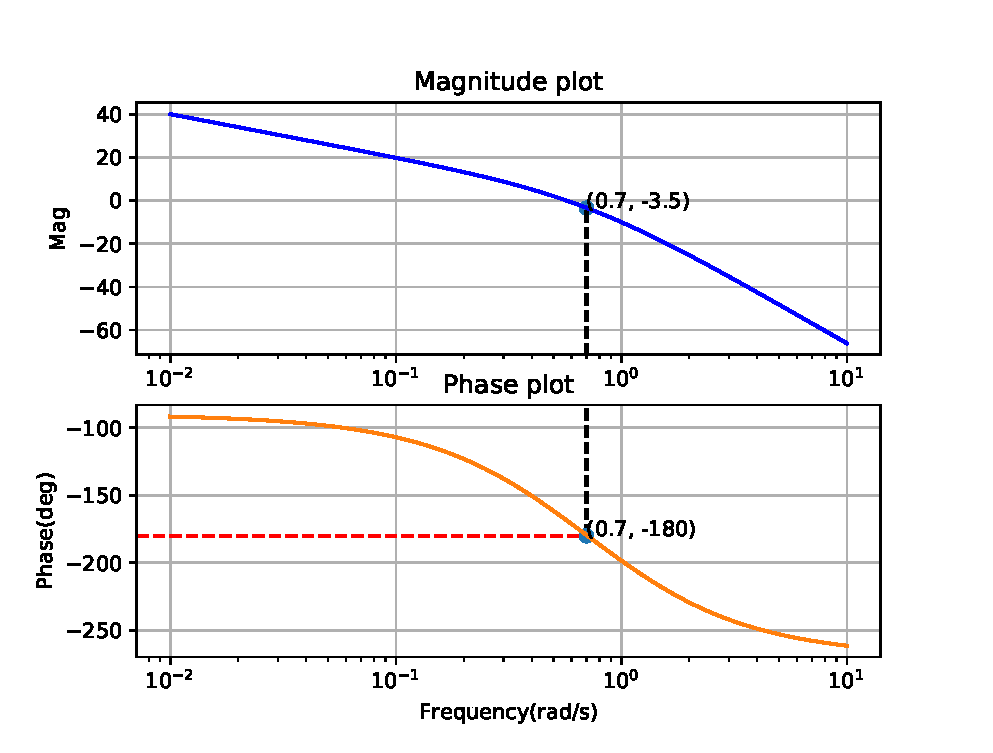
\includegraphics[width=\columnwidth]{./figs/ee18btech11016/ee18btech11016.eps}
	\caption{}
	\label{fig:ee18btech11016}
\end{figure}
From Fig. \ref{fig:ee18btech11016},
\begin{align}
20\log_{10}\abs{G\brak{\j\omega_{pc}}} &= -3.5dB,  \quad \omega_{pc} = -180\degree
\\
\implies  GM &= +3.5dB. 
\end{align}
\item A positive GM indicates closed loop stability with unity feedback.  Verify this for \eqref{ee18btech11016_gs}.
\\
\solution 
The characteristic equation is 
\begin{align}
1+G(s)=0 
\implies 2s^3 + 3s^2 + s + 1 = 0 
\end{align}
Constructing the routh array
\begin{align}
\mydet{s^3\\s^2\\s}
\mydet{2 & 1 & 0 \\ 3 & 1 & 0 \\ (1/3) & 0 & 0}
\\
\mydet{s^3\\s^2\\s\\s^0}
\mydet{2 & 1 & 0 \\ 3 & 1 & 0 \\ (1/3) & 0 & 0 \\ 1 & 0 & 0}
\end{align}\\
%
There are no sign changes in the first column of the routh array. 
$\therefore$ the system is stable.

\item Instead of unity feedback, consider a system with 
%
\begin{align}
H(s)=\frac{1}{s+1}
\end{align}
%
Find the magnitude and phase of $\abs{G\brak{\j\omega}H\brak{\j\omega}}$
\\
\solution 
%
\begin{align}
\because G(s)H(s) & =\frac{1}{s(1+2s)(s+1)^{2}},
\\
G\brak{\j\omega}H\brak{\j\omega} &= \frac{1}{(2\omega^4-4\omega^2) +j(\omega-5\omega^3)}
\\
\implies \angle G\brak{\j\omega}H\brak{\j\omega} &= -tan^{-1}(\frac{\omega-5\omega^3}{2\omega^4-4\omega^2})
\end{align}

\item Compute the open loop gain margin for this system.
\\
\solution 
For $\omega$=$\omega_{pc}$ 

\begin{align}
\text{Im}\cbrak{G\brak{\j\omega}H\brak{\j\omega}}&=0. 
\\
\implies\omega(1-5\omega^2)=0
\\
\implies\omega_{pc} = \frac{1}{\sqrt{5}}
\end{align}
Hence, 
\begin{align}
GM = -20log_{10}|G\brak{\j\omega_{pc}}H\brak{\j\omega_{pc}}| = 20log_{10}k_{g}
\end{align}
where 
\begin{align}
k_{g}&=\frac{1}{|G\brak{\j\omega_{pc}}H\brak{\j\omega_{pc}}|}
\\
&= \frac{ 18}{25} = 2.853dB.
\end{align}
%
Hence $GM < 0$ and the system is unstable.
%
\item Obtain the GM from the Bode plot.
\\
\solution The following code 
\begin{lstlisting}
codes/ee18btech11016_2.py
\end{lstlisting}
%
plots the amplitude and phase of \eqref{ee18btech11016_gs} in Fig. \ref{fig:ee18btech11016_2}.
%
\begin{figure}[htp]
	\centering
	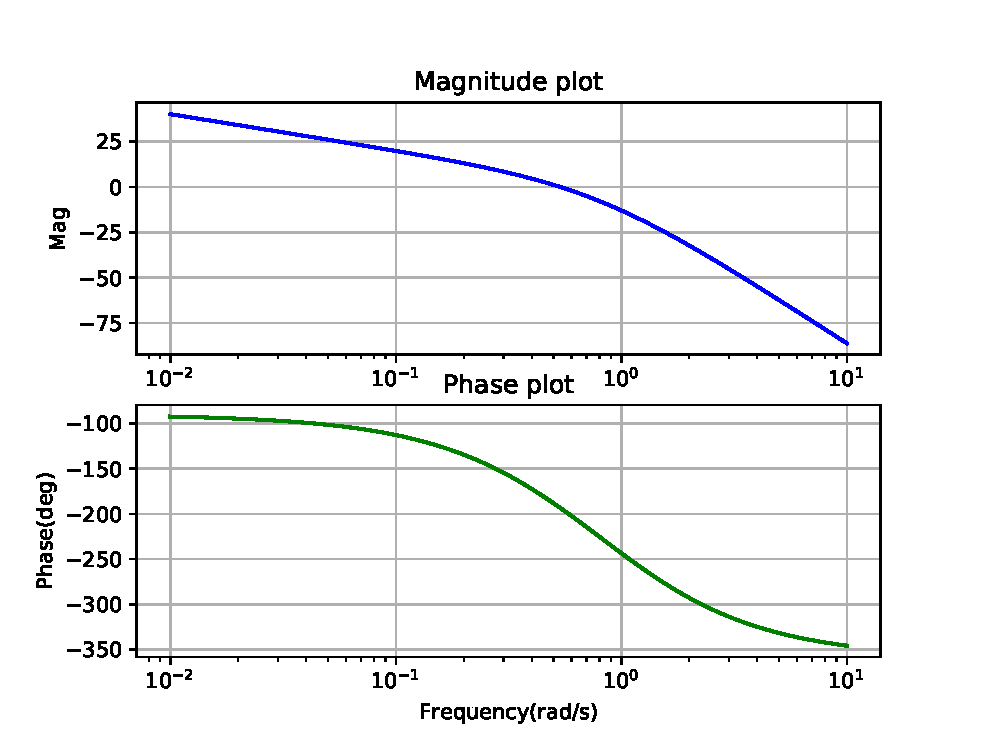
\includegraphics[width=\columnwidth]{./figs/ee18btech11016/ee18btech11016_2.eps}
	\caption{}
	\label{fig:ee18btech11016_2}
\end{figure}
\item Show that the closed loop transfer function 
\begin{align}
T(s) = \frac{1}{1 + (s(1+2s)(1+s)^2)}
\end{align}
%
is unstable using the Routh Hurwitz criterion.
\\
\solution 
The characteristics equation is 
\begin{align}
2s^4 + 5s^3 + 4s^3 + s + 1 = 0 
\end{align}
Constructing routh array for the above,
\begin{align}
\mydet{s^4\\s^3\\s^2}
\mydet{2 & 4 & 1 \\ 5 & 1 & 0 \\ (18/5) & 1 & 0}
\\
\mydet{s^4\\s^3\\s^2\\s}
\mydet{2 & 1 & 0 \\ 3 & 1 & 0 \\ (18/5) & 1 & 0 \\ (-7/18) & 0 & 0}
\\
\mydet{s^4\\s^3\\s^2\\s\\s^0}
\mydet{2 & 1 & 0 \\ 3 & 1 & 0 \\ (18/5) & 1 & 0 \\ (-7/18) & 0 & 0 \\ 1 & 0 & 0}
\end{align}
%
There are 2 sign changes in the first column of the routh array. So, 2 poles lie on right half of s-plane.
Therefore,the system is unstable.
%
\end{enumerate}



\end{enumerate}
\subsection{}
\subsection{}
\subsection{}
\subsection{}
\subsection{Nyquist and Routh-Hurwitz}
\numberwithin{equation}{subsection}
\begin{enumerate}[label=\thesubsection.\arabic*.,ref=\thesubsection.\theenumi]
\numberwithin{equation}{enumi}

\item In the block diagram Fig.\ref{fig:ee18btech11029}  
\begin{align}
G\brak{s} = \frac{K}{\brak{s+4}\brak{s+5}}
\label{ee18btech11034_Gs}
\end{align}
\begin{figure}[!ht]
    \begin{center}
		\resizebox{\columnwidth}{!}{%\begin{enumerate}[label=\thesubsection.\arabic*.,ref=\thesubsection.\theenumi]
%\numberwithin{equation}{enumi}
\item
Sketch the Polar Plot of
\begin{align}
G\brak{s} = \frac{\brak{1+\frac{s}{29}}\brak{1+0.0025s}}{\brak{s^{3}}\brak{1+0.005s}\brak{1+0.001s}}
\end{align}

\solution 
%
The following code generates the polar plot in Fig.   \ref{fig:ee18btech11029}

\begin{lstlisting}
codes/ee18btech11029.py
\end{lstlisting}

\begin{figure}[!h]
\centering
  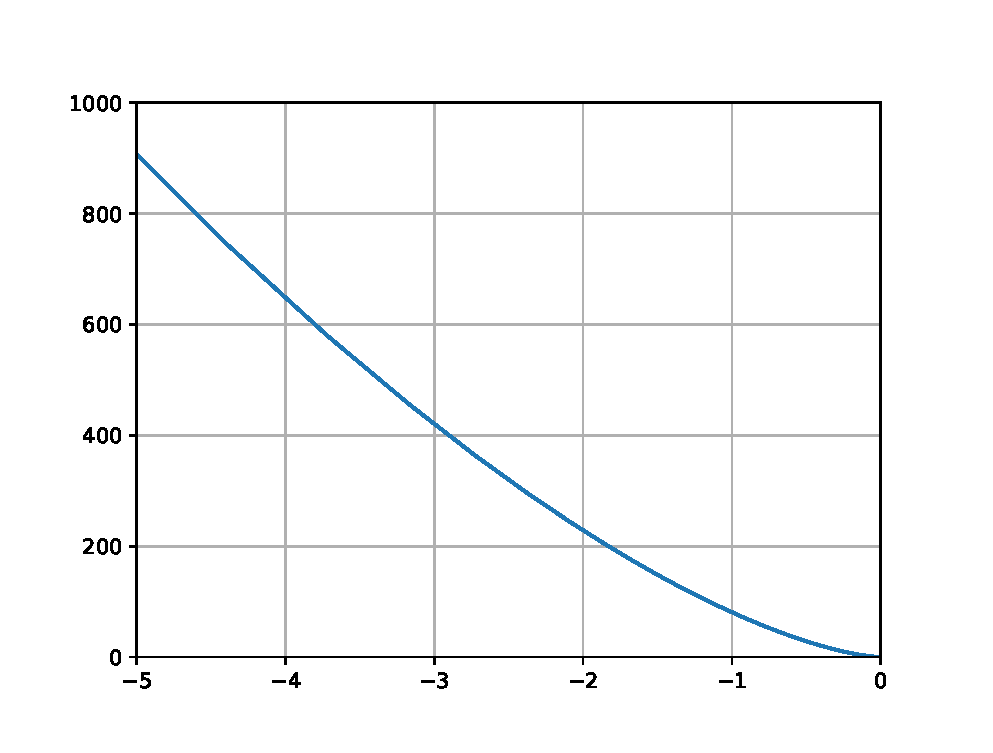
\includegraphics[width=\columnwidth]{./figs/ee18btech11029.eps}
  \caption{}
  \label{fig:ee18btech11029}
\end{figure}

\begin{itemize}
    \item The polar plots use open loop transfer function to determine the stability and hence reference point is shifted to \brak{-1,0}
    \item If \brak{–1,0} is left of the polar plot or \brak{–1,0} is not enclosed, then it is stable
    \item If \brak{–1,0} is on right side of the polar plot or \brak{–1,0} is enclosed by polar plot then it is unstable. 
    \item If \brak{–1,0} is on the polar plot then it is marginally stable
    
\end{itemize}

In Fig.   \ref{fig:ee18btech11029},  \brak{-1,0} is on the polar plot so the system is marginally stable.
   
%\end{enumerate}
}
	\end{center}
\caption{}
\label{fig:ee18btech11029}
\end{figure}
\item Find the range of K for stability by Nyquist criterion

\solution
\begin{figure}[!h]
    \begin{center}
		\resizebox{\columnwidth}{!}{\tikzset{
        block/.style = {draw, rectangle,
            minimum height=1cm,
            minimum width=2cm},
        input/.style = {coordinate,node distance=1cm},
        output/.style = {coordinate,node distance=4cm},
        arrow/.style={draw, -latex,node distance=2cm},
        pinstyle/.style = {pin edge={latex-, black,node distance=2cm}},
        sum/.style = {draw, circle, node distance=1cm},
}

\begin{tikzpicture}[node distance=2.5cm,auto,>=latex']
  \node [input, name=input] {};
  \node [sum, right of=input] (sum) {};
  \node [block, right of = sum] (block1) {$\frac{G(s)}{1+G(s)}$};
  \node [block, right of = block1] (block2) {$\frac{G(s)}{1+G(s)}$};
  \node [output, right of= block2] (output) {};
  \draw [->] (input) -- node {$R(s)\ +$} (sum);
  \draw [->] (sum) -- node {} (block1);
  \draw [->] (block1) -- node {} (block2);
  \draw [->] (block2) -- node [name =y] {$Y(s)$} (output);
  \draw [->] (y) -- ++ (0,-2) -| node [pos=0.99] {$+$} (sum);
\end{tikzpicture}
}
	\end{center}
\caption{}
\label{fig:ee18btech11029_1}
\end{figure}


The open loop transfer function from Fig.\ref{fig:ee18btech11029_1}

\begin{align}
    T\brak{s} =\brak{\frac{\frac{K}{\brak{s+4}\brak{s+5}}}{1+\frac{K}{\brak{s+4}\brak{s+5}}}}^2 
\end{align}


\begin{align}
    T\brak{\j\omega} =\brak{\frac{\frac{K}{\brak{\j\omega+4}\brak{\j\omega+5}}}{1+\frac{K}{\brak{\j\omega+4}\brak{\j\omega+5}}}}^2 
\end{align}




\begin{itemize}
    \item Since it is connected in positive feedback the transfer function cuts at \brak{1,\j0} 
\end{itemize}

\begin{align}
    \implies  \text{Re} \cbrak{T\brak{\j\omega}} &= 1\\
      \implies  \text{Im} \cbrak{T\brak{\j \omega}} &= 0
     \label{eq:ee18btech11029_eq_Re}
\end{align}


\begin{align}
    \brak{\frac{\frac{K}{\brak{\j\omega+4}\brak{\j\omega+5}}}{1+\frac{K}{\brak{\j\omega+4}\brak{\j\omega+5}}}}^2 &= 1+\j0
\end{align}

\begin{align}
    \brak{\j\omega+4}\brak{\j\omega+5}+2K &=0
\end{align}

\begin{align}
    -\omega^2 + 9\j\omega +20+2K &=0 
\end{align}
\\
From  \eqref{eq:ee18btech11029_eq_Re}

\begin{align}
    20 + 2K &= 0\\
    \implies K=-10
\end{align}
The minimum value of stability for the system to be stable is
\begin{align}
    K_{min} > -10
\end{align}
The range of K for which the system is stable is 
\begin{align}
    -10 < K < \infty
\end{align}


\item From the table.\ref{table:ee18btech11029_table1}, 
Stability criterion for K is N+P=Z


\begin{table}[!h]
\centering
%%%%%%%%%%%%%%%%%%%%%%%%%%%%%%%%%%%%%%%%%%%%%%%%%%%%%%%%%%%%%%%%%%%%%%
%%                                                                  %%
%%  This is the header of a LaTeX2e file exported from Gnumeric.    %%
%%                                                                  %%
%%  This file can be compiled as it stands or included in another   %%
%%  LaTeX document. The table is based on the longtable package so  %%
%%  the longtable options (headers, footers...) can be set in the   %%
%%  preamble section below (see PRAMBLE).                           %%
%%                                                                  %%
%%  To include the file in another, the following two lines must be %%
%%  in the including file:                                          %%
%%        \def\inputGnumericTable{}                                 %%
%%  at the beginning of the file and:                               %%
%%        \input{name-of-this-file.tex}                             %%
%%  where the table is to be placed. Note also that the including   %%
%%  file must use the following packages for the table to be        %%
%%  rendered correctly:                                             %%
%%    \usepackage[latin1]{inputenc}                                 %%
%%    \usepackage{color}                                            %%
%%    \usepackage{array}                                            %%
%%    \usepackage{longtable}                                        %%
%%    \usepackage{calc}                                             %%
%%    \usepackage{multirow}                                         %%
%%    \usepackage{hhline}                                           %%
%%    \usepackage{ifthen}                                           %%
%%  optionally (for landscape tables embedded in another document): %%
%%    \usepackage{lscape}                                           %%
%%                                                                  %%
%%%%%%%%%%%%%%%%%%%%%%%%%%%%%%%%%%%%%%%%%%%%%%%%%%%%%%%%%%%%%%%%%%%%%%



%%  This section checks if we are begin input into another file or  %%
%%  the file will be compiled alone. First use a macro taken from   %%
%%  the TeXbook ex 7.7 (suggestion of Han-Wen Nienhuys).            %%
\def\ifundefined#1{\expandafter\ifx\csname#1\endcsname\relax}


%%  Check for the \def token for inputed files. If it is not        %%
%%  defined, the file will be processed as a standalone and the     %%
%%  preamble will be used.                                          %%
\ifundefined{inputGnumericTable}

%%  We must be able to close or not the document at the end.        %%
	\def\gnumericTableEnd{\end{document}}


%%%%%%%%%%%%%%%%%%%%%%%%%%%%%%%%%%%%%%%%%%%%%%%%%%%%%%%%%%%%%%%%%%%%%%
%%                                                                  %%
%%  This is the PREAMBLE. Change these values to get the right      %%
%%  paper size and other niceties.                                  %%
%%                                                                  %%
%%%%%%%%%%%%%%%%%%%%%%%%%%%%%%%%%%%%%%%%%%%%%%%%%%%%%%%%%%%%%%%%%%%%%%

	\documentclass[12pt%
			  %,landscape%
                    ]{report}
       \usepackage[latin1]{inputenc}
       \usepackage{fullpage}
       \usepackage{color}
       \usepackage{array}
       \usepackage{longtable}
       \usepackage{calc}
       \usepackage{multirow}
       \usepackage{hhline}
       \usepackage{ifthen}

	\begin{document}


%%  End of the preamble for the standalone. The next section is for %%
%%  documents which are included into other LaTeX2e files.          %%
\else

%%  We are not a stand alone document. For a regular table, we will %%
%%  have no preamble and only define the closing to mean nothing.   %%
    \def\gnumericTableEnd{}

%%  If we want landscape mode in an embedded document, comment out  %%
%%  the line above and uncomment the two below. The table will      %%
%%  begin on a new page and run in landscape mode.                  %%
%       \def\gnumericTableEnd{\end{landscape}}
%       \begin{landscape}


%%  End of the else clause for this file being \input.              %%
\fi

%%%%%%%%%%%%%%%%%%%%%%%%%%%%%%%%%%%%%%%%%%%%%%%%%%%%%%%%%%%%%%%%%%%%%%
%%                                                                  %%
%%  The rest is the gnumeric table, except for the closing          %%
%%  statement. Changes below will alter the table's appearance.     %%
%%                                                                  %%
%%%%%%%%%%%%%%%%%%%%%%%%%%%%%%%%%%%%%%%%%%%%%%%%%%%%%%%%%%%%%%%%%%%%%%

\providecommand{\gnumericmathit}[1]{#1} 
%%  Uncomment the next line if you would like your numbers to be in %%
%%  italics if they are italizised in the gnumeric table.           %%
%\renewcommand{\gnumericmathit}[1]{\mathit{#1}}
\providecommand{\gnumericPB}[1]%
{\let\gnumericTemp=\\#1\let\\=\gnumericTemp\hspace{0pt}}
 \ifundefined{gnumericTableWidthDefined}
        \newlength{\gnumericTableWidth}
        \newlength{\gnumericTableWidthComplete}
        \newlength{\gnumericMultiRowLength}
        \global\def\gnumericTableWidthDefined{}
 \fi
%% The following setting protects this code from babel shorthands.  %%
 \ifthenelse{\isundefined{\languageshorthands}}{}{\languageshorthands{english}}
%%  The default table format retains the relative column widths of  %%
%%  gnumeric. They can easily be changed to c, r or l. In that case %%
%%  you may want to comment out the next line and uncomment the one %%
%%  thereafter                                                      %%
\providecommand\gnumbox{\makebox[0pt]}
%%\providecommand\gnumbox[1][]{\makebox}

%% to adjust positions in multirow situations                       %%
\setlength{\bigstrutjot}{\jot}
\setlength{\extrarowheight}{\doublerulesep}

%%  The \setlongtables command keeps column widths the same across  %%
%%  pages. Simply comment out next line for varying column widths.  %%
\setlongtables

\setlength\gnumericTableWidth{%
	25pt+%
	25pt+%
	25pt+%
	25pt+%
	50pt+%
0pt}
\def\gumericNumCols{5}
\setlength\gnumericTableWidthComplete{\gnumericTableWidth+%
         \tabcolsep*\gumericNumCols*2+\arrayrulewidth*\gumericNumCols}
\ifthenelse{\lengthtest{\gnumericTableWidthComplete > \linewidth}}%
         {\def\gnumericScale{\ratio{\linewidth-%
                        \tabcolsep*\gumericNumCols*2-%
                        \arrayrulewidth*\gumericNumCols}%
{\gnumericTableWidth}}}%
{\def\gnumericScale{1}}

%%%%%%%%%%%%%%%%%%%%%%%%%%%%%%%%%%%%%%%%%%%%%%%%%%%%%%%%%%%%%%%%%%%%%%
%%                                                                  %%
%% The following are the widths of the various columns. We are      %%
%% defining them here because then they are easier to change.       %%
%% Depending on the cell formats we may use them more than once.    %%
%%                                                                  %%
%%%%%%%%%%%%%%%%%%%%%%%%%%%%%%%%%%%%%%%%%%%%%%%%%%%%%%%%%%%%%%%%%%%%%%

\ifthenelse{\isundefined{\gnumericColA}}{\newlength{\gnumericColA}}{}\settowidth{\gnumericColA}{\begin{tabular}{@{}p{25pt*\gnumericScale}@{}}x\end{tabular}}
\ifthenelse{\isundefined{\gnumericColB}}{\newlength{\gnumericColB}}{}\settowidth{\gnumericColB}{\begin{tabular}{@{}p{25pt*\gnumericScale}@{}}x\end{tabular}}
\ifthenelse{\isundefined{\gnumericColC}}{\newlength{\gnumericColC}}{}\settowidth{\gnumericColC}{\begin{tabular}{@{}p{25pt*\gnumericScale}@{}}x\end{tabular}}
\ifthenelse{\isundefined{\gnumericColD}}{\newlength{\gnumericColD}}{}\settowidth{\gnumericColD}{\begin{tabular}{@{}p{25pt*\gnumericScale}@{}}x\end{tabular}}
\ifthenelse{\isundefined{\gnumericColE}}{\newlength{\gnumericColE}}{}\settowidth{\gnumericColE}{\begin{tabular}{@{}p{50pt*\gnumericScale}@{}}x\end{tabular}}

\begin{tabular}[c]{%
	b{\gnumericColA}%
	b{\gnumericColB}%
	b{\gnumericColC}%
	b{\gnumericColD}%
	b{\gnumericColE}%
	}

%%%%%%%%%%%%%%%%%%%%%%%%%%%%%%%%%%%%%%%%%%%%%%%%%%%%%%%%%%%%%%%%%%%%%%
%%  The longtable options. (Caption, headers... see Goosens, p.124) %%
%	\caption{The Table Caption.}             \\	%
% \hline	% Across the top of the table.
%%  The rest of these options are table rows which are placed on    %%
%%  the first, last or every page. Use \multicolumn if you want.    %%

%%  Header for the first page.                                      %%
%	\multicolumn{3}{c}{The First Header} \\ \hline 
%	\multicolumn{1}{c}{colTag}	%Column 1
%	&\multicolumn{1}{c}{colTag}	%Column 2
%	&\multicolumn{1}{c}{colTag}	\\ \hline %Last column
%	\endfirsthead

%%  The running header definition.                                  %%
%	\hline
%	\multicolumn{3}{l}{\ldots\small\slshape continued} \\ \hline
%	\multicolumn{1}{c}{colTag}	%Column 1
%	&\multicolumn{1}{c}{colTag}	%Column 2
%	&\multicolumn{1}{c}{colTag}	\\ \hline %Last column
%	\endhead

%%  The running footer definition.                                  %%
%	\hline
%	\multicolumn{3}{r}{\small\slshape continued\ldots} \\
%	\endfoot

%%  The ending footer definition.                                   %%
%	\multicolumn{3}{c}{That's all folks} \\ \hline 
%	\endlastfoot
%%%%%%%%%%%%%%%%%%%%%%%%%%%%%%%%%%%%%%%%%%%%%%%%%%%%%%%%%%%%%%%%%%%%%%

\hhline{|-|-|-|-|-}
	 \multicolumn{1}{|p{\gnumericColA}|}%
	{\gnumericPB{\centering}\textbf{K}}
	&\multicolumn{1}{p{\gnumericColB}|}%
	{\gnumericPB{\centering}\textbf{P}}
	&\multicolumn{1}{p{\gnumericColC}|}%
	{\gnumericPB{\centering}\textbf{N}}
	&\multicolumn{1}{p{\gnumericColD}|}%
	{\gnumericPB{\centering}\textbf{Z}}
	&\multicolumn{1}{p{\gnumericColE}|}%
	{\gnumericPB{\raggedright}\textbf{Description}}
	
\\
\hhline{|-----|}
	 \multicolumn{1}{|p{\gnumericColA}|}%
	{\gnumericPB{\centering}-10}
	&\multicolumn{1}{p{\gnumericColB}|}%
	{\gnumericPB{\centering}0}
	&\multicolumn{1}{p{\gnumericColC}|}%
	{\gnumericPB{\centering}0}
	&\multicolumn{1}{p{\gnumericColD}|}%
	{\gnumericPB{\centering}0}
	&\multicolumn{1}{p{\gnumericColE}|}%
	{\gnumericPB{\raggedright}System is marginally stable}
\\
\hhline{|-----|}
	 \multicolumn{1}{|p{\gnumericColA}|}%
	{\gnumericPB{\centering}-9}
	&\multicolumn{1}{p{\gnumericColB}|}%
	{\gnumericPB{\centering}0}
	&\multicolumn{1}{p{\gnumericColC}|}%
	{\gnumericPB{\centering}0}
	&\multicolumn{1}{p{\gnumericColD}|}%
	{\gnumericPB{\centering}0}
	&\multicolumn{1}{p{\gnumericColE}|}%
	{\gnumericPB{\raggedright}System is stable}
\\
\hhline{|-----|}
	 \multicolumn{1}{|p{\gnumericColA}|}%
	{\gnumericPB{\centering}-11}
	&\multicolumn{1}{p{\gnumericColB}|}%
	{\gnumericPB{\centering}0}
	&\multicolumn{1}{p{\gnumericColC}|}%
	{\gnumericPB{\centering}1}
	&\multicolumn{1}{p{\gnumericColD}|}%
	{\gnumericPB{\centering}1}
	&\multicolumn{1}{p{\gnumericColE}|}%
	{\gnumericPB{\raggedright}System is unstable}
\\
\hhline{|-|-|-|-|-|}
\end{tabular}

\ifthenelse{\isundefined{\languageshorthands}}{}{\languageshorthands{\languagename}}
\gnumericTableEnd

\caption{}
\label{table:ee18btech11029_table1}
\end{table}


\item Verify the Nyquist plots by
\begin{lstlisting}
codes/ee18btech11029_1.py
\end{lstlisting}


\begin{figure}[h!]
\centering
  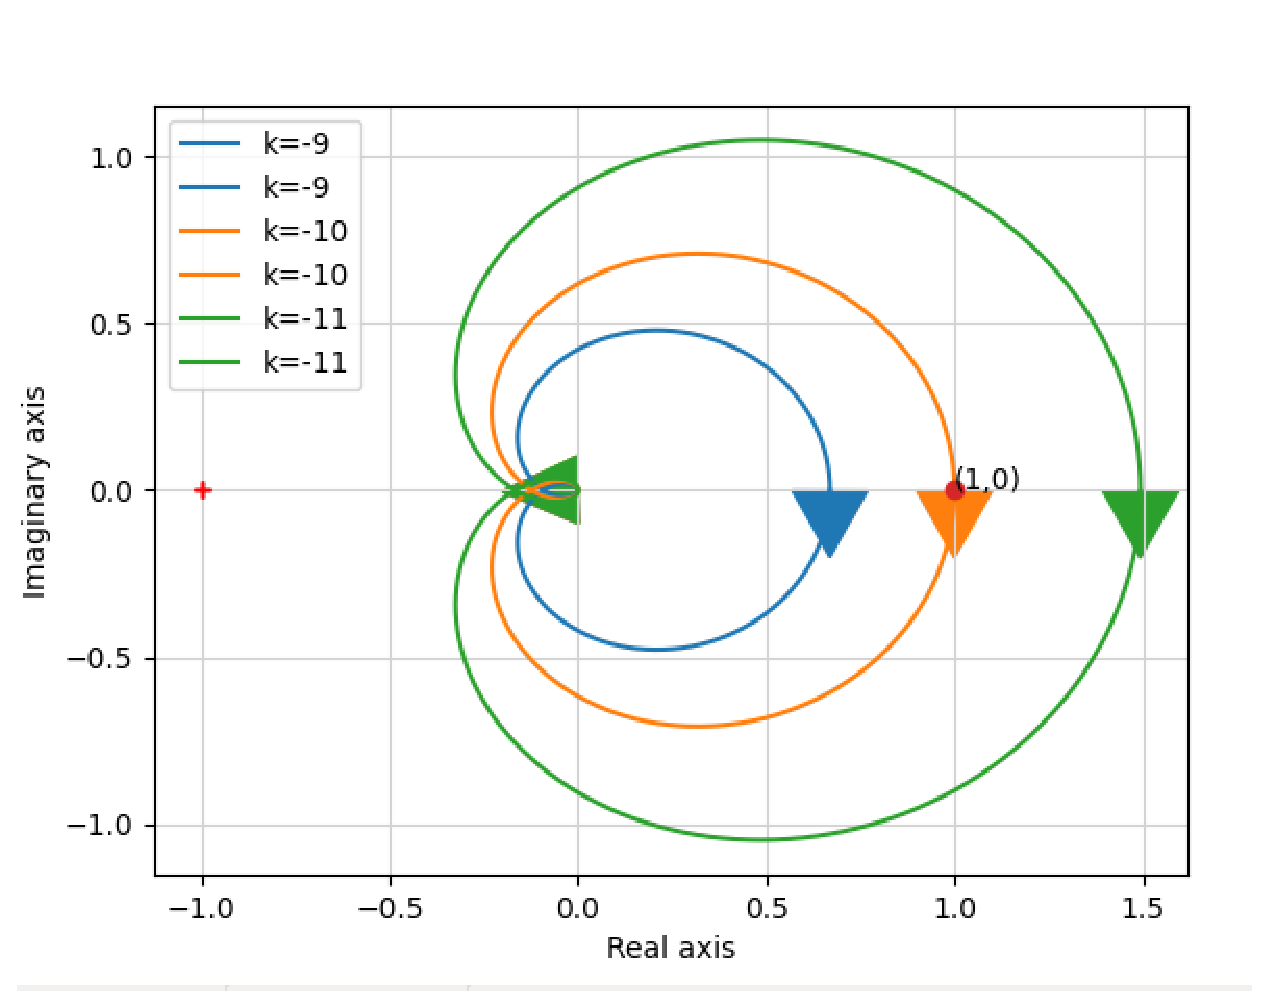
\includegraphics[width=\columnwidth]{./figs/ee18btech11029/Nyquist.eps}
  \caption{Nyquist Plot}
  \label{fig:ee18btech11029_2}
\end{figure}





\item Verify the result using Routh-Hurwitz criterion

\solution The characteristic equation is 
\begin{align}
    1-T\brak{s} &=0\\
    1-\brak{\frac{\frac{K}{\brak{s+4}\brak{s+5}}}{1+\frac{K}{\brak{s+4}\brak{s+5}}}}^2 &=0\\
    1+2\brak{\frac{K}{\brak{s+4}\brak{s+5}}}&=0\\
    s^2+9s+20+2K &= 0
\end{align}

\begin{align}
\mydet{s^2\\s^1\\s^0}
\mydet{1 & 20+2K \\ 9 & 0 \\ 20+2K & 0}
\end{align}
For a system to be stable it should not have any sign changes
\begin{align}
    20+2K >0
\end{align}
This is valid for all positive values of K but the minimum value of K is
\begin{align}
    K>-10
\end{align}
So the range of K for stability is 
\begin{align}
    -10<K<\infty
\end{align}

\item Verify the result by
\begin{lstlisting}
codes/ee18btech11029_2.py
\end{lstlisting}







\end{enumerate}

\subsection{Nyquist}
\numberwithin{equation}{subsection}
%\begin{enumerate}[label=\thesubsection.\arabic*.,ref=\thesubsection.\theenumi]
%\numberwithin{equation}{enumi}

% 
Consider the system shown in Fig. \ref{fig:ee18btech11034}
below. Sketch the nyquist plot of the system when
\begin{enumerate}
\item $G_c(s) = 1$
\item $G_c(s) = 1+\frac{1}{s}$
\end{enumerate} 

and determine the maximum value of $K$ for stability.
Take  
\begin{align}
G\brak{s} = \frac{K}{s\brak{1+s}\brak{1+4s}}
\label{eq:ee18btech11034_Gs}
\end{align}

\begin{figure}[!ht]
	\begin{center}
		
		\resizebox{\columnwidth}{!}{\tikzset{
        block/.style = {draw, rectangle,
            minimum height=1cm,
            minimum width=2cm},
        input/.style = {coordinate,node distance=1cm},
        output/.style = {coordinate,node distance=4cm},
        arrow/.style={draw, -latex,node distance=2cm},
        pinstyle/.style = {pin edge={latex-, black,node distance=2cm}},
        sum/.style = {draw, circle, node distance=1cm},
}

\begin{tikzpicture}[node distance=2.5cm,auto,>=latex']
  \node [input, name=input] {};
  \node [sum, right of=input] (sum) {};
  \node [block, right of = sum] (block1) {$G_c(s)$};
  \node [block, right of = block1] (block2) {$G(s)$};
  \node [output, right of= block2] (output) {};
  \draw [->] (input) -- node {$R(s)\ +$} (sum);
  \draw [->] (sum) -- node {} (block1);
  \draw [->] (block1) -- node {} (block2);
  \draw [->] (block2) -- node [name =y] {$Y(s)$} (output);
  \draw [->] (y) -- ++ (0,-2) -| node [pos=0.99] {$-$} (sum);
\end{tikzpicture}}
	\end{center}
\caption{}
\label{fig:ee18btech11034}
\end{figure}

\solution
 For $G_{c}\brak{s}$ = 1,

The open loop transfer function is 
\begin{align}
    G_{c}\brak{s}G\brak{s} = \frac{K}{s\brak{1+s}\brak{1+4s}}
\end{align}

\begin{align}
    G_{c}\brak{\j\omega}G\brak{\j\omega} &= \frac{K}{{\j\omega}\brak{1+\j\omega}\brak{1+4\j\omega}}
    \\
    &= \frac{K}{{\j\omega}\brak{1-4\omega^2+5\j\omega}}
    \\
    &= \frac{K\brak{-5\omega-\j\brak{1-4\omega^2}}}{{\omega}\brak{\brak{1-4\omega^2}^2+25\omega^2}}
    \end{align}
The maximum K for stability is where the nyquist plot of open loop transfer function cuts the coordinate \brak{-1,\j0}


\begin{align}
 \implies    \text{Re} \cbrak{G\brak{\j \omega}G_{c}\brak{\j\omega}} &= -1
 \label{eq:ee18btech11034_eq_Re}
 \\
 \implies \text{Im} \cbrak{G\brak{\j \omega}G_{c}\brak{\j\omega}} &= 0
 \label{eq:ee18btech11034_eq_Im}
\end{align}

\begin{align}
 \implies    \text{Re} \cbrak{G\brak{\j \omega}G_{c}\brak{\j\omega}} &= \frac{-5K\omega}{{\omega}\brak{\brak{1-4\omega^2}^2+25\omega^2}}
 \label{eq:ee18btech11034_eq_1_Re}
 \\
 \implies \text{Im} \cbrak{G\brak{\j \omega}G_{c}\brak{\j\omega}} &= \frac{-K\brak{1-4\omega^2}}{{\omega}\brak{\brak{1-4\omega^2}^2+25\omega^2}}
 \label{eq:ee18btech11034_eq_1_Im}
\end{align}

From \eqref{eq:ee18btech11034_eq_1_Im} and \eqref{eq:ee18btech11034_eq_Im}
\begin{align}
    1-4\omega^2 = 0
    \implies \omega = \frac{1}{2} 
\end{align}
From  \eqref{eq:ee18btech11034_eq_1_Re},\eqref{eq:ee18btech11034_eq_Re} and substituting $\omega = \frac{1}{2}$
\begin{align}
    \frac{-5K\brak{\frac{1}{2}}}{\brak{\frac{1}{2}}\brak{\frac{25}{4}}} = -1
    \implies K = \frac{5}{4} = 1.25
\end{align}

For $K < 0$ the system with negative feedback is unstable the range of K is 
\begin{align}
    0 < K < \frac{5}{4}
\end{align}
 Sketching the Nyquist plot for $G(s)G_c(s)$ in Fig. \ref{fig:ee18btech11034_1}
The following code gives the nyquist plot
\begin{lstlisting}
codes/ee18btech11034/ee18btech11034_1.py
\end{lstlisting}

\begin{figure}[!h]
\centering
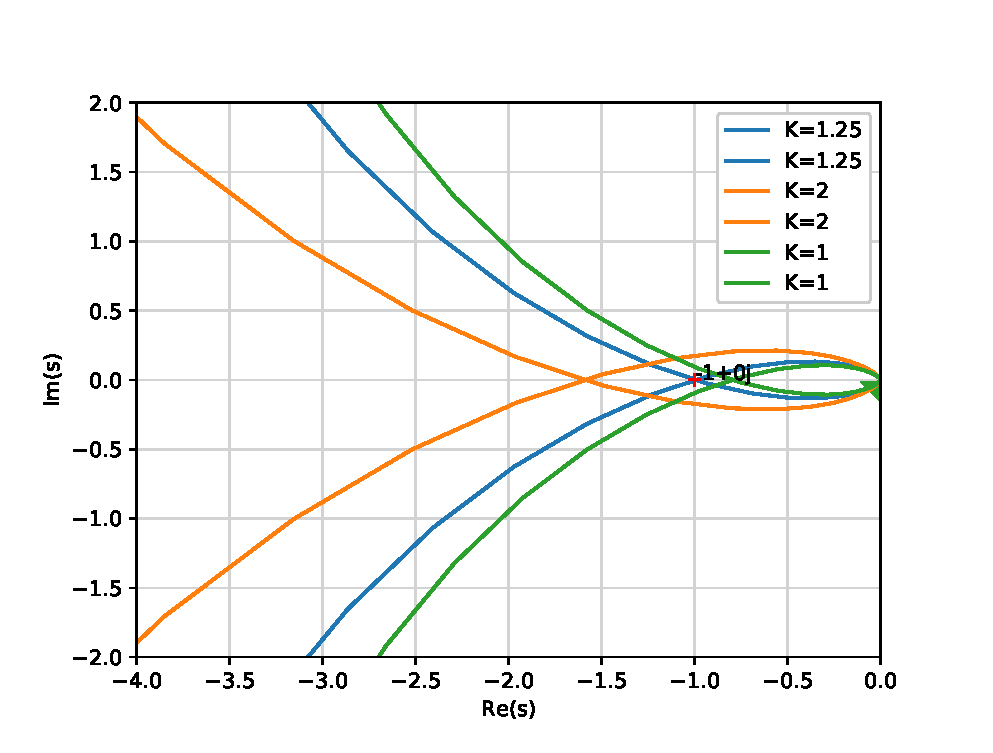
\includegraphics[width=\columnwidth]{./figs/ee18btech11034/ee18btech11034_1.eps}
\caption{}
\label{fig:ee18btech11034_1}
\end{figure}
 Stability Criterian for K
\begin{align}
    N + P = Z
    \label{eq:ee18btech11034_Z}
\end{align}
\begin{table}[!ht]
\centering
%%%%%%%%%%%%%%%%%%%%%%%%%%%%%%%%%%%%%%%%%%%%%%%%%%%%%%%%%%%%%%%%%%%%%%
%%                                                                  %%
%%  This is the header of a LaTeX2e file exported from Gnumeric.    %%
%%                                                                  %%
%%  This file can be compiled as it stands or included in another   %%
%%  LaTeX document. The table is based on the longtable package so  %%
%%  the longtable options (headers, footers...) can be set in the   %%
%%  preamble section below (see PRAMBLE).                           %%
%%                                                                  %%
%%  To include the file in another, the following two lines must be %%
%%  in the including file:                                          %%
%%        \def\inputGnumericTable{}                                 %%
%%  at the beginning of the file and:                               %%
%%        \input{name-of-this-file.tex}                             %%
%%  where the table is to be placed. Note also that the including   %%
%%  file must use the following packages for the table to be        %%
%%  rendered correctly:                                             %%
%%    \usepackage[latin1]{inputenc}                                 %%
%%    \usepackage{color}                                            %%
%%    \usepackage{array}                                            %%
%%    \usepackage{longtable}                                        %%
%%    \usepackage{calc}                                             %%
%%    \usepackage{multirow}                                         %%
%%    \usepackage{hhline}                                           %%
%%    \usepackage{ifthen}                                           %%
%%  optionally (for landscape tables embedded in another document): %%
%%    \usepackage{lscape}                                           %%
%%                                                                  %%
%%%%%%%%%%%%%%%%%%%%%%%%%%%%%%%%%%%%%%%%%%%%%%%%%%%%%%%%%%%%%%%%%%%%%%



%%  This section checks if we are begin input into another file or  %%
%%  the file will be compiled alone. First use a macro taken from   %%
%%  the TeXbook ex 7.7 (suggestion of Han-Wen Nienhuys).            %%
\def\ifundefined#1{\expandafter\ifx\csname#1\endcsname\relax}


%%  Check for the \def token for inputed files. If it is not        %%
%%  defined, the file will be processed as a standalone and the     %%
%%  preamble will be used.                                          %%
\ifundefined{inputGnumericTable}

%%  We must be able to close or not the document at the end.        %%
	\def\gnumericTableEnd{\end{document}}


%%%%%%%%%%%%%%%%%%%%%%%%%%%%%%%%%%%%%%%%%%%%%%%%%%%%%%%%%%%%%%%%%%%%%%
%%                                                                  %%
%%  This is the PREAMBLE. Change these values to get the right      %%
%%  paper size and other niceties.                                  %%
%%                                                                  %%
%%%%%%%%%%%%%%%%%%%%%%%%%%%%%%%%%%%%%%%%%%%%%%%%%%%%%%%%%%%%%%%%%%%%%%

	\documentclass[12pt%
			  %,landscape%
                    ]{report}
       \usepackage[latin1]{inputenc}
       \usepackage{fullpage}
       \usepackage{color}
       \usepackage{array}
       \usepackage{longtable}
       \usepackage{calc}
       \usepackage{multirow}
       \usepackage{hhline}
       \usepackage{ifthen}

	\begin{document}


%%  End of the preamble for the standalone. The next section is for %%
%%  documents which are included into other LaTeX2e files.          %%
\else

%%  We are not a stand alone document. For a regular table, we will %%
%%  have no preamble and only define the closing to mean nothing.   %%
    \def\gnumericTableEnd{}

%%  If we want landscape mode in an embedded document, comment out  %%
%%  the line above and uncomment the two below. The table will      %%
%%  begin on a new page and run in landscape mode.                  %%
%       \def\gnumericTableEnd{\end{landscape}}
%       \begin{landscape}


%%  End of the else clause for this file being \input.              %%
\fi

%%%%%%%%%%%%%%%%%%%%%%%%%%%%%%%%%%%%%%%%%%%%%%%%%%%%%%%%%%%%%%%%%%%%%%
%%                                                                  %%
%%  The rest is the gnumeric table, except for the closing          %%
%%  statement. Changes below will alter the table's appearance.     %%
%%                                                                  %%
%%%%%%%%%%%%%%%%%%%%%%%%%%%%%%%%%%%%%%%%%%%%%%%%%%%%%%%%%%%%%%%%%%%%%%

\providecommand{\gnumericmathit}[1]{#1} 
%%  Uncomment the next line if you would like your numbers to be in %%
%%  italics if they are italizised in the gnumeric table.           %%
%\renewcommand{\gnumericmathit}[1]{\mathit{#1}}
\providecommand{\gnumericPB}[1]%
{\let\gnumericTemp=\\#1\let\\=\gnumericTemp\hspace{0pt}}
 \ifundefined{gnumericTableWidthDefined}
        \newlength{\gnumericTableWidth}
        \newlength{\gnumericTableWidthComplete}
        \newlength{\gnumericMultiRowLength}
        \global\def\gnumericTableWidthDefined{}
 \fi
%% The following setting protects this code from babel shorthands.  %%
 \ifthenelse{\isundefined{\languageshorthands}}{}{\languageshorthands{english}}
%%  The default table format retains the relative column widths of  %%
%%  gnumeric. They can easily be changed to c, r or l. In that case %%
%%  you may want to comment out the next line and uncomment the one %%
%%  thereafter                                                      %%
\providecommand\gnumbox{\makebox[0pt]}
%%\providecommand\gnumbox[1][]{\makebox}

%% to adjust positions in multirow situations                       %%
\setlength{\bigstrutjot}{\jot}
\setlength{\extrarowheight}{\doublerulesep}

%%  The \setlongtables command keeps column widths the same across  %%
%%  pages. Simply comment out next line for varying column widths.  %%
\setlongtables

\setlength\gnumericTableWidth{%
	25pt+%
	25pt+%
	25pt+%
	25pt+%
	50pt+%
0pt}
\def\gumericNumCols{5}
\setlength\gnumericTableWidthComplete{\gnumericTableWidth+%
         \tabcolsep*\gumericNumCols*2+\arrayrulewidth*\gumericNumCols}
\ifthenelse{\lengthtest{\gnumericTableWidthComplete > \linewidth}}%
         {\def\gnumericScale{\ratio{\linewidth-%
                        \tabcolsep*\gumericNumCols*2-%
                        \arrayrulewidth*\gumericNumCols}%
{\gnumericTableWidth}}}%
{\def\gnumericScale{1}}

%%%%%%%%%%%%%%%%%%%%%%%%%%%%%%%%%%%%%%%%%%%%%%%%%%%%%%%%%%%%%%%%%%%%%%
%%                                                                  %%
%% The following are the widths of the various columns. We are      %%
%% defining them here because then they are easier to change.       %%
%% Depending on the cell formats we may use them more than once.    %%
%%                                                                  %%
%%%%%%%%%%%%%%%%%%%%%%%%%%%%%%%%%%%%%%%%%%%%%%%%%%%%%%%%%%%%%%%%%%%%%%

\ifthenelse{\isundefined{\gnumericColA}}{\newlength{\gnumericColA}}{}\settowidth{\gnumericColA}{\begin{tabular}{@{}p{25pt*\gnumericScale}@{}}x\end{tabular}}
\ifthenelse{\isundefined{\gnumericColB}}{\newlength{\gnumericColB}}{}\settowidth{\gnumericColB}{\begin{tabular}{@{}p{25pt*\gnumericScale}@{}}x\end{tabular}}
\ifthenelse{\isundefined{\gnumericColC}}{\newlength{\gnumericColC}}{}\settowidth{\gnumericColC}{\begin{tabular}{@{}p{25pt*\gnumericScale}@{}}x\end{tabular}}
\ifthenelse{\isundefined{\gnumericColD}}{\newlength{\gnumericColD}}{}\settowidth{\gnumericColD}{\begin{tabular}{@{}p{25pt*\gnumericScale}@{}}x\end{tabular}}
\ifthenelse{\isundefined{\gnumericColE}}{\newlength{\gnumericColE}}{}\settowidth{\gnumericColE}{\begin{tabular}{@{}p{50pt*\gnumericScale}@{}}x\end{tabular}}

\begin{tabular}[c]{%
	b{\gnumericColA}%
	b{\gnumericColB}%
	b{\gnumericColC}%
	b{\gnumericColD}%
	b{\gnumericColE}%
	}

%%%%%%%%%%%%%%%%%%%%%%%%%%%%%%%%%%%%%%%%%%%%%%%%%%%%%%%%%%%%%%%%%%%%%%
%%  The longtable options. (Caption, headers... see Goosens, p.124) %%
%	\caption{The Table Caption.}             \\	%
% \hline	% Across the top of the table.
%%  The rest of these options are table rows which are placed on    %%
%%  the first, last or every page. Use \multicolumn if you want.    %%

%%  Header for the first page.                                      %%
%	\multicolumn{3}{c}{The First Header} \\ \hline 
%	\multicolumn{1}{c}{colTag}	%Column 1
%	&\multicolumn{1}{c}{colTag}	%Column 2
%	&\multicolumn{1}{c}{colTag}	\\ \hline %Last column
%	\endfirsthead

%%  The running header definition.                                  %%
%	\hline
%	\multicolumn{3}{l}{\ldots\small\slshape continued} \\ \hline
%	\multicolumn{1}{c}{colTag}	%Column 1
%	&\multicolumn{1}{c}{colTag}	%Column 2
%	&\multicolumn{1}{c}{colTag}	\\ \hline %Last column
%	\endhead

%%  The running footer definition.                                  %%
%	\hline
%	\multicolumn{3}{r}{\small\slshape continued\ldots} \\
%	\endfoot

%%  The ending footer definition.                                   %%
%	\multicolumn{3}{c}{That's all folks} \\ \hline 
%	\endlastfoot
%%%%%%%%%%%%%%%%%%%%%%%%%%%%%%%%%%%%%%%%%%%%%%%%%%%%%%%%%%%%%%%%%%%%%%

\hhline{|-|-|-|-|-}
	 \multicolumn{1}{|p{\gnumericColA}|}%
	{\gnumericPB{\centering}\textbf{K}}
	&\multicolumn{1}{p{\gnumericColB}|}%
	{\gnumericPB{\centering}\textbf{P}}
	&\multicolumn{1}{p{\gnumericColC}|}%
	{\gnumericPB{\centering}\textbf{N}}
	&\multicolumn{1}{p{\gnumericColD}|}%
	{\gnumericPB{\centering}\textbf{Z}}
	&\multicolumn{1}{p{\gnumericColE}|}%
	{\gnumericPB{\raggedright}\textbf{Description}}
	
\\
\hhline{|-----|}
	 \multicolumn{1}{|p{\gnumericColA}|}%
	{\gnumericPB{\centering}1.25}
	&\multicolumn{1}{p{\gnumericColB}|}%
	{\gnumericPB{\centering}0}
	&\multicolumn{1}{p{\gnumericColC}|}%
	{\gnumericPB{\centering}0}
	&\multicolumn{1}{p{\gnumericColD}|}%
	{\gnumericPB{\centering}0}
	&\multicolumn{1}{p{\gnumericColE}|}%
	{\gnumericPB{\raggedright}System is marginally stable}
\\
\hhline{|-----|}
	 \multicolumn{1}{|p{\gnumericColA}|}%
	{\gnumericPB{\centering}2}
	&\multicolumn{1}{p{\gnumericColB}|}%
	{\gnumericPB{\centering}0}
	&\multicolumn{1}{p{\gnumericColC}|}%
	{\gnumericPB{\centering}1}
	&\multicolumn{1}{p{\gnumericColD}|}%
	{\gnumericPB{\centering}1}
	&\multicolumn{1}{p{\gnumericColE}|}%
	{\gnumericPB{\raggedright}System is unstable}
\\
\hhline{|-----|}
	 \multicolumn{1}{|p{\gnumericColA}|}%
	{\gnumericPB{\centering}1}
	&\multicolumn{1}{p{\gnumericColB}|}%
	{\gnumericPB{\centering}0}
	&\multicolumn{1}{p{\gnumericColC}|}%
	{\gnumericPB{\centering}0}
	&\multicolumn{1}{p{\gnumericColD}|}%
	{\gnumericPB{\centering}0}
	&\multicolumn{1}{p{\gnumericColE}|}%
	{\gnumericPB{\raggedright}System is stable}
\\
\hhline{|-|-|-|-|-|}
\end{tabular}

\ifthenelse{\isundefined{\languageshorthands}}{}{\languageshorthands{\languagename}}
\gnumericTableEnd
\caption{}
\label{table:ee18btech11034_table1}
\end{table}

From the Fig.\ref{fig:ee18btech11034_1}  
\begin{align}
 K_{max} = \frac{5}{4}  
\end{align}


\solution
For $G_{c}\brak{s} = \frac{1+s}{s}$,

the open loop transfer function is 
\begin{align}
    G_{c}\brak{s}G\brak{s} &= \frac{K\brak{s+1}}{s^2\brak{1+s}\brak{1+4s}}
\end{align}
\begin{align}
    G_{c}\brak{s}G\brak{s} &= \frac{K}{s^2\brak{1+4s}}
\end{align}
\begin{align}
    G_{c}\brak{\j\omega}G\brak{\j\omega} &= \frac{K}{\brak{\j\omega}^2\brak{1+4\j\omega}}
    \\
    &= \frac{\frac{-K}{\omega^2}\brak{1-4\j\omega}}{1+16\omega^2}
\end{align}
From \eqref{eq:ee18btech11034_eq_Im}
\begin{align}
    \implies \text{Im} \cbrak{G\brak{\j \omega}G_{c}\brak{\j\omega}} &= \frac{4K}{{\omega}\brak{1+16\omega^2}} &= 0
\end{align}
This is possible when 
\begin{align}
    K = 0
    \label{eq:ee18btech11034_3}
\end{align}

The system is unstable for both 
\begin{align}
    K &< 0
\end{align}
\begin{align}
    K &> 0
\end{align}

 Sketching the Nyquist plot for $G(s)G_c(s)$ in Fig. \ref{fig:ee18btech11034_2}
The following code gives the nyquist plot
\begin{lstlisting}
codes/ee18btech11034/ee18btech11034_2.py
\end{lstlisting}
\begin{figure}[!h]
\centering
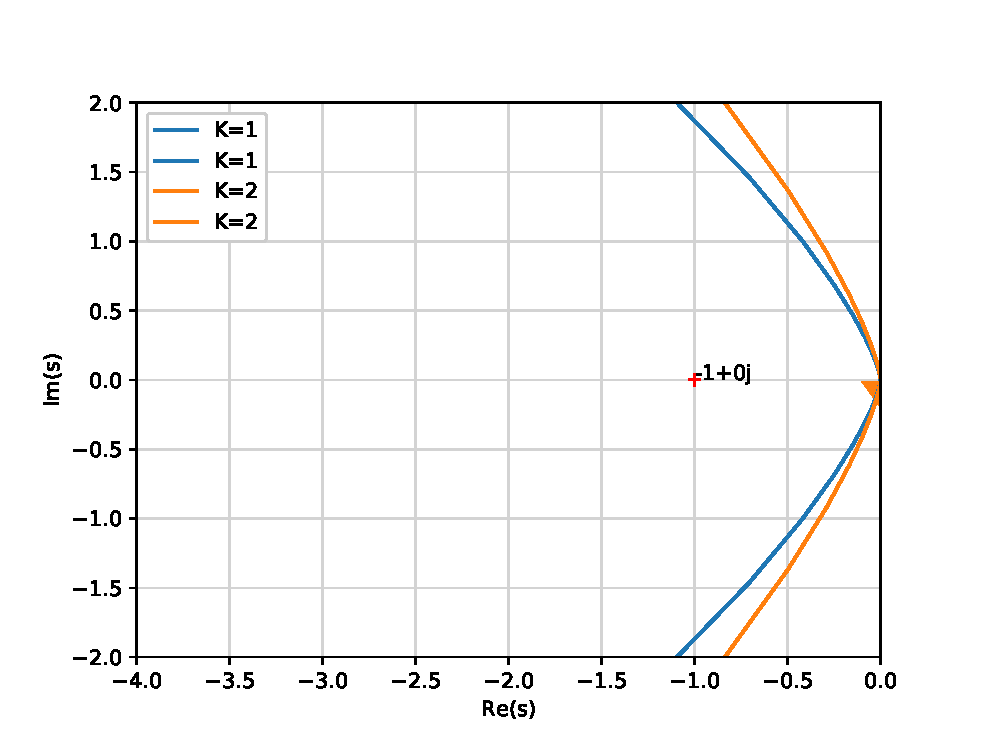
\includegraphics[width=\columnwidth]{./figs/ee18btech11034/ee18btech11034_2.eps}
\caption{}
\label{fig:ee18btech11034_2}
\end{figure}
From \eqref{eq:ee18btech11034_Z}

\begin{table}[!ht]
\centering
%%%%%%%%%%%%%%%%%%%%%%%%%%%%%%%%%%%%%%%%%%%%%%%%%%%%%%%%%%%%%%%%%%%%%%
%%                                                                  %%
%%  This is the header of a LaTeX2e file exported from Gnumeric.    %%
%%                                                                  %%
%%  This file can be compiled as it stands or included in another   %%
%%  LaTeX document. The table is based on the longtable package so  %%
%%  the longtable options (headers, footers...) can be set in the   %%
%%  preamble section below (see PRAMBLE).                           %%
%%                                                                  %%
%%  To include the file in another, the following two lines must be %%
%%  in the including file:                                          %%
%%        \def\inputGnumericTable{}                                 %%
%%  at the beginning of the file and:                               %%
%%        \input{name-of-this-file.tex}                             %%
%%  where the table is to be placed. Note also that the including   %%
%%  file must use the following packages for the table to be        %%
%%  rendered correctly:                                             %%
%%    \usepackage[latin1]{inputenc}                                 %%
%%    \usepackage{color}                                            %%
%%    \usepackage{array}                                            %%
%%    \usepackage{longtable}                                        %%
%%    \usepackage{calc}                                             %%
%%    \usepackage{multirow}                                         %%
%%    \usepackage{hhline}                                           %%
%%    \usepackage{ifthen}                                           %%
%%  optionally (for landscape tables embedded in another document): %%
%%    \usepackage{lscape}                                           %%
%%                                                                  %%
%%%%%%%%%%%%%%%%%%%%%%%%%%%%%%%%%%%%%%%%%%%%%%%%%%%%%%%%%%%%%%%%%%%%%%



%%  This section checks if we are begin input into another file or  %%
%%  the file will be compiled alone. First use a macro taken from   %%
%%  the TeXbook ex 7.7 (suggestion of Han-Wen Nienhuys).            %%
\def\ifundefined#1{\expandafter\ifx\csname#1\endcsname\relax}


%%  Check for the \def token for inputed files. If it is not        %%
%%  defined, the file will be processed as a standalone and the     %%
%%  preamble will be used.                                          %%
\ifundefined{inputGnumericTable}

%%  We must be able to close or not the document at the end.        %%
	\def\gnumericTableEnd{\end{document}}


%%%%%%%%%%%%%%%%%%%%%%%%%%%%%%%%%%%%%%%%%%%%%%%%%%%%%%%%%%%%%%%%%%%%%%
%%                                                                  %%
%%  This is the PREAMBLE. Change these values to get the right      %%
%%  paper size and other niceties.                                  %%
%%                                                                  %%
%%%%%%%%%%%%%%%%%%%%%%%%%%%%%%%%%%%%%%%%%%%%%%%%%%%%%%%%%%%%%%%%%%%%%%

	\documentclass[12pt%
			  %,landscape%
                    ]{report}
       \usepackage[latin1]{inputenc}
       \usepackage{fullpage}
       \usepackage{color}
       \usepackage{array}
       \usepackage{longtable}
       \usepackage{calc}
       \usepackage{multirow}
       \usepackage{hhline}
       \usepackage{ifthen}

	\begin{document}


%%  End of the preamble for the standalone. The next section is for %%
%%  documents which are included into other LaTeX2e files.          %%
\else

%%  We are not a stand alone document. For a regular table, we will %%
%%  have no preamble and only define the closing to mean nothing.   %%
    \def\gnumericTableEnd{}

%%  If we want landscape mode in an embedded document, comment out  %%
%%  the line above and uncomment the two below. The table will      %%
%%  begin on a new page and run in landscape mode.                  %%
%       \def\gnumericTableEnd{\end{landscape}}
%       \begin{landscape}


%%  End of the else clause for this file being \input.              %%
\fi

%%%%%%%%%%%%%%%%%%%%%%%%%%%%%%%%%%%%%%%%%%%%%%%%%%%%%%%%%%%%%%%%%%%%%%
%%                                                                  %%
%%  The rest is the gnumeric table, except for the closing          %%
%%  statement. Changes below will alter the table's appearance.     %%
%%                                                                  %%
%%%%%%%%%%%%%%%%%%%%%%%%%%%%%%%%%%%%%%%%%%%%%%%%%%%%%%%%%%%%%%%%%%%%%%

\providecommand{\gnumericmathit}[1]{#1} 
%%  Uncomment the next line if you would like your numbers to be in %%
%%  italics if they are italizised in the gnumeric table.           %%
%\renewcommand{\gnumericmathit}[1]{\mathit{#1}}
\providecommand{\gnumericPB}[1]%
{\let\gnumericTemp=\\#1\let\\=\gnumericTemp\hspace{0pt}}
 \ifundefined{gnumericTableWidthDefined}
        \newlength{\gnumericTableWidth}
        \newlength{\gnumericTableWidthComplete}
        \newlength{\gnumericMultiRowLength}
        \global\def\gnumericTableWidthDefined{}
 \fi
%% The following setting protects this code from babel shorthands.  %%
 \ifthenelse{\isundefined{\languageshorthands}}{}{\languageshorthands{english}}
%%  The default table format retains the relative column widths of  %%
%%  gnumeric. They can easily be changed to c, r or l. In that case %%
%%  you may want to comment out the next line and uncomment the one %%
%%  thereafter                                                      %%
\providecommand\gnumbox{\makebox[0pt]}
%%\providecommand\gnumbox[1][]{\makebox}

%% to adjust positions in multirow situations                       %%
\setlength{\bigstrutjot}{\jot}
\setlength{\extrarowheight}{\doublerulesep}

%%  The \setlongtables command keeps column widths the same across  %%
%%  pages. Simply comment out next line for varying column widths.  %%
\setlongtables

\setlength\gnumericTableWidth{%
	25pt+%
	25pt+%
	25pt+%
	25pt+%
	50pt+%
0pt}
\def\gumericNumCols{5}
\setlength\gnumericTableWidthComplete{\gnumericTableWidth+%
         \tabcolsep*\gumericNumCols*2+\arrayrulewidth*\gumericNumCols}
\ifthenelse{\lengthtest{\gnumericTableWidthComplete > \linewidth}}%
         {\def\gnumericScale{\ratio{\linewidth-%
                        \tabcolsep*\gumericNumCols*2-%
                        \arrayrulewidth*\gumericNumCols}%
{\gnumericTableWidth}}}%
{\def\gnumericScale{1}}

%%%%%%%%%%%%%%%%%%%%%%%%%%%%%%%%%%%%%%%%%%%%%%%%%%%%%%%%%%%%%%%%%%%%%%
%%                                                                  %%
%% The following are the widths of the various columns. We are      %%
%% defining them here because then they are easier to change.       %%
%% Depending on the cell formats we may use them more than once.    %%
%%                                                                  %%
%%%%%%%%%%%%%%%%%%%%%%%%%%%%%%%%%%%%%%%%%%%%%%%%%%%%%%%%%%%%%%%%%%%%%%

\ifthenelse{\isundefined{\gnumericColA}}{\newlength{\gnumericColA}}{}\settowidth{\gnumericColA}{\begin{tabular}{@{}p{25pt*\gnumericScale}@{}}x\end{tabular}}
\ifthenelse{\isundefined{\gnumericColB}}{\newlength{\gnumericColB}}{}\settowidth{\gnumericColB}{\begin{tabular}{@{}p{25pt*\gnumericScale}@{}}x\end{tabular}}
\ifthenelse{\isundefined{\gnumericColC}}{\newlength{\gnumericColC}}{}\settowidth{\gnumericColC}{\begin{tabular}{@{}p{25pt*\gnumericScale}@{}}x\end{tabular}}
\ifthenelse{\isundefined{\gnumericColD}}{\newlength{\gnumericColD}}{}\settowidth{\gnumericColD}{\begin{tabular}{@{}p{25pt*\gnumericScale}@{}}x\end{tabular}}
\ifthenelse{\isundefined{\gnumericColE}}{\newlength{\gnumericColE}}{}\settowidth{\gnumericColE}{\begin{tabular}{@{}p{50pt*\gnumericScale}@{}}x\end{tabular}}

\begin{tabular}[c]{%
	b{\gnumericColA}%
	b{\gnumericColB}%
	b{\gnumericColC}%
	b{\gnumericColD}%
	b{\gnumericColE}%
	}

%%%%%%%%%%%%%%%%%%%%%%%%%%%%%%%%%%%%%%%%%%%%%%%%%%%%%%%%%%%%%%%%%%%%%%
%%  The longtable options. (Caption, headers... see Goosens, p.124) %%
%	\caption{The Table Caption.}             \\	%
% \hline	% Across the top of the table.
%%  The rest of these options are table rows which are placed on    %%
%%  the first, last or every page. Use \multicolumn if you want.    %%

%%  Header for the first page.                                      %%
%	\multicolumn{3}{c}{The First Header} \\ \hline 
%	\multicolumn{1}{c}{colTag}	%Column 1
%	&\multicolumn{1}{c}{colTag}	%Column 2
%	&\multicolumn{1}{c}{colTag}	\\ \hline %Last column
%	\endfirsthead

%%  The running header definition.                                  %%
%	\hline
%	\multicolumn{3}{l}{\ldots\small\slshape continued} \\ \hline
%	\multicolumn{1}{c}{colTag}	%Column 1
%	&\multicolumn{1}{c}{colTag}	%Column 2
%	&\multicolumn{1}{c}{colTag}	\\ \hline %Last column
%	\endhead

%%  The running footer definition.                                  %%
%	\hline
%	\multicolumn{3}{r}{\small\slshape continued\ldots} \\
%	\endfoot

%%  The ending footer definition.                                   %%
%	\multicolumn{3}{c}{That's all folks} \\ \hline 
%	\endlastfoot
%%%%%%%%%%%%%%%%%%%%%%%%%%%%%%%%%%%%%%%%%%%%%%%%%%%%%%%%%%%%%%%%%%%%%%

\hhline{|-|-|-|-|-}
	 \multicolumn{1}{|p{\gnumericColA}|}%
	{\gnumericPB{\centering}\textbf{K}}
	&\multicolumn{1}{p{\gnumericColB}|}%
	{\gnumericPB{\centering}\textbf{P}}
	&\multicolumn{1}{p{\gnumericColC}|}%
	{\gnumericPB{\centering}\textbf{N}}
	&\multicolumn{1}{p{\gnumericColD}|}%
	{\gnumericPB{\centering}\textbf{Z}}
	&\multicolumn{1}{p{\gnumericColE}|}%
	{\gnumericPB{\raggedright}\textbf{Description}}
	
\\
\hhline{|-----|}
	 \multicolumn{1}{|p{\gnumericColA}|}%
	{\gnumericPB{\centering}1}
	&\multicolumn{1}{p{\gnumericColB}|}%
	{\gnumericPB{\centering}0}
	&\multicolumn{1}{p{\gnumericColC}|}%
	{\gnumericPB{\centering}1}
	&\multicolumn{1}{p{\gnumericColD}|}%
	{\gnumericPB{\centering}1}
	&\multicolumn{1}{p{\gnumericColE}|}%
	{\gnumericPB{\raggedright}System is unstable}
\\
\hhline{|-----|}
	 \multicolumn{1}{|p{\gnumericColA}|}%
	{\gnumericPB{\centering}2}
	&\multicolumn{1}{p{\gnumericColB}|}%
	{\gnumericPB{\centering}0}
	&\multicolumn{1}{p{\gnumericColC}|}%
	{\gnumericPB{\centering}1}
	&\multicolumn{1}{p{\gnumericColD}|}%
	{\gnumericPB{\centering}1}
	&\multicolumn{1}{p{\gnumericColE}|}%
	{\gnumericPB{\raggedright}System is unstable}
\\

\hhline{|-|-|-|-|-|}
\end{tabular}

\ifthenelse{\isundefined{\languageshorthands}}{}{\languageshorthands{\languagename}}
\gnumericTableEnd
\caption{}
\label{table:ee18btech11034_table2}
\end{table}
From \eqref{eq:ee18btech11034_3} $K_{max}$ must be 0 which is not possible.
Hence the system is unstable for all real K
%\end{enumerate}

\subsection{Nyquist}
\numberwithin{equation}{subsection}
\begin{enumerate}[label=\thesubsection.\arabic*.,ref=\thesubsection.\theenumi]
\numberwithin{equation}{enumi}

\item Find the closed loop transfer function for the system in Fig. \label{fig:ee18btech11035_block} given that
\begin{align}
\label{eq:ee18btech11035_G(s)}
G\brak{s}=\frac{1}{s^2+2s}
\end{align}
%
\begin{figure}[!ht]
    \begin{center}
		\resizebox{\columnwidth}{!}{\tikzset{
        block/.style = {draw, rectangle,
            minimum height=1cm,
            minimum width=2cm},
        input/.style = {coordinate,node distance=1cm},
        output/.style = {coordinate,node distance=4cm},
        arrow/.style={draw, -latex,node distance=2cm},
        pinstyle/.style = {pin edge={latex-, black,node distance=2cm}},
        sum/.style = {draw, circle, node distance=1cm},
}

\begin{tikzpicture}[node distance=2.5cm,auto,>=latex']
  \node [input, name=input] {};
  \node [sum, right of=input] (sum) {};
  \node [block, right of = sum] (block1) {$k$};
  \node [block, right of = block1] (block2) {$G(s)$};
  \node [output, right of= block2] (output) {};
  \draw [->] (input) -- node {$r$} (sum);
  \draw [->] (sum) -- node {} (block1);
  \draw [->] (block1) -- node {} (block2);
  \draw [->] (block2) -- node [name =y] {$y$} (output);
  \draw [->] (y) -- ++ (0,-2) -| node [pos=0.99] {$-$} (sum);
\end{tikzpicture}}
	\end{center}
\caption{}
\label{fig:ee18btech11035_block}
\end{figure}
\\
\solution The closed loop transfer function is
\begin{align}
H\brak{s} &= \frac{kG\brak{s}}{1+kG\brak{s}}
\label{eq:ee18btech11035_4}
\\
 &= \frac{k}{s^2+2s+k}
\label{eq:ee18btech11035_H(s)}
\end{align}
after substituting from \eqref{eq:ee18btech11035_G(s)}.
\item Find the step response of the system.
\item  Find $k$ in  such that the step response of the closed-loop system has minimum settling time and have no overshoot.
%
\\
\solution Settling time is defined as the time required for the transient's damped oscillations to
reach and stay within $\pm 2$\% of the steady-state value.\\

\end{enumerate}


%
%
\section{Design in Frequency Domain}
\subsection{}
\subsection{}
\subsection{}
\subsection{Lead Compensator}
\begin{enumerate}[label=\thesubsection.\arabic*.,ref=\thesubsection.\theenumi]
\numberwithin{equation}{enumi}
%\begin{enumerate}[label=\thesection.\arabic*.,ref=\thesection.\theenumi]
%\numberwithin{equation}{enumi}

\item For a unity feedback system shown in Fig. 1
\begin{align}
G(s) =\frac{K}{s(s+2)(s+4)(s+6)}
\label{eq:ee18btech11036_system1}
\end{align}
Design a lead compensator to yield a $K_v$ = 2 and a phase margin of 30\degree.
\begin{figure}[!ht]
	\centering
	\resizebox{\columnwidth}{!}{%\begin{figure}
\tikzstyle{block} = [draw, fill=blue!20, rectangle, 
    minimum height=1cm, minimum width=1cm]
\tikzstyle{sum} = [draw, fill=blue!20, circle, node distance=1cm]
\tikzstyle{input} = [coordinate]
\tikzstyle{output} = [coordinate]
\tikzstyle{pinstyle} = [pin edge={to-,thin,black}]

% The block diagram code is probably more verbose than necessary
\begin{tikzpicture}[auto, node distance=2cm,>=latex']
    % We start by placing the blocks
    \node [input, name=input] {X(s)};
    \node [sum, right of=input] (sum) {};
    % \node [block, right of=sum] (controller) {k};
    \node [block, right of=sum] (system) {G(s)};
    % We draw an edge between the controller and system block to 
    % calculate the coordinate u. We need it to place the measurement block. 
    % \draw [->] (controller) -- node[name=u] {} (system);
    \node [output, right of=system] (output) {};
    \node [block, below of=system] (measurements) {1};

    % Once the nodes are placed, connecting them is easy. 
    \draw [draw,->] (input) -- node {$X(s)$} (sum);
    \draw [->] (sum) -- node {} (system);
    \draw [->] (system) -- node [name=y] {$Y(s)$}(output);
    \draw [->] (y) |- (measurements);
    \draw [->] (measurements) -| node[pos=0.99] {$-$} 
        node [near end] {} (sum);
\end{tikzpicture}
%\end{figure}
}
\caption{}
\label{fig:ee18btech11036}
\end{figure}

\solution 
For unity feedback we have Velocity error constant $\brak{K_v}$

\begin{align}
K_v &= \lim_{s \to 0} s G\brak{s} 
\label{eq:ee18btech11036_Kv}
\end{align}

\begin{align}
\lim_{s \to 0} \brak{\frac{K}{\brak{2+s}\brak{4+s}\brak{6+s}} }& = 2 
\\
\implies K = 96
\label{eq:ee18btech11036_init_cond}
\end{align}
Check the phase margin and gain crossover frequency by running the following code
\begin{lstlisting}
codes/ee18btech11036_1.py
\end{lstlisting}
\begin{itemize}
    \item The Phase margin: $19.76\degree$
    \item Gain Crossover Frequency:1.469  rad/sec
\end{itemize}
The Bode plot of system is as shown,
\begin{figure}[!ht]
  \centering
  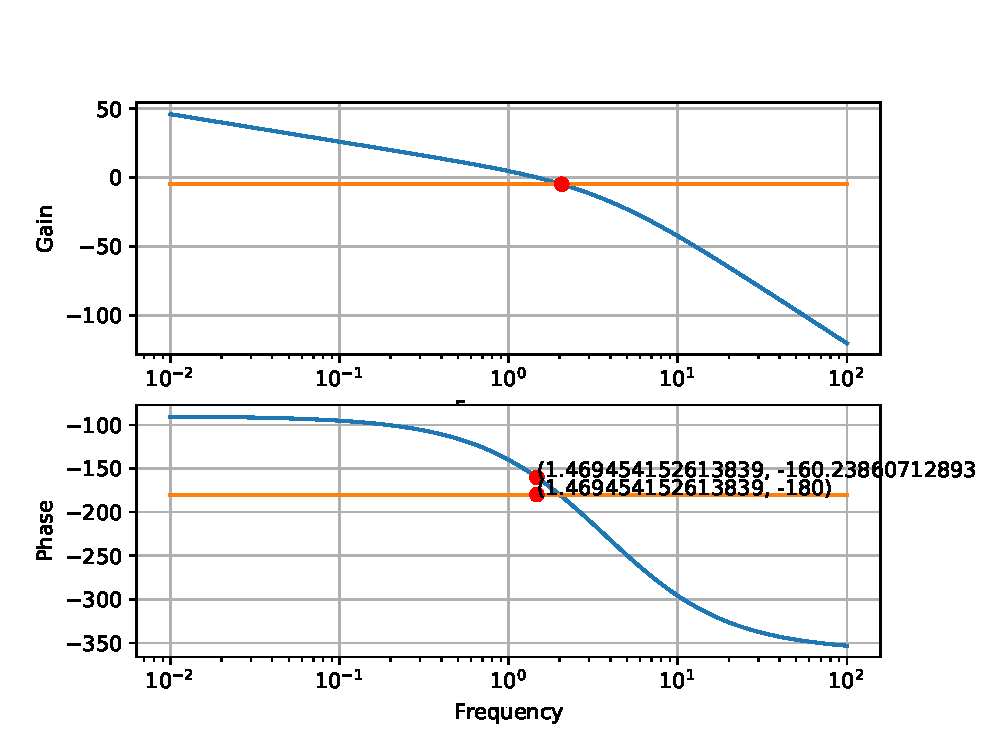
\includegraphics[width=\columnwidth]{./figs/ee18btech11036_1.eps}
  \caption{}
  \label{fig:ee18btech11036_1}
\end{figure}

Therefor amount of phase to be added: 30-19.76=10.24





%\item 
The circuit of lead compensator is given by
\begin{figure}[!ht]
    \centering
	\resizebox{\columnwidth}{!}{%\begin{figure}
\tikzstyle{block} = [draw, fill=blue!20, rectangle, 
    minimum height=1cm, minimum width=1cm]
\tikzstyle{sum} = [draw, fill=blue!20, circle, node distance=1cm]
\tikzstyle{input} = [coordinate]
\tikzstyle{output} = [coordinate]
\tikzstyle{pinstyle} = [pin edge={to-,thin,black}]

% The block diagram code is probably more verbose than necessary
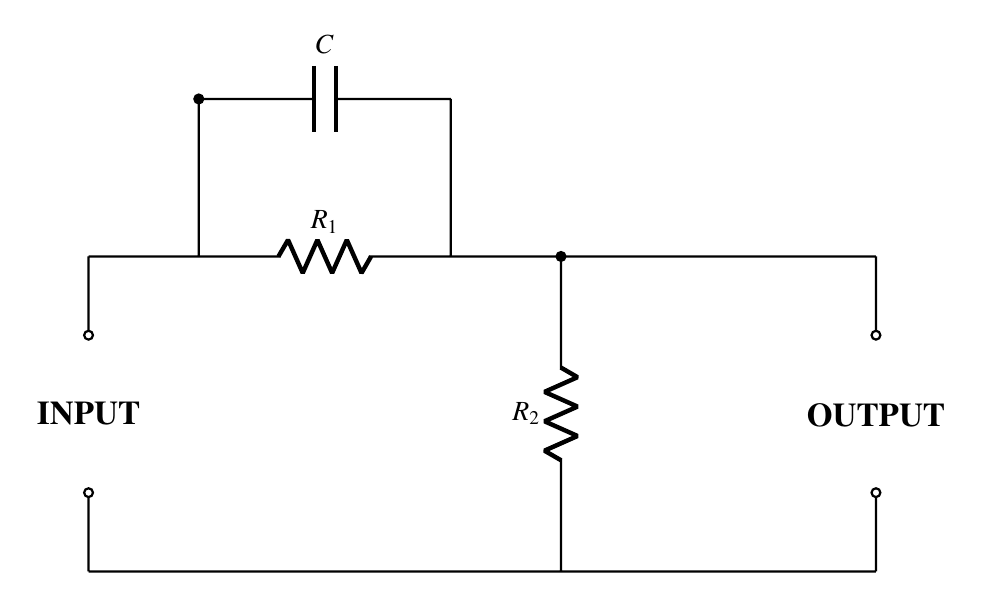
\begin{tikzpicture}[scale=2]
    \draw[color=black, thick]
    (0,0) to (5,0){} 
    (0,2) to [short,-o] (0,1.5){}
    (0,0) to [short,-o] (0,0.5){}
    (0,1) node[]{\large{\textbf{INPUT}}}
    (0,2) to [R,l=$R_1$,](3,2)
    (0.7,3) to [C, l=$C$, *-] (2.3,3)
    (0.7,2) to (0.7,3){}
    (2.3,2) to (2.3,3){}
    (3,0) to [R,l=$R_2$,-*] (3,2)
    (3,2) to (5,2){}
    (5,2) to [short,-o] (5,1.5){}
    (5,0) to [short,-o] (5,0.5){} node[above=7mm]{\large{\textbf{OUTPUT}}}
    ;
\end{tikzpicture}
%\end{figure}

}
\caption{}
\label{fig:ee18btech11036_ckt}
\end{figure}

Transfer function:
\begin{align}
C(s)=\beta\brak{\frac{1+j\tau\omega}{1+j\beta\tau\omega}}
\label{eq:ee18btech11036_compensator}
\end{align}

\begin{align}
\beta=\brak{\frac{R_2}{R_1+R_2}}\\
\tau =R_1C
\label{eq:ee18btech11036_values}
\end{align}
Find the values of $\beta$ and $\tau$\\
\solution The maximum phase lead compensated by a lead compensator is given by\\
\begin{align}
\phi={\sin}^{-1}\frac{1-\beta}{1+\beta}
\label{eq:ee18btech11036_beta}
\end{align}
at
\begin{align}
\omega =\frac{1}{\sqrt{\beta}\tau}
\label{eq:ee18btech11036_omega}
\end{align}

Now we know that from Gain crossover frequency
\begin{align}
\omega =1.469 rad/sec
\end{align}
and the phase margin to be added:
\begin{align}
\phi =10.24\degree
\end{align}
But to compensate for the added magnitude of lead compensator, a correction factor of $10\degree-20\degree$
is added.Hence
\begin{align}
\phi =30.24\degree
\implies \beta=0.33
\end{align}
From the bode plot $\omega$ is chosen at which gain of original system is
\begin{align}
-20\log\brak{1/\sqrt{\beta}}&=-4.81
\end{align}
\begin{figure}[!ht]
  \centering
  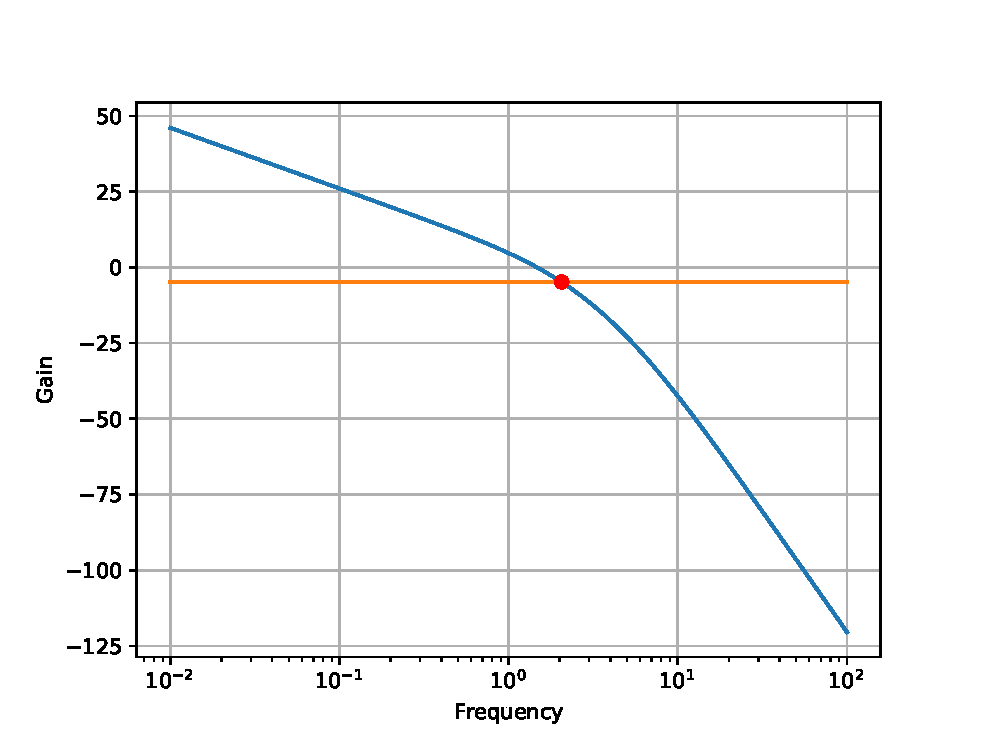
\includegraphics[width=\columnwidth]{./figs/ee18btech11036_3.eps}
  \caption{}
  \label{fig:ee18btech11036_3}
\end{figure}
Find the plot using the following code
\begin{lstlisting}
codes/ee18btech11036_4.py
\end{lstlisting}
From plot $\omega$=2.009 rad/sec\\
Solving equations \ref{eq:ee18btech11036_beta} and \ref{eq:ee18btech11036_omega}:
\begin{align}
\tau= 0.828\\
\beta=0.33\\
\label{eq:ee18btech11036_final}
\end{align}

New Transfer Function:
\begin{align}
G(s)=\frac{96\brak{1+ 0.828s}}{\brak{s}\brak{2+s}\brak{4+s}\brak{6+s}\brak{1+0.273s}}
\end{align}


\begin{figure}[!ht]
    \centering
	\resizebox{\columnwidth}{!}{%\begin{figure}
\tikzstyle{block} = [draw, fill=blue!20, rectangle, 
    minimum height=1cm, minimum width=1cm]
\tikzstyle{sum} = [draw, fill=blue!20, circle, node distance=1cm]
\tikzstyle{input} = [coordinate]
\tikzstyle{output} = [coordinate]
\tikzstyle{pinstyle} = [pin edge={to-,thin,black}]

% The block diagram code is probably more verbose than necessary
\begin{tikzpicture}[auto, node distance=2cm,>=latex']
    % We start by placing the blocks
    \node [input, name=input] {};
    \node [sum, right of=input] (sum) {};
    \node [block, right of=sum] (controller) {$ \beta(\frac{1+s\tau}{1+s\beta\tau})$};
    \node [block, right of=controller,
            node distance=3cm] (system) {$G(s)$};
    % We draw an edge between the controller and system block to 
    % calculate the coordinate u. We need it to place the measurement block. 
    \draw [->] (controller) -- node[name=u] {$U(s)$} (system);
    \node [output, right of=system] (output) {};
    \node [block, below of=u] (measurements) {1};

    % Once the nodes are placed, connecting them is easy. 
    \draw [draw,->] (input) -- node {$R(s)$} (sum);
    \draw [->] (sum) -- node {$E(s)$} (controller);
    \draw [->] (system) -- node [name=y] {$C(s)$}(output);
    \draw [->] (y) |- (measurements);
    \draw [->] (measurements) -| node[pos=0.99] {$-$} node [near end] {} (sum);
\end{tikzpicture}
%\end{figure}

}
\caption{}
\label{fig:ee18btech11036_fin}
\end{figure}


%\item
Verify your results from the following code:
\begin{lstlisting}
codes/ee18btech11036_2.py
\end{lstlisting}
\begin{itemize}
    \item The Phase margin: $29.269\degree$
    \item The Gain Crossover Frequency: 2.02 rad/sec
\end{itemize}
%
The Bode plot is as shown,
\begin{figure}[!ht]
  \centering
  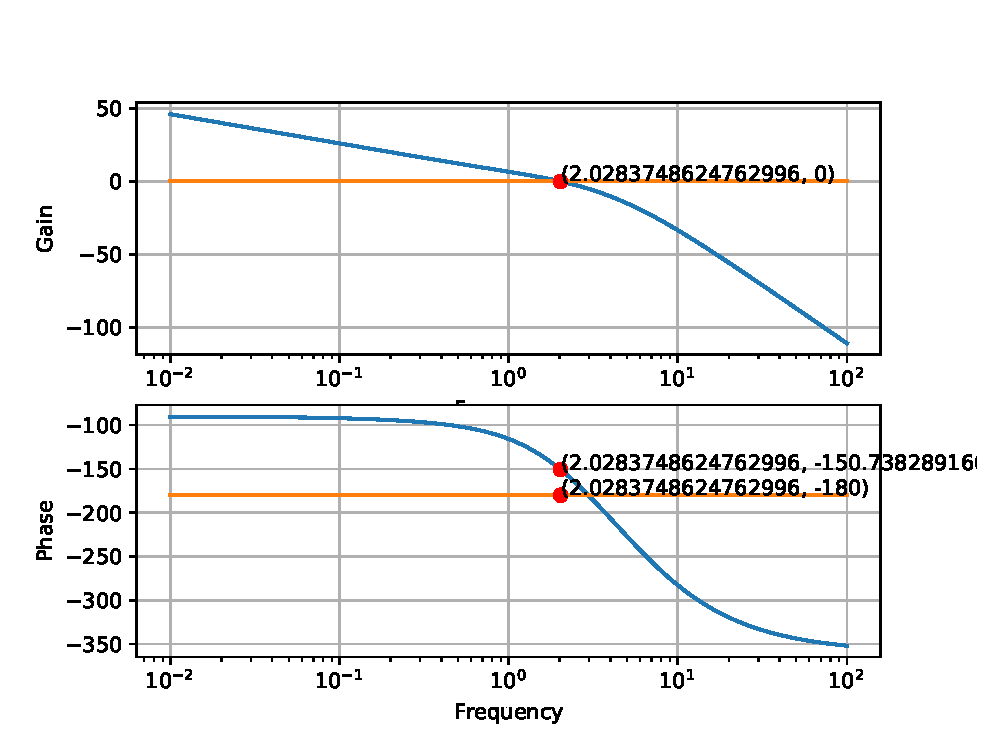
\includegraphics[width=\columnwidth]{./figs/ee18btech11036_2.eps}
  \caption{}
  \label{fig:ee18btech11036_2}
\end{figure}


%\end{enumerate}

\end{enumerate}
\subsection{}
\subsection{}
\subsection{Lead Compensator}
\begin{enumerate}[label=\thesubsection.\arabic*.,ref=\thesubsection.\theenumi]
\numberwithin{equation}{enumi}
%\begin{enumerate}[label=\thesection.\arabic*.,ref=\thesection.\theenumi]
%\numberwithin{equation}{enumi}
\item An aircraft roll control system can be represented by a block diagram shown in Fig. \ref{fig:es17btech11002_block} with G\brak{s} in feedback system, whose error  $K_v$ = 5. Determine K 
\begin{align}
G\brak{s} &= \frac{10K}{s\brak{s+1}\brak{s+5}}
\label{eq:es17btech11002_system}
\end{align}
%\item 
The block diagram is given by Fig.\ref{fig:es17btech11002_block}
\begin{figure}[!ht]
 \centering
     \resizebox{\columnwidth}{!}{
\tikzstyle{block} = [draw, fill=white!20, rectangle, 
    minimum height=3em, minimum width=4em]
\tikzstyle{sum} = [draw, fill=white!20, circle, node distance=1cm]
\tikzstyle{input} = [coordinate]
\tikzstyle{output} = [coordinate]
\tikzstyle{pinstyle} = [pin edge={to-,thin,black}]
\begin{tikzpicture}[auto, node distance=2cm,>=latex']
    % We start by placing the blocks
    \node [input, name=input] {};
    \node [sum, right of=input,node distance=2cm] (sum) {$\sum_{}^{}$};
    \node [block, right of=sum] (controller) {$C(s)$};
    \node [block, right of=controller,
            node distance=2.5cm] (system) {G(s)};
    % We draw an edge between the controller and system block to 
    % calculate the coordinate u. We need it to place the measurement block. 
    \draw [->] (controller) -- node[name=u] {} (system);
    \node [output, right of=system] (output) {};
    \coordinate [below of=u] (tmp);

    % Once the nodes are placed, connecting them is easy. 
    \draw [draw,->] (input) -- node  {$X(s) $} (sum);
    \draw [->] (sum) -- node {$ $} (controller);
    \draw [->] (system) -- node [name=y] {$Y(s) $}(output);
    \draw [->] (input) -- node{$ $} node[pos=0.93]{$+$} (sum);
    \draw [->] (y) |- (tmp) -| node[pos=0.99] {$-$} 
        node [near end] {$ $} (sum);
    
\end{tikzpicture}
}
    \caption{}
    \label{fig:es17btech11002_block}
\end{figure}
%\\

%\item \solution 
For unity feedback we have Velocity error constant $\brak{K_v}$
\begin{align}
K_v &= \lim_{s \to 0} s G\brak{s} 
\end{align}
\begin{align}
\lim_{s \to 0} \brak{\frac{10K}{\brak{s+1}\brak{s+5}} }& = 5 \\
\implies K = 2.5
\end{align}
It's Phase Margin  = 3.94\degree\\
and Gain Crossover Frequency = 2.03 rad/s
Refer Fig. \ref{fig:es17btech11002_1} for plot G\brak{s}.
\begin{lstlisting}
codes/es17btech11002_1_new.py
\end{lstlisting}
\begin{figure}[!h]
\centering
  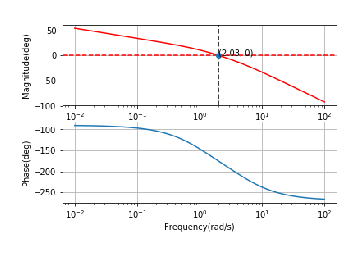
\includegraphics[width=\columnwidth]{./figs/es17btech11002_1_new.eps}
  \caption{}
  \label{fig:es17btech11002_1}
\end{figure}

%\item Design a Lag-Lead Compensator to yield a Phase margin\brak{PM} of 60\degree \\
%\solution 
Compensator required phase angle \brak{\phi_{m}} and  Phase Margin Frequency \brak{\omega_{pm}}, 
\begin{align}
    \phi_{m}= -\brak{180\degree+\theta}+PM+5 & =65\degree
    \\
    \omega_{pm}=1.25 rad/s.
\end{align}
Attenuation factor $\brak{\alpha\beta}$ is given by
\begin{align}
\alpha= 0.5
\\
\beta =  20
\end{align}
Lead and Lag Compensator Design Parameter is given in TABLE \ref{table:es17btech11002_1}
\begin{table}[!ht]
\centering
%%%%%%%%%%%%%%%%%%%%%%%%%%%%%%%%%%%%%%%%%%%%%%%%%%%%%%%%%%%%%%%%%%%%%%
%%                                                                  %%
%%  This is the header of a LaTeX2e file exported from Gnumeric.    %%
%%                                                                  %%
%%  This file can be compiled as it stands or included in another   %%
%%  LaTeX document. The table is based on the longtable package so  %%
%%  the longtable options (headers, footers...) can be set in the   %%
%%  preamble section below (see PRAMBLE).                           %%
%%                                                                  %%
%%  To include the file in another, the following two lines must be %%
%%  in the including file:                                          %%
%%        \def\inputGnumericTable{}                                 %%
%%  at the beginning of the file and:                               %%
%%        \input{name-of-this-file.tex}                             %%
%%  where the table is to be placed. Note also that the including   %%
%%  file must use the following packages for the table to be        %%
%%  rendered correctly:                                             %%
%%    \usepackage[latin1]{inputenc}                                 %%
%%    \usepackage{color}                                            %%
%%    \usepackage{array}                                            %%
%%    \usepackage{longtable}                                        %%
%%    \usepackage{calc}                                             %%
%%    \usepackage{multirow}                                         %%
%%    \usepackage{hhline}                                           %%
%%    \usepackage{ifthen}                                           %%
%%  optionally (for landscape tables embedded in another document): %%
%%    \usepackage{lscape}                                           %%
%%                                                                  %%
%%%%%%%%%%%%%%%%%%%%%%%%%%%%%%%%%%%%%%%%%%%%%%%%%%%%%%%%%%%%%%%%%%%%%%



%%  This section checks if we are begin input into another file or  %%
%%  the file will be compiled alone. First use a macro taken from   %%
%%  the TeXbook ex 7.7 (suggestion of Han-Wen Nienhuys).            %%
\def\ifundefined#1{\expandafter\ifx\csname#1\endcsname\relax}


%%  Check for the \def token for inputed files. If it is not        %%
%%  defined, the file will be processed as a standalone and the     %%
%%  preamble will be used.                                          %%
\ifundefined{inputGnumericTable}

%%  We must be able to close or not the document at the end.        %%
	\def\gnumericTableEnd{\end{document}}


%%%%%%%%%%%%%%%%%%%%%%%%%%%%%%%%%%%%%%%%%%%%%%%%%%%%%%%%%%%%%%%%%%%%%%
%%                                                                  %%
%%  This is the PREAMBLE. Change these values to get the right      %%
%%  paper size and other niceties. Uncomment the landscape option   %%
%%  to the documentclass defintion for standalone documents.        %%
%%                                                                  %%
%%%%%%%%%%%%%%%%%%%%%%%%%%%%%%%%%%%%%%%%%%%%%%%%%%%%%%%%%%%%%%%%%%%%%%

	\documentclass[12pt%
			  %,landscape%
                    ]{report}
       \usepackage[latin1]{inputenc}
	\usepackage{fullpage}
	\usepackage{color}
       \usepackage{array}
	\usepackage{longtable}
       \usepackage{calc}
       \usepackage{multirow}
       \usepackage{hhline}
       \usepackage{ifthen}

	\begin{document}


%%  End of the preamble for the standalone. The next section is for %%
%%  documents which are included into other LaTeX2e files.          %%
\else

%%  We are not a stand alone document. For a regular table, we will %%
%%  have no preamble and only define the closing to mean nothing.   %%
    \def\gnumericTableEnd{}

%%  If we want landscape mode in an embedded document, comment out  %%
%%  the line above and uncomment the two below. The table will      %%
%%  begin on a new page and run in landscape mode.                  %%
%       \def\gnumericTableEnd{\end{landscape}}
%       \begin{landscape}


%%  End of the else clause for this file being \input.              %%
\fi

%%%%%%%%%%%%%%%%%%%%%%%%%%%%%%%%%%%%%%%%%%%%%%%%%%%%%%%%%%%%%%%%%%%%%%
%%                                                                  %%
%%  The rest is the gnumeric table, except for the closing          %%
%%  statement. Changes below will alter the table's appearance.     %%
%%                                                                  %%
%%%%%%%%%%%%%%%%%%%%%%%%%%%%%%%%%%%%%%%%%%%%%%%%%%%%%%%%%%%%%%%%%%%%%%

\providecommand{\gnumericmathit}[1]{#1} 
%%  Uncomment the next line if you would like your numbers to be in %%
%%  italics if they are italizised in the gnumeric table.           %%
%\renewcommand{\gnumericmathit}[1]{\mathit{#1}}
\providecommand{\gnumericPB}[1]%
{\let\gnumericTemp=\\#1\let\\=\gnumericTemp\hspace{0pt}}
 \ifundefined{gnumericTableWidthDefined}
        \newlength{\gnumericTableWidth}
        \newlength{\gnumericTableWidthComplete}
        \newlength{\gnumericMultiRowLength}
        \global\def\gnumericTableWidthDefined{}
 \fi
%% The following setting protects this code from babel shorthands.  %%
 \ifthenelse{\isundefined{\languageshorthands}}{}{\languageshorthands{english}}
%%  The default table format retains the relative column widths of  %%
%%  gnumeric. They can easily be changed to c, r or l. In that case %%
%%  you may want to comment out the next line and uncomment the one %%
%%  thereafter                                                      %%
\providecommand\gnumbox{\makebox[0pt]}
%%\providecommand\gnumbox[1][]{\makebox}

%% to adjust positions in multirow situations                       %%
\setlength{\bigstrutjot}{\jot}
\setlength{\extrarowheight}{\doublerulesep}

%%  The \setlongtables command keeps column widths the same across  %%
%%  pages. Simply comment out next line for varying column widths.  %%
\setlongtables

\setlength\gnumericTableWidth{%
	40pt+%
	25pt+%
	35pt+%
	91pt+%
0pt}
\def\gumericNumCols{4}
\setlength\gnumericTableWidthComplete{\gnumericTableWidth+%
         \tabcolsep*\gumericNumCols*2+\arrayrulewidth*\gumericNumCols}
\ifthenelse{\lengthtest{\gnumericTableWidthComplete > \linewidth}}%
         {\def\gnumericScale{\ratio{\linewidth-%
                        \tabcolsep*\gumericNumCols*2-%
                        \arrayrulewidth*\gumericNumCols}%
{\gnumericTableWidth}}}%
{\def\gnumericScale{1}}

%%%%%%%%%%%%%%%%%%%%%%%%%%%%%%%%%%%%%%%%%%%%%%%%%%%%%%%%%%%%%%%%%%%%%%
%%                                                                  %%
%% The following are the widths of the various columns. We are      %%
%% defining them here because then they are easier to change.       %%
%% Depending on the cell formats we may use them more than once.    %%
%%                                                                  %%
%%%%%%%%%%%%%%%%%%%%%%%%%%%%%%%%%%%%%%%%%%%%%%%%%%%%%%%%%%%%%%%%%%%%%%

\ifthenelse{\isundefined{\gnumericColA}}{\newlength{\gnumericColA}}{}\settowidth{\gnumericColA}{\begin{tabular}{@{}p{65pt*\gnumericScale}@{}}x\end{tabular}}
\ifthenelse{\isundefined{\gnumericColB}}{\newlength{\gnumericColB}}{}\settowidth{\gnumericColB}{\begin{tabular}{@{}p{65pt*\gnumericScale}@{}}x\end{tabular}}
\ifthenelse{\isundefined{\gnumericColC}}{\newlength{\gnumericColC}}{}\settowidth{\gnumericColC}{\begin{tabular}{@{}p{65pt*\gnumericScale}@{}}x\end{tabular}}

\begin{tabular}[c]{%
	b{\gnumericColA}%
	b{\gnumericColB}%
	b{\gnumericColC}%
	}

%%%%%%%%%%%%%%%%%%%%%%%%%%%%%%%%%%%%%%%%%%%%%%%%%%%%%%%%%%%%%%%%%%%%%%
%%  The longtable options. (Caption, headers... see Goosens, p.124) %%
%	\caption{The Table Caption.}             \\	%
% \hline	% Across the top of the table.
%%  The rest of these options are table rows which are placed on    %%
%%  the first, last or every page. Use \multicolumn if you want.    %%

%%  Header for the first page.                                      %%
%	\multicolumn{4}{c}{The First Header} \\ \hline 
%	\multicolumn{1}{c}{colTag}	%Column 1
%	&\multicolumn{1}{c}{colTag}	%Column 2
%	&\multicolumn{1}{c}{colTag}	%Column 3
%	&\multicolumn{1}{c}{colTag}	\\ \hline %Last column
%	\endfirsthead

%%  The running header definition.                                  %%
%	\hline
%	\multicolumn{4}{l}{\ldots\small\slshape continued} \\ \hline
%	\multicolumn{1}{c}{colTag}	%Column 1
%	&\multicolumn{1}{c}{colTag}	%Column 2
%	&\multicolumn{1}{c}{colTag}	%Column 3
%	&\multicolumn{1}{c}{colTag}	\\ \hline %Last column
%	\endhead

%%  The running footer definition.                                  %%
%	\hline
%	\multicolumn{4}{r}{\small\slshape continued\ldots} \\
%	\endfoot

%%  The ending footer definition.                                   %%
%	\multicolumn{4}{c}{That's all folks} \\ \hline 
%	\endlastfoot
%%%%%%%%%%%%%%%%%%%%%%%%%%%%%%%%%%%%%%%%%%%%%%%%%%%%%%%%%%%%%%%%%%%%%%

\hhline{|-|-|-}
	 \multicolumn{1}{|p{\gnumericColA}|}%
	{\gnumericPB{\centering}\gnumbox{\textbf{Zeros/Poles}}}
	&\multicolumn{1}{p{\gnumericColB}|}%
	{\gnumericPB{\raggedright}\gnumbox[l]{\textbf{Parameter}}}
	&\multicolumn{1}{p{\gnumericColC}|}%
	{\gnumericPB{\raggedright}\gnumbox[l]{\textbf{Value}}}
\\
\hhline{|---|}
	 \multicolumn{1}{|p{\gnumericColA}|}%
	{$z_{lead}$}
	&\multicolumn{1}{p{\gnumericColB}|}%
	{$\omega_{pm}\sqrt{\alpha}$}
	&\multicolumn{1}{p{\gnumericColC}|}%
	{\gnumericPB{\centering}\gnumbox{0.279}}
\\
\hhline{|---|}
	 \multicolumn{1}{|p{\gnumericColA}|}%
	{$p_{lead}$}
	&\multicolumn{1}{p{\gnumericColB}|}%
	{$\frac{z_{lead}}{\alpha}$}
	&\multicolumn{1}{p{\gnumericColC}|}%
	{\gnumericPB{\centering}\gnumbox{5.590}}
\\
\hhline{|---|}
	 \multicolumn{1}{|p{\gnumericColA}|}%
	{$z_{lag}$}
	&\multicolumn{1}{p{\gnumericColB}|}%
	{$0.1\omega_{pm}$}
	&\multicolumn{1}{p{\gnumericColC}|}%
	{\gnumericPB{\centering}\gnumbox{0.125}}
\\
\hhline{|---|}
	 \multicolumn{1}{|p{\gnumericColA}|}%
	{$p_{lag}$}
	&\multicolumn{1}{p{\gnumericColB}|}%
	{$\frac{z_{lag}}{\beta}$}
	&\multicolumn{1}{p{\gnumericColC}|}%
	{\gnumericPB{\centering}\gnumbox{0.00625}}
\\
\hhline{|-|-|-|}


%---------------------------------------------------------------------------
\end{tabular}

\ifthenelse{\isundefined{\languageshorthands}}{}{\languageshorthands{\languagename}}
\gnumericTableEnd

\caption{Zeroes and Poles}
\label{table:es17btech11002_1}
\end{table}
And Compensator obtained has transfer function
\begin{align}
    G_{c}\brak{s}= \frac{\brak{s+0.279}\brak{s+0.125}}{\brak{s+5.590}\brak{s+0.00625}}
\end{align}

%\item Plot the graph after adding Lead-Lag compensator.
%\\
%\solution 
Refer Fig\ref{fig:es17btech11002_2} for plot $G\brak{s}G_{c}\brak{s}$.
\begin{lstlisting}
codes/es17btech11002_2_new.py
\end{lstlisting}
\begin{figure}[!h]
\centering
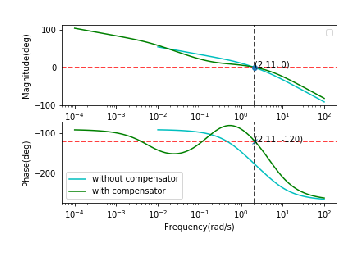
\includegraphics[width=\columnwidth]{./figs/es17btech11002_2_new.eps}
\caption{}
\label{fig:es17btech11002_2}
\end{figure}

\textbf{NOTE :} The idea of using a lead-lag network is to provide the attenuation of a phase-lag network and the lead-phase angle of a phase-lead
network. This points should be noted while designing a controller, and parameters to be changed accordingly to get exact results.
%\end{enumerate}     

\end{enumerate}
\subsection{}
\subsection{}
\subsection{}

\section{PID Controller Design}
\subsection{Introduction}
%%%%%%%%%%%%%%%%%%%%%%%%%%%%%%%%%%%%%%%%%%%%%%%%%%%%%%%%%%%%%%%%%%%%%%
%%                                                                  %%
%%  This is the header of a LaTeX2e file exported from Gnumeric.    %%
%%                                                                  %%
%%  This file can be compiled as it stands or included in another   %%
%%  LaTeX document. The table is based on the longtable package so  %%
%%  the longtable options (headers, footers...) can be set in the   %%
%%  preamble section below (see PRAMBLE).                           %%
%%                                                                  %%
%%  To include the file in another, the following two lines must be %%
%%  in the including file:                                          %%
%%        \def\inputGnumericTable{}                                 %%
%%  at the beginning of the file and:                               %%
%%        \input{name-of-this-file.tex}                             %%
%%  where the table is to be placed. Note also that the including   %%
%%  file must use the following packages for the table to be        %%
%%  rendered correctly:                                             %%
%%    \usepackage[latin1]{inputenc}                                 %%
%%    \usepackage{color}                                            %%
%%    \usepackage{array}                                            %%
%%    \usepackage{longtable}                                        %%
%%    \usepackage{calc}                                             %%
%%    \usepackage{multirow}                                         %%
%%    \usepackage{hhline}                                           %%
%%    \usepackage{ifthen}                                           %%
%%  optionally (for landscape tables embedded in another document): %%
%%    \usepackage{lscape}                                           %%
%%                                                                  %%
%%%%%%%%%%%%%%%%%%%%%%%%%%%%%%%%%%%%%%%%%%%%%%%%%%%%%%%%%%%%%%%%%%%%%%



%%  This section checks if we are begin input into another file or  %%
%%  the file will be compiled alone. First use a macro taken from   %%
%%  the TeXbook ex 7.7 (suggestion of Han-Wen Nienhuys).            %%
\def\ifundefined#1{\expandafter\ifx\csname#1\endcsname\relax}


%%  Check for the \def token for inputed files. If it is not        %%
%%  defined, the file will be processed as a standalone and the     %%
%%  preamble will be used.                                          %%
\ifundefined{inputGnumericTable}

%%  We must be able to close or not the document at the end.        %%
	\def\gnumericTableEnd{\end{document}}


%%%%%%%%%%%%%%%%%%%%%%%%%%%%%%%%%%%%%%%%%%%%%%%%%%%%%%%%%%%%%%%%%%%%%%
%%                                                                  %%
%%  This is the PREAMBLE. Change these values to get the right      %%
%%  paper size and other niceties.                                  %%
%%                                                                  %%
%%%%%%%%%%%%%%%%%%%%%%%%%%%%%%%%%%%%%%%%%%%%%%%%%%%%%%%%%%%%%%%%%%%%%%

	\documentclass[12pt%
			  %,landscape%
                    ]{report}
       \usepackage[latin1]{inputenc}
       \usepackage{fullpage}
       \usepackage{color}
       \usepackage{array}
       \usepackage{longtable}
       \usepackage{calc}
       \usepackage{multirow}
       \usepackage{hhline}
       \usepackage{ifthen}

	\begin{document}


%%  End of the preamble for the standalone. The next section is for %%
%%  documents which are included into other LaTeX2e files.          %%
\else

%%  We are not a stand alone document. For a regular table, we will %%
%%  have no preamble and only define the closing to mean nothing.   %%
    \def\gnumericTableEnd{}

%%  If we want landscape mode in an embedded document, comment out  %%
%%  the line above and uncomment the two below. The table will      %%
%%  begin on a new page and run in landscape mode.                  %%
%       \def\gnumericTableEnd{\end{landscape}}
%       \begin{landscape}


%%  End of the else clause for this file being \input.              %%
\fi

%%%%%%%%%%%%%%%%%%%%%%%%%%%%%%%%%%%%%%%%%%%%%%%%%%%%%%%%%%%%%%%%%%%%%%
%%                                                                  %%
%%  The rest is the gnumeric table, except for the closing          %%
%%  statement. Changes below will alter the table's appearance.     %%
%%                                                                  %%
%%%%%%%%%%%%%%%%%%%%%%%%%%%%%%%%%%%%%%%%%%%%%%%%%%%%%%%%%%%%%%%%%%%%%%

\providecommand{\gnumericmathit}[1]{#1} 
%%  Uncomment the next line if you would like your numbers to be in %%
%%  italics if they are italizised in the gnumeric table.           %%
%\renewcommand{\gnumericmathit}[1]{\mathit{#1}}
\providecommand{\gnumericPB}[1]%
{\let\gnumericTemp=\\#1\let\\=\gnumericTemp\hspace{0pt}}
 \ifundefined{gnumericTableWidthDefined}
        \newlength{\gnumericTableWidth}
        \newlength{\gnumericTableWidthComplete}
        \newlength{\gnumericMultiRowLength}
        \global\def\gnumericTableWidthDefined{}
 \fi
%% The following setting protects this code from babel shorthands.  %%
 \ifthenelse{\isundefined{\languageshorthands}}{}{\languageshorthands{english}}
%%  The default table format retains the relative column widths of  %%
%%  gnumeric. They can easily be changed to c, r or l. In that case %%
%%  you may want to comment out the next line and uncomment the one %%
%%  thereafter                                                      %%
\providecommand\gnumbox{\makebox[0pt]}
%%\providecommand\gnumbox[1][]{\makebox}

%% to adjust positions in multirow situations                       %%
\setlength{\bigstrutjot}{\jot}
\setlength{\extrarowheight}{\doublerulesep}

%%  The \setlongtables command keeps column widths the same across  %%
%%  pages. Simply comment out next line for varying column widths.  %%
\setlongtables

\setlength\gnumericTableWidth{%
	53pt+%
	93pt+%
0pt}
\def\gumericNumCols{2}
\setlength\gnumericTableWidthComplete{\gnumericTableWidth+%
         \tabcolsep*\gumericNumCols*2+\arrayrulewidth*\gumericNumCols}
\ifthenelse{\lengthtest{\gnumericTableWidthComplete > \linewidth}}%
         {\def\gnumericScale{\ratio{\linewidth-%
                        \tabcolsep*\gumericNumCols*2-%
                        \arrayrulewidth*\gumericNumCols}%
{\gnumericTableWidth}}}%
{\def\gnumericScale{1}}

%%%%%%%%%%%%%%%%%%%%%%%%%%%%%%%%%%%%%%%%%%%%%%%%%%%%%%%%%%%%%%%%%%%%%%
%%                                                                  %%
%% The following are the widths of the various columns. We are      %%
%% defining them here because then they are easier to change.       %%
%% Depending on the cell formats we may use them more than once.    %%
%%                                                                  %%
%%%%%%%%%%%%%%%%%%%%%%%%%%%%%%%%%%%%%%%%%%%%%%%%%%%%%%%%%%%%%%%%%%%%%%

\ifthenelse{\isundefined{\gnumericColA}}{\newlength{\gnumericColA}}{}\settowidth{\gnumericColA}{\begin{tabular}{@{}p{53pt*\gnumericScale}@{}}x\end{tabular}}
\ifthenelse{\isundefined{\gnumericColB}}{\newlength{\gnumericColB}}{}\settowidth{\gnumericColB}{\begin{tabular}{@{}p{93pt*\gnumericScale}@{}}x\end{tabular}}

\begin{tabular}[c]{%
	b{\gnumericColA}%
	b{\gnumericColB}%
	}

%%%%%%%%%%%%%%%%%%%%%%%%%%%%%%%%%%%%%%%%%%%%%%%%%%%%%%%%%%%%%%%%%%%%%%
%%  The longtable options. (Caption, headers... see Goosens, p.124) %%
%	\caption{The Table Caption.}             \\	%
% \hline	% Across the top of the table.
%%  The rest of these options are table rows which are placed on    %%
%%  the first, last or every page. Use \multicolumn if you want.    %%

%%  Header for the first page.                                      %%
%	\multicolumn{2}{c}{The First Header} \\ \hline 
%	\multicolumn{1}{c}{colTag}	%Column 1
%	&\multicolumn{1}{c}{colTag}	\\ \hline %Last column
%	\endfirsthead

%%  The running header definition.                                  %%
%	\hline
%	\multicolumn{2}{l}{\ldots\small\slshape continued} \\ \hline
%	\multicolumn{1}{c}{colTag}	%Column 1
%	&\multicolumn{1}{c}{colTag}	\\ \hline %Last column
%	\endhead

%%  The running footer definition.                                  %%
%	\hline
%	\multicolumn{2}{r}{\small\slshape continued\ldots} \\
%	\endfoot

%%  The ending footer definition.                                   %%
%	\multicolumn{2}{c}{That's all folks} \\ \hline 
%	\endlastfoot
%%%%%%%%%%%%%%%%%%%%%%%%%%%%%%%%%%%%%%%%%%%%%%%%%%%%%%%%%%%%%%%%%%%%%%

\hhline{|-|-}
	 \multicolumn{1}{|p{\gnumericColA}|}%
	{\gnumericPB{\centering}\gnumbox{\textbf{Controller}}}
	&\multicolumn{1}{p{\gnumericColB}|}%
	{\gnumericPB{\centering}\gnumbox{\textbf{Gain}}}
\\
\hhline{|--|}
	 \multicolumn{1}{|p{\gnumericColA}|}%
	{\gnumericPB{\centering}\gnumbox{PID}}
	&\multicolumn{1}{p{\gnumericColB}|}%
	{$    K_{p}\brak{1 + T_{d}s + \frac{1}{T_{i}s}}$}
\\
\hhline{|--|}
	 \multicolumn{1}{|p{\gnumericColA}|}%
	{\gnumericPB{\centering}\gnumbox{PD}}
	&\multicolumn{1}{p{\gnumericColB}|}%
	{$    K_{p}(1 + T_{d}s)$}
\\
\hhline{|--|}
	 \multicolumn{1}{|p{\gnumericColA}|}%
	{\gnumericPB{\centering}\gnumbox{PI}}
	&\multicolumn{1}{p{\gnumericColB}|}%
	{$    K_{p}\brak{1 +  \frac{1}{T_{i}s}}$}
\\
\hhline{|-|-|}
\end{tabular}

\ifthenelse{\isundefined{\languageshorthands}}{}{\languageshorthands{\languagename}}
\gnumericTableEnd


%
%


\end{document}


